\documentclass[12pt,twoside]{article}
\usepackage[T1]{fontenc}
\usepackage{multirow}
\usepackage[english]{babel}
% Language setting
% Replace `english' with e.g. `spanish' to change the document language

% Set page size and margins
% Replace `letterpaper' with `a4paper' for UK/EU standard size
%\usepackage[a4paper,top=2cm,bottom=2cm,left=3cm,right=3cm,marginparwidth=1.75cm]{geometry}
\usepackage[letterpaper,top=2cm,bottom=2cm,left=3cm,right=3cm,marginparwidth=1.75cm]{geometry}
\linespread{1.25}
%\usepackage[a4paper]{geometry}
% Useful packages
\usepackage{fancyhdr}
\usepackage{url}
\usepackage{pifont}
\usepackage{amsmath}
\usepackage{amssymb}
\usepackage{graphicx}
\usepackage[colorlinks=true, allcolors=blue]{hyperref}
%\usepackage{hyperref}
\usepackage[version=4]{mhchem}
\usepackage{titlesec}
\usepackage{caption}
%\usepackage{subfigure}
\usepackage{subcaption}
\usepackage{enumitem}
\usepackage{multirow} 
\usepackage{authblk}
\usepackage{tabularx}
\usepackage{sidecap}
\usepackage{makecell}
\newcommand{\RM}[1]{\MakeUppercase{\romannumeral #1}}
\usepackage[all]{hypcap}
\usepackage{fancybox}
\usepackage{pdfpages}
\usepackage{titlesec}
\usepackage[nottoc]{tocbibind}
\usepackage[capitalise]{cleveref}
\usepackage{floatrow}
\usepackage[thinc]{esdiff}
\usepackage[toc,page]{appendix}
\newfloatcommand{capbtabbox}{table}[\tiny][\FBwidth]

\title{Introduction}
\author{Tobias}

\begin{document}
%\maketitle
  \begin{titlepage}
\thispagestyle{empty}

\begin{center}
  
\includegraphics[width=0.25\textwidth]{Figures/TUMLogo_oZ_Outline_blau_CMYK-eps-converted-to.pdf}
  
  \vspace{1em}
  \Large TUM School of Natural Sciences\\
  \vspace{1em}
  \large Technische Universit\"at M\"unchen\\
   \vspace{0.5em}
  %\large FACHBEREICH: DENSE AND STRANGE HADRONIC MATTER (E62)\\
  \vspace{0.5em}
  
\end{center}

{% Create the command for including the title page in the document
  \centering % Center all text
  \vspace*{\baselineskip} % White space at the top of the page
  
  % Thick+thin horizontal line
%   \rule{\textwidth}{1.6pt}\vspace*{-\baselineskip}\vspace*{2pt} 
%   \rule{\textwidth}{0.4pt}\\[\baselineskip]
  
  % Title
%   {\Huge \textbf{\MakeUppercase{Pion Beam detector}} 
%     \\[0.3\baselineskip] %
%     \textbf{\MakeUppercase{for}} \\[0.3\baselineskip]
%     \textbf{\MakeUppercase{the HADES Experiment}} \\[0.5\baselineskip] }
	{\Large Nuclear Structure Investigations of Light Nuclei \\[0.3\baselineskip] with the R$^3$B Experiment   \\[0.3\baselineskip]
	}

  % Thin horizontal line
%   \rule{\textwidth}{0.4pt}\vspace*{-\baselineskip}\vspace{3.2pt}
%   \rule{\textwidth}{1.6pt}\\[\baselineskip] % Thick horizontal line
  
  %\scshape % Small caps
  
  % SubTitle
  {Tobias Jenegger}
  
  \vspace*{2\baselineskip} % Whitespace between location/year and editors

	Vollst\"andiger Abdruck der von der TUM School of Natural Sciences der Technischen
	Universit\"at M\"unchen zur Erlangung des akademischen Grades eines

	\vspace*{2ex}
	Doktors der Naturwissenschaften (Dr. rer. nat.)
	\vspace*{2ex}

	genehmigten Dissertation.

  \vspace*{\fill}

% 	\begin{tabularx}{1.0\textwidth}{XX}
% 	Vorsitzende:	&	Prof. Dr. Nora Brambilla \\
% 	Prüfer der Dissertation:	&	1. Univ.-Prof. Dr. Laura Fabbietti \\
% 							&	2. Prof. Dr. Lothar Oberauer \\
% 	\end{tabularx}
% 
% 
% 	\vspace*{\fill}
% 
% 	Die Dissertation wurde am xx.04.2016 bei der Technischen Universität München
% 	eingereicht und durch die Fakultät für Physik am xx.04.2015 angenommen.

  	\begin{tabularx}{1.0\textwidth}{XX}
	Vorsitz:	&	TBA \\
	Pr\"ufer*innen der Dissertation:	&	1. TBA \\
							        &	2. TBA \\
							
	\end{tabularx}


	\vspace*{\fill}

	Die Dissertation wurde am DATUM-HIER bei der Technischen Universit\"at M\"unchen
	eingereicht und durch die TUM School of Natural Sciences am DATUM-HIER angenommen.

  \vspace*{\fill}

  \null
  \vfill

%   {\scshape 2016} \\[0.3\baselineskip] % Year published }
}
\end{titlepage}

\newpage\null\thispagestyle{empty}\newpage

\thispagestyle{empty}
\newgeometry{%
  top=1in,%
  bottom=1in,%
  left=1.0in,%
  right=1.0in,%
  hmarginratio=2:1%
}
\begin{center}
  
\includegraphics[width=0.3\textwidth]{Figures/TUMLogo_oZ_Outline_blau_CMYK-eps-converted-to.pdf}
  
  \vspace{3mm}
  \huge TUM School of Natural Sciences
  \vspace{3mm}  
  
\end{center}

{% Create the command for including the title page in the document
  \centering % Center all text
  \vspace*{\baselineskip} % White space at the top of the page
  
  % Thick+thin horizontal line
  \rule{\textwidth}{1.6pt}\vspace*{-\baselineskip}\vspace*{2pt} 
  \rule{\textwidth}{0.4pt}\\[\baselineskip]
  
  % Title
%   {\Huge \textbf{\MakeUppercase{Pion Beam detector}} 
%     \\[0.3\baselineskip] %
%     \textbf{\MakeUppercase{for}} \\[0.3\baselineskip]
%     \textbf{\MakeUppercase{the HADES Experiment}} \\[0.5\baselineskip] }

	{\Large Nuclear Structure Investigations of Light Nuclei \\[0.3\baselineskip] with the R$^3$B Experiment   \\[0.3\baselineskip]
	}

  % Thin horizontal line
  \rule{\textwidth}{0.4pt}\vspace*{-\baselineskip}\vspace{3.2pt}
  \rule{\textwidth}{2pt}\\[\baselineskip] % Thick horizontal line
  
  %\scshape % Small caps
  
  % SubTitle
  {\Huge Tobias Jenegger }
  
  \vspace*{2\baselineskip} % Whitespace between location/year and editors
  
  % Edited by \\[\baselineskip]
  % 
  % \begin{minipage}{0.8\textwidth}
  % % \Large
  % \makeatletter
  % \@author
  % \makeatother
  % \end{minipage}
  
%   \vspace{15pt} % Whitespace between editor names and publisher logo
  \vspace*{\fill}
  
  % {\Huge {\textbf{For internal use only}} }
  
  % \begin{figure*}[!h]
  %  \hspace{0.15\textwidth}%
  %  \includegraphics[width=0.5\textwidth,angle=15]{figures/ForInternalUseOnly}
  % \end{figure*}
  
  
%   \vspace{20pt} % Whitespace between editor names and publisher logo
  \vspace*{\fill}
  
  
  
  
\includegraphics[width=0.15\textwidth]{Figures/PH_CMYK-eps-converted-to.pdf}
  \\[0.3\baselineskip] % Publisher logo
  
  \null
  \vfill
  
  \vspace{1em}
  \large Techinsche Universit\"at M\"unchen\\
   \vspace{0.5em}
  \large Fachbereich: Dense and Strange Hadronic Matter (E62)\\
  \vspace{0.5em}
  
  {\scshape 2025} \\[0.3\baselineskip] % Year published }
  
}

\newpage\null\thispagestyle{empty}\newpage

\newgeometry{left=18mm,right=18mm, top=16mm, bottom=16mm}
\thispagestyle{empty}
\section*{Abstract}
The nucleosynthesis of heavy elements (A > 56) beyond iron, primarily via the rapid neutron-capture process (r-process), represents one of the most fascinating and complex phenomena in nuclear astrophysics. This process, which is responsible for the majority of heavy element production in the universe, provides a critical interface between astrophysics and nuclear physics, offering a unique "laboratory" to study nuclear reactions and properties far from stability. Neutron stars (NS), with their extreme densities and exotic compositions, are of exceptional interest in this context. These astrophysical objects serve as a natural laboratory to explore nuclear structure under extreme conditions, such as those described by the equation of state (EoS). Understanding the EoS, which governs the macroscopic properties of neutron stars, remains a formidable challenge. While astrophysical observations provide macroscopic constraints on NS models, nuclear experiments in terrestrial laboratories play a vital role in constraining the microscopic nuclear physics parameters embedded within these models.
Moreover, neutron star mergers (NSMs), which are stellar collisions involving NSs, are recognized as the primary astrophysical sites for the r-process. These events generate conditions favorable for the production of neutron-rich nuclei, driving the synthesis of heavy elements. A comprehensive understanding of the r-process requires detailed knowledge of nuclear structure and reaction dynamics in regimes far from nuclear stability. However, experimental constraints on critical observables, such as fission yields and fission barriers, are limited due to the challenges associated with producing and studying these neutron-rich nuclei in laboratory settings.
This doctoral thesis, titled "Nuclear Structure Investigations of Light Nuclei with the R3B Experiment", addresses these challenges by presenting the analysis of two key reaction channels using carbon isotopes. These investigations were conducted with the R3B (Reactions with Relativistic Radioactive Beams) setup during the commissioning experiment S444 as part of the FAIR Phase-0 campaign at GSI. Specifically, this work focuses on:
\begin{enumerate}
\item Charge-changing and total interaction cross sections: The study of 12C+12C collisions via the transmission method. These measurements provide critical insights into the nuclear structure and reaction mechanisms of light nuclei, which serve as essential benchmarks for understanding nuclear matter in astrophysical environments.
\item Quasi-free scattering (QFS) reactions: The investigation of the 12C(p,2p)11B reaction as a tool to probe nuclear structure. This approach demonstrates its potential for studying the dynamics of the r-process through fission in QFS experiments, offering an innovative method to address experimental limitations in current r-process studies.
\end{enumerate}
The results of these analyses contribute to our understanding of the structure of light nuclei and provide critical experimental constraints relevant to nuclear astrophysics. By advancing our knowledge of fundamental nuclear properties and reaction dynamics, this work bridges the gap between laboratory-based nuclear physics and astrophysical processes, shedding light on the origin of heavy elements in the universe.


\newpage\null\thispagestyle{empty}\newpage

%\include{Zusammenfassung}

\newpage\null\thispagestyle{empty}\newpage


\restoregeometry
\pagenumbering{roman}
\setcounter{page}{1}
\tableofcontents
\newpage
\pagenumbering{arabic}
\pagestyle{headings}
%\pagestyle{fancy}
%\fancyfoot{}
\section{Introduction}
The elemental abundances observed throughout the universe are a fingerprint of the formation and evolution of astrophysical objects. Understanding the origin and distribution of these elements requires a robust theoretical framework based on nuclear structure models. The synthesis of elements -- from the lightest nuclei formed during Big Bang nucleosynthesis to the heaviest transuranic elements produced in explosive astrophysical environments -- depends critically on the properties of atomic nuclei.\newline
The foundation for modern nuclear structure theory was laid by the atomic shell model, first introduced by Niels Bohr in 1913. This model, while initially developed for electrons in atoms, inspired the formulation of the nuclear shell model by Maria Goeppert Mayer and J. Hans D. Jensen in 1949. Their key innovation was the inclusion of a significant spin-orbit interaction term in the nuclear mean-field potential. Unlike the atomic case -- where spin-orbit coupling appears as a relatively small fine-structure correction -- in the nuclear shell model, the spin-orbit interaction is of comparable magnitude to the primary energy level gaps and carries an inverted sign. This results in the $j = l + 1/2$ states lying energetically below the $j = l - 1/2$  states.\newline
This critical adjustment enabled the nuclear shell model to accurately reproduce the so-called "magic numbers" (2, 8, 20, 28, 50, 82, and 126), which correspond to closed shells of protons or neutrons associated with exceptional nuclear stability. Notable examples include isotopes such as those of thin (Z = 50) and  lead ( Z = 82), where large energy gaps between filled and unfilled shells lead to enhanced binding energies and structural rigidity.\newline
While the shell model has proven highly successful in describing nuclei close to stability, recent experiments have shown, that the magic shells can be substantially modified in case of exotic species, like $^{32}$Mg \cite{wimmer2010discovery} or $^{28}$O \cite{kanungo2009one}. In case of more heavy regions, experimental data remain scarce, and the shell model must be extended or augmented to account for collective phenomena and configuration mixing. These nuclei play a central role in rapid neutron-capture processes (r-process), which are responsible for the formation of approximately half of the heavy elements beyond iron. In particular, the fate of the r-process path -- its termination via fission and the possible emergence of a predicted "island of stability" in the superheavy region -- depends critically on the structural properties of such exotic nuclei.\newline
This chapter introduces the scientific objectives and research program of the R$^3$B experiment. In particular, we highlight the role of nuclear structure studies in constraining the nuclear equation of state (EOS), especially for highly asymmetric nuclear matter. Nuclear scattering reactions at R$^3$B offer an effective probe of these systems, and their theoretical treatment -- along with a general overview of reaction mechanisms -- will be presented in chapter \ref{sec:reac_model}.

\subsection{R$^3$B Experiment - "The Universe in the Lab"}
\subsubsection{Scientific Objectives and Research Program of the R3B Experiment at FAIR}
The R3B experiment (Reactions with Relativistic Radioactive Beams) is a key component of the nuclear astrophysics program at the Facility for Antiproton and Ion Research (FAIR) in Darmstadt and major experiment of the NUSTAR (\textbf{N}uclear \textbf{ST}ructure, \textbf{A}strophysics and \textbf{R}eactions) collaboration~\cite{krucken2005nustar}.\newline
As part of the broader research initiative \textit{"The Universe in the Lab"}, R3B aims to provide a comprehensive understanding of the fundamental nuclear processes that govern the formation of elements in the universe. It seeks to replicate, under controlled laboratory conditions, the extreme environments found in stellar explosions and neutron-star mergers -- astrophysical sites in which rapid nuclear reactions are responsible for the synthesis of the heavy elements~\cite{thielemann2017neutron}.\newline
The central scientific objective of R3B is the investigation of the structure and reaction dynamics of exotic, short-lived nuclei far from the valley of stability, particularly those involved in the rapid neutron-capture process (r-process) and other astrophysical nucleosynthesis pathways~\cite{horowitz2019r}. This includes the determination of key nuclear properties such as masses, lifetimes, decay modes, and reaction cross sections, as well as branching ratios and transition probabilities under conditions similar to those of astrophysical environments.\newline
To address these goals, R3B employs high-intensity, relativistic radioactive ion beams in conjunction with a versatile and high-resolution detectors capable of performing kinematically complete measurements of both incoming and outgoing reaction products. The experimental program covers a wide variety of reaction mechanisms, including fragmentation, Coulomb excitation, knockout, and charge-exchange reactions in inverse kinematics.\newline
As part of this thesis, one focus is placed on the quasi-free scattering reaction mechanism as a tool to study nuclear properties. A detailed discussion of the underlying reaction mechanism is provided in section~\ref{sec:qfs_theo}, while the corresponding data analysis based on the S444 experiment is presented in section~\ref{sec_analysis_qfs}.\newline
The R3B setup is specifically optimized for operation at beam energies of several hundred~MeV per nucleon. It provides precise tracking and unambiguous particle identification, with excellent resolution in time, energy, and position~\cite{heil2022new}. These capabilities are essential for disentangling complex reaction channels and for extracting high-precision nuclear data that serve as critical input to astrophysical models of nucleosynthesis.\newline
Directly related to the scientific objectives at R3B is the exploration of the equation of state (EoS) of asymmetric nuclear matter under extreme conditions. The EoS describes how nuclear matter behaves as a function of parameters such as density, temperature, and isospin asymmetry, and it plays a pivotal role in understanding a wide range of astrophysical phenomena, including the structure and evolution of neutron stars, core-collapse supernovae, and neutron star mergers.\newline

\subsubsection{Study of the EoS at R3B}

While various models agree at saturation density $n_0 \approx 0.16 fm^{-3}$  (natural packing density of nucleons inside a nucleus) at high baryon number density, as it is the case in neutron stars there are significant differences between the models. Fig X shows the EoS description for different models and their divergences by plotting the binding energy and the symmetry energy -- which will be introduced in the next paragraph -- versus the baryon number density. 
Huge efforts are made to constrain the EoS for highly asymmetric or pure neutron matter. \newline
In modeling the nuclear equation of state, it is common to perform a Taylor expansion of the energy per nucleon with respect to the isospin asymmetry parameter $\delta = \frac{n_n -n_p}{n_n + n_p}$ where $n_n$ and $n_p$ denote the neutron and proton number densities, respectively, at a fixed baryon density $n_B = n_n +n_p$. In this approach, the energy per nucleon is written as:
\begin{equation}\label{eq:eos}
E(n_B,\delta)=E(n_B,0)+S(n_B)\delta^2+\mathcal{O}(\delta^4)
\end{equation}
The second term on the left side of equation~\ref{eq:eos}  is called the asymmetry term. With:
\begin{equation}
S(n_B) = \frac{1}{2} \left. \frac{\partial^2 E(n, \delta)}{\partial \delta^2} \right|_{\delta = 0}
\end{equation}

This approach allows one to isolate the contribution of the symmetry energy $S(n_B)$  which governs the leading-order dependence on isospin asymmetry.\newline
To further understand how the symmetry energy evolves with density -- particularly in environments such as neutron stars -- $S(n_B) $is itself often expanded around the nuclear saturation density $n_0$ in a separate Taylor series involving the slope $L$ and curvature $K_{sym}$ parameters:
\begin{equation}
S(n_B) = S_0 + L \left( \frac{n_B - n_0}{3n_0} \right) + \frac{1}{2} K_{\text{sym}} \left( \frac{n_B - n_0}{3n_0} \right)^2 + \mathcal{O}\left(\left( \frac{n_B - n_0}{3n_0}\right)^4 \right)
\end{equation}
$S_0$ is constrained around 30-40 MeV which is compatible to the theoretical predictions. Both $L$ and $K$ are poorly constrained and according experimental data is limited. While the term with the curvature parameter $K$ enters quadratically, its contribution is small near to saturation density.\newline
Whereas the slope parameter L is the dominating factor. Constraining L, which quantifies the "stiffness" of the symmetry energy -- how much the energy cost of isospin asymmetry increases as nuclear matter becomes denser -- is of high interest and would lead to a better understanding of nuclear matter and its interaction, especially when considering extreme astrophysical object such as NS.\newline
Several physical approaches are currently being tested and refined in experimental nuclear physics to constrain L, amongst others in heavy ion collisions (for detailled informations see e.g. ~\cite{tsang2011constraints,tsang2024constraining,wang2020study,jhang2021symmetry} and via astrophysical observations (e.g. neutron star radii and mass measurements~\cite{bogdanov2021constraining,nattila2017neutron,radice2019multimessenger} and tidal deformability~\cite{hu2020effects,raithel2019measurement}).\\
For interest of the R3B experiment are the access points to constrain the slope parameter L by probing nuclear structure observables. There are two main approaches in this field:\\
\quad \textbf{Electric dipole polarizability $\alpha_D$}: As first pointed out by Reinhard and Nazarewicz~\cite{reinhard2010information} there is a strong correlation between the diplole polarizability $\alpha_D$ and the slope parameter L of the symmetry energy. First measurements of $\alpha_D$ have been performed at RCNP in Osaka -- for stable nuclei -- and at GSI for the neutron-rich short-lived nucleus $^{68}$Ni. The dipole polarizability $\alpha_D$ is experimentally accessible via the  Coulomb-excitation cross section $\sigma_C$ as shown in the work~\cite{horvat2021evolution} where a clear linear correlation between the polarizability $\alpha_D$ and the Coulomb-excitation cross section $\sigma_C$ is found.

%\begin{itemize}
%\item Heavy-Ion Collisions (HICs):
%	Observables such as isospin diffusion, neutron/proton yield ratios, and collective flows in intermediate-energy HICs are sensitive to the EoS.
%\item Electric Dipole Polarizability (α_D):
%	The dipole response of a nucleus to an external electric field reflects the symmetry energy.
%Measured via inelastic proton or alpha scattering and correlated with L through energy density functionals.
%\item Neuron Skin Thickness Measurements:
%\begin{itemize}
%\item PREX(Pb Radius Experiment): used parity-violating electron scattering on 208Pb to probe Δrnp​.
%Future experiments CREX (on 48Ca) aim to improve constraints.
%\item Neutron removal cross sections: 
%\end{itemize}
%\end{itemize}

%from ML: In particular, the density dependence of the symmetry energy, a key component of the nuclear EoS, remains poorly constrained at supra-saturation densities. The symmetry energy governs how the energy of nuclear matter changes as the neutron-to-proton ratio varies and has direct consequences for the composition and stability of neutron stars.




Central formula is the equation of states (EOS). We want to study it within a wide range. 
\begin{itemize}
\item in astrophysics NS are herefore of special interest. Measuring their mass and radius -> this relation depends on the EOS. 
\item since NS are highly asymmetric matter (neutrons only) they are a good playground to test the different models. Since they are all consistent at rho0 (real world) they diverge for higher matter asymmetry. 
\item plot of some models
\item formula of tailor expansion of Equation of state
\item at FAIR we want to study  nuclear matter under extreme conditions,highly asymmetric matter. 
\item constraining the symmetry energy
\item this can be done via neutron removal cross section, cite T. Aumann, Bertulani etc.
\item show picture of sensitiveness of this method, shortly mention that L was previously constrained in PREX experiments(give some literature for further readings)
\item the predicted models rely on the input from reaction mechanisms -> 12C+12C good to probe the underlying reaction mechanisms-> one part of the thesis
\end{itemize}
Moreover to study the single particle states of nucleons inside nucleus, especially when going toward exotic nuclei-> quasi free scattering experiments.-> refer to the theory of those scattering experiments
This was the first time we had our CALIFA CALORIMETER in its final frame. 
Refer to the application section. \newline
To point out is the pilot experiment we had in 2021 to study fission via qfs. This could have a large impact in the understanding of the dynamics of fission far off the line of stability. \newline
Explain the fission via qfs a little bit more in detail here.\newline
This could explain maybe better the element abundances we have and if there is any island of stability at Z > 126.


\section{Nuclear Scattering Reactions in the Glauber Framework}\label{sec:reac_model}
Explain path to go:
\begin{itemize}
\item short intro why we use scrattering reactions: to study structure of nuclei (mostly via e. scattering as they only interact via electromagn. force) and refer to chapter. Introduce problems qe account body problem etc
\item starting from elastic scattering at low energies going to medium to high energies
\item explain glauber: eikonal wave approximations, optical limit which leads to optical potential model, description via nucleon nucleon interaction
\end{itemize}
\subsection{Elastic scattering at low energies}
\begin{itemize}
\item Rutherford scattering,poiniering works (alpha particle on gold atoms),description in classical mechanics
\item Rutherford scattering only valid if coulomb potential
\item at low energies below pion production only elastic cross section
\item introduce here the Scattering problem in quantum mechanics (see Schindler, p. 23)
\item from classical physics we go to quantum mechanics and use partial wave decomposition with theta being the scattering angle
\item include in this picture coulomb and nuclear interaction (as done in Kuk, page 120)
\end{itemize}
\subsection{Nuclear Density distribution studies via elastic scattering}
\begin{itemize}
\item Rutherford, Mott and Rosenbluth
\item  show something about form Factors
\item  are charge radii and nuclear radii measured?
\item note approximation for $^{12}C$ that neutron radius same as proton radius
\end{itemize}
\subsection{Glauber Model for nuclear scattering at high energies}
\begin{itemize}
\item explain model assumption
\item eikonal wave approximation: high incoming momentum,low scattering angle
\item Show picture of scattering
\item optical limit: - Nucleons at high energy → undeflected due to large momentum (linear trajectory)
		   -Nucleus large compared to nucleon-nucleon  force
		   -Motion of nucleons independent of nucleus
		   -overall cross-section described in terms of nucleon-nucleon cross section
\item Description in the Probability Approach (also here I use all the eiconal and optical limit approximation)
\item Description in the Eikonal optical-limit approximation
\item Comparison of both descriptions methods  for total interaction cross section,should end up with same. Advantage of PA is that you can calculate the cross section for a defined number of removed projectile nucleons (Schindler, p. 49)
\end{itemize}
\subsubsection{Extensions to the Glauber model}
\begin{itemize}
\item things which cannot be neglected and influence the cross section
\item in medium modifications (see Lukas thesis)
\item Coulomb interaction
\item Pauli blocking
\end{itemize}
\subsection{Cross sections for $^{12}C + ^{12}C$}
\begin{itemize}
\item Total reaction cross section
\item charge changing cross section;maybe I have to include lise++ calculations
\item isotope corrections- neutron removal; maybe I have to include lise++ calculations
\end{itemize}

\subsection{Quasi-Free Scattering (QFS) Reactions}\label{sec:qfs_theo}
Quasi-free scattering (QFS) reactions, as a subset of direct reactions, are processes where a projectile nucleon interacts with a target nucleon via the strong nuclear force in a single and fast localized event at large momentum transfer which allows for a highly localized vertex. The relative kinetic energies of the participants, typically in the order of  $E_{kin}\gtrsim$ 100 AMeV, are high\footnote{Which is needed for the single nucleon-nucleon interaction.The \textit{de Broglie wavelength} of a 100 MeV proton corresponds to $\lambda \approx 2.79fm$ which is in the order of the proton diameter ($\approx 1.6 fm$)}.\newline
In QFS experiments conducted in direct kinematics, a proton serves as the projectile, colliding with a nucleon or a cluster within the target nucleus. Conversely, in inverse kinematics, the nucleus of interest becomes the projectile, while a proton or proton-like particle is used as the target. Despite these differing setups, both approaches are fundamentally equivalent, differing only due to a Lorentz transformation of the reference frame.\newline
As the name implies, QFS reactions are conceptually similar to free nucleon-nucleon scattering, with the primary approximation being that the influence of the residual nucleus is neglected to first order. This approximation simplifies the theoretical description of the process, allowing to treat the interaction as a two-body problem within a (only weakly interfering) nuclear environment.\newline
The first experiments confirming the existence of quasi-free scattering processes were conducted at the University of California, Berkeley, in 1952 by O. Chamberlain and Emilio Segr\`e\cite{chamberlain1952proton}. In their study, lithium nuclei were bombarded with 350 MeV protons, and coincident proton pairs were observed with an opening angle of approximately 90$^{\circ}$. That same year, J.B. Cladis, W.N. Hess, and B.J. Moyer published results on the scattering of 340 MeV protons on deuterium and carbon targets\cite{cladis1952nucleon}, further substantiating the phenomenon.\newline
In 1957, Tyr\'en, Maris, and Hillman designed an experiment aimed at fully characterizing proton-proton collisions within the quasi-free scattering framework\cite{MARIS19581}. Their results validated the assumption of a direct and clean interaction between the projectile and the target nucleon, free from significant distortions caused by the surrounding nucleus. Furthermore, these experiments demonstrated that QFS reactions could serve as a powerful tool for probing nuclear structure and testing predictions of the shell model. Specifically, they enabled the study of key nuclear parameters such as spin-orbit splitting and energy differences between nuclear shells probing the shell evolution. \newline
In QFS reactions, these parameters can be extracted by analyzing the reaction products, which include the two correlated outgoing protons, the residual nucleus, and any gamma rays emitted during de-excitation of the residual nucleus. The detailed measurements of these observables provide critical insights into the underlying nuclear structure and dynamics.\newline
The experimental discoveries and theoretical insights from these early studies strongly pushed the advancements in the theoretical modeling of QFS reactions. These models have since become essential tools for understanding nucleon-nucleon interactions within the nuclear medium and for further investigations of nuclear structure and reaction mechanisms.\newline
\subsubsection{Kinematics of QFS Reactions}\label{sec:kin_qfs}
A simplified picture, which however explains the essential kinematics of the QFS reaction, can be found in figure \ref{fig:sketch_qfs}: we have an incoming proton knocking out a nuclear constituent (proton/neutron) in a quasi-free nucleon-nucleon collision ending with a final state having the scattered proton, the scattered  off nuclear constituent and the rest nucleus (A-1), which could be either in the ground-state or an excited state. In this picture index \textit{0} is assigned to the incoming proton, \textit{1} to the knocked out nucleon, \textit{2} to the outgoing projectile proton, \textit{A} to the initial nucleus and  \textit{A-1} to the final nucleus accordingly.
\begin{figure}[htpb]
    \centering
    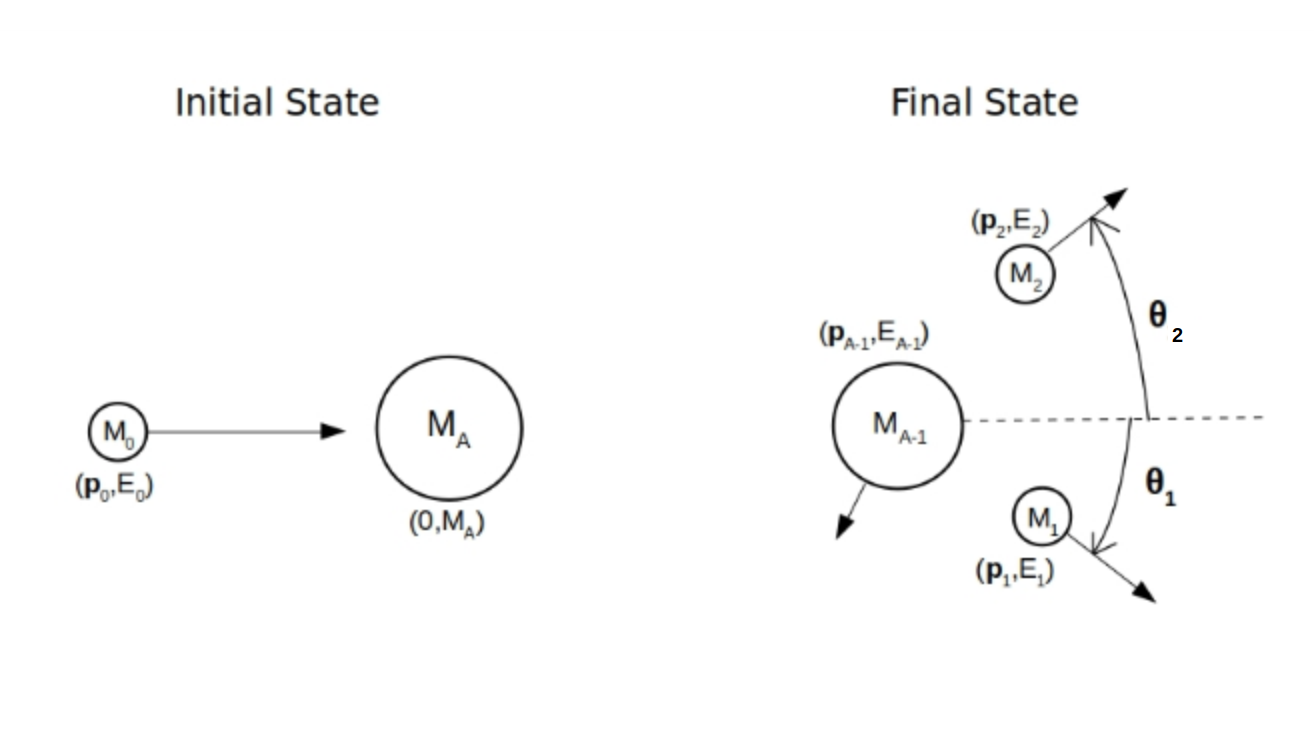
\includegraphics[width=\textwidth,height=8cm,keepaspectratio=true]{Figures/sketch_qfs.png}
    \caption{
   	Simplified picture of the QFS reaction process in direkt kinematics.  
    }
    \label{fig:sketch_qfs}
\end{figure}
From energy -momentum conservation the reaction can be expressed as:
\begin{equation}\label{eq:four_mom_cons_qfs}
P_A  +  P_0 = P_1 + P_2 +P_{A-1} 
\end{equation}
with $P_i$ the four momentum $(\mathbf{p_i},E_i)$.\newline
In direct kinematics as presented in figure \ref{fig:sketch_qfs} the separation energy  of the ejected nucleon for a certain final state of the nucleus \textit{A-1} is given by\footnote{In inverse kinematics the four-momentum vectors need to be boosted to the center of mass frame of the initial nucleus via Lorentz transformation.}:
\begin{equation}
S = T_0 -(T_1+T_2 +T_{A-1}); \; \text{with $T_i$ the kinetic energy of particle $i$} 
\label{eq:sep_e}
\end{equation}
In the idealized shell model the separation energy equals to the (negative) energy of the nucleus' single-particle state. For the case the proton knocks out the least bound nucleon (proton/neutron) the final nucleus is lying in the ground state with $E_{A-1} = M_{A-1}c^2  + T_{A-1}$.\newline
If a nucleon has been ejected from an inner shell resulting in a hole state, the final nucleus will be in an excited state:
\begin{equation}
E^{*}_{A-1} =  M_{A-1}c^2  +T_{A-1} + E_{exe}
\end{equation} 
The excitation energy $E_{exe}$ is reflected in the difference in the separation energy of the least bound nucleon and the ejected one. From the experimental point of view $E_{exe}$ is directly accessible via gamma detection from the transition of the final nucleus from the excited to the ground state.\newline
According to the picture of having a nucleon nucleon scattering process with no influence of the residual nucleus A-1 we can approximate the momenta of both constituents of the nucleus A with $\mathbf{p_A} \approx \mathbf{p_i} + \mathbf{p_{A-1}}$ where $\mathbf{p_i}$ is the initial nucleon momentum inside the initial nucleus A. Since the initial nucleus is at rest ($\mathbf{p_A} = 0$), the recoil momentum of the nucleus in final state $\mathbf{p_{A-1}}$ equals to $-\mathbf{p_i}$ the momentum of the initial nucleon pointing in opposite direction. \newline
In addition the four-momentum of the inner nucleon can be deduced from momentum measurement of the initial and final state free nucleons:
\begin{equation}\label{eq:miss_mom}
P_i \approx P_{miss} \equiv P_1 + P_2  - P_0
\end{equation}
where $P_{miss}$ is the so called "measured missing four-momentum of the reaction"\cite{patsyuk2021unperturbed}\footnote{$P_{miss}$ is only equal to $P_i$ for the unperturbed QFS (no ISI/FSI) case.}.
Thereupon, the separation energy measurement and the recoil momentum distribution fully describe the single paricle state in the various shell levels. 
In addition and as complementary method $\gamma$ rays can be measured in coincidence with the reaction and consequentely exclusive cross section and momentum distribution measurements of the single particle states are accessible as illustrated in figure blabla.\newline
Considering the removal of a single nucleon from an initial nucleus with A nucleons and initial spin \textit{I} $\Psi^A_i$ and final nucleus state  $\Psi^{A-1}_f$ with final spin $I_f$ an overlap function between intial and final state many-body wave function can be written as:
\begin{equation}
\langle \vec{r}, \Psi_f^{A^{-1}} | \Psi_i^A \rangle = \sum_j C_j^{if} \psi_j(\vec{r}), \quad with  |I - I_f| < j < |I + I_f|
\end{equation}
where $S_j^{if} = |C_j^{if}|^2$ is the commonly named spectroscopic factor, see ref \cite{hansen2003direct} sec.2.1. $S_j^{if}$ is summed over all final single particle states m (from $-j$ to $j$). It is unity for nucleon removal from a pure single particle state and equals (2j+1) when the nucleon was removed from a filled j-subshell.
The spectroscopic factor is linked to the exclusive experimental cross section measurement of a single particle state and the theoretical predicted one, as in ref \cite{hansen2003direct}:
\begin{equation}
\sigma_{th}^{if} = \sum_j S_j^{if}\,\sigma_{sp}(nlj)
\end{equation}
where $\sigma_{sp}$ are the theoretical cross sections for the normalized wave functions $\Psi_j$ of the final state nucleus A-1 with the appropriate quantum numbers.\newline
From this considerations the spectroscopic factor can be used to probe the theoretical shell predictions. In past this was already done with direct QFS-reactions $(e,e'p)$. Results for the spectroscopic factor with data obtained at the NIKHEF facility is shown in figure \ref{fig:spec_fac}. The substantial reduction of the spectroscopic factor with respect to the independent particle model (IPM) or mean field of $\approx 35\%$ indicates a substantial depletion of the single-hole states and inferring from this a refined model prediction has to be applied\footnote{The mean field potential does not consider spin-spin interaction $V_{ss}$, non central tensor-potential $V_T$ or spin-orbit interaction $V_{LS}$.}.\newline
\begin{figure}[h!]
    \centering
    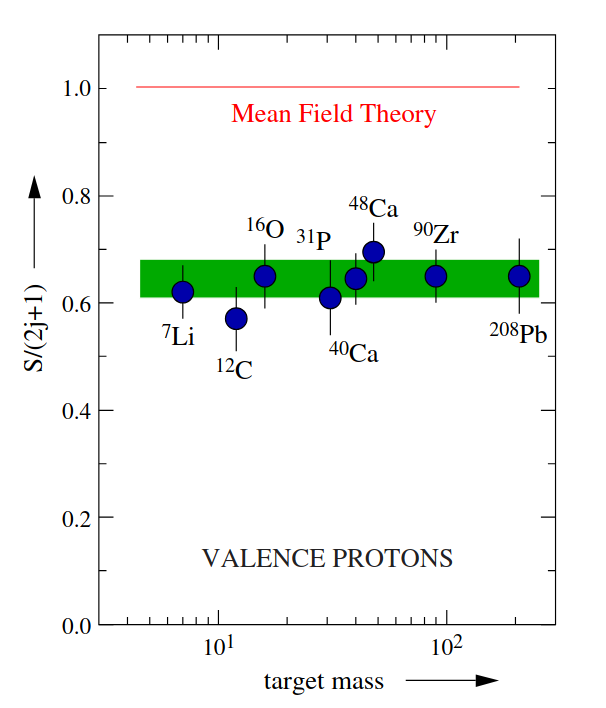
\includegraphics[width=\textwidth,height=8cm,keepaspectratio=true]{Figures/spec_factor.png}
    \caption{Normalized spectroscopic factors from the $(e,e'p)$ reaction as a function of target mass taken from \cite{DICKHOFF2004377}. As input for the theoretical cross sections the prediction from mean field models were used. }
    \label{fig:spec_fac}
\end{figure}
While QFS-reaction with electrons $(e,e'p)$ in direct kinematics is a valuable method to make precise measurements for stable (target) nuclei it is not suitable for the experimental analysis with exotic (neutron or proton rich) nuclei. Due to their unstability they have a short lifetime (e.g. $^{52}Ca$ with $\tau = 4.6s$) they can hardly serve as targets. Inducing the reaction in inverse kinematics - having electrons as targets and the exotic nuclei of interest as projectiles - is also not feasible since no free electons can be captured as target. The alternative approach is to use proton induced quasi-free scattering in inverse kinematics where the exotic beam inpinges on an extended proton target such as liquid hydrogen $H_2$  or a fixed proton rich target such as $CH_2$\footnote{Herefore a carbon target reference run is used to extract the QFS-reaction events from the $CH_2$ target run.}.\newline
Summarizing, the QFS-reaction technique in inverse kinematics with exotic nuclei as in-flight projectiles and a proton-like target opens new possibilities to probe theoretical model predictions of deformed nuclei far off stability which haven't been accessible before.\newline
For precise cross section measurements of the single particle states $\sigma_{sp}$ the kinematical characteristics of the QFS-reaction products have to be considered for correct identification of QFS-events and clear background substraction. The following descriptions are already implicitly embedded within the equation \ref{eq:four_mom_cons_qfs}.\newline
As starting point one compares the QFS-reaction of the two nucleons with the two dimensional non-central collision of free pointlike particles in nonrelativistic kinematics. Since both kinetic energy and momenta are conserved a  clear signature is expected: the opening angle of the scattered particles is exactly 90$^{\circ}$. 

However, at kinetic energies of 400 AMeV and more, relativistic effects affects the opening angle of the scattered particles\footnote{Relativistic considerations become relevant at velocities $ \beta \gtrapprox 0.1 c$. This corresponds to $\approx$ 4.5 MeV.}. 
TODO: Formula to calculate directly from beam energy the opening angle...

For the final description of the process it has to be considered that the projectile nucleon inside the nucleus has a non negligible momentum (see $P_i$ in equation \ref{eq:miss_mom})  and in addition the separation energy $S_{p/n}$ has to be expended to remove the scattered nucleon of the nuclear potential of the projectile nucleus.\newline
To account for the nucleon momentum the picture of the fermi gas model where protons and neutrons freely move inside the nucleus' potential is applied. In the ground state of the nucleus the nucleons can reach a momentum up to the Fermi momentum $p_F$. Except for the light nuclei, the Fermi momentum is almost independent of A and amounts to $\approx 250$ MeV/c \footnote{For light nuclei like $ ^{12}C$, $p_F \approx 230$ MeV/c can be assumed}. The mean quadratic momenta of the nucleons is related to the Fermi momentum by:
\begin{equation}
\langle \mathbf{p}^2 \rangle = \frac{3}{5}p^2_F \footnote{From the derivation of the mean kinetic energy of the nucleons $\langle E_{\text{kin}} \rangle = \frac{\int_0^{p_F} E_{\text{kin}} \, p^2 \, dp}{\int_0^{p_F} p^2 \, dp} = \frac{3}{5} \cdot \frac{p_F^2}{2M}$}
\end{equation}
The width of the momentum distribution of the nucleons is given in the Goldhaber model by:
\begin{equation}
\sigma^2 = \sigma_0^2 K(A-K)/(A-1), \, \text{with} \, \sigma_0 \approx 90 MeV/c
\end{equation}
where A is the mass number of the projectile nucleus and K the mass number of the fragment after scattering. For a detailed derivation and further readings see ref. \cite{goldhaber1974statistical} and \cite{FESHBACH1973300}.
In the impuse approximation, where we assume that the interaction between the projectile and target nucleons has approximately the same form as the interaction between two nucleons in free space, the inner momenta of the scattered nucleons smear out the angular correlations of the outgoing fragment - which has the same momentum as the knocked out nucleon in the cms system of the nucleus but points in opposite direction - as well as of the two nucleons involved in the scattering. As consequence the opening angle distribution of the two scattered nucleons gets broadened as well as the azimuthal angular correlation which for the assumption of zero nucleon momentum sharply peaked at $\Delta\varphi = 180^{\circ}$.\newline
In view of the added nucleon momentum the kinematics get expanded from a two dimensional scattering reaction to a three dimensional process where the reaction plane is determined by the plane spanned by the momentum vector of the projectile nucleus $\mathbf{p}_A$ and the scattered nucleon after the reaction \footnote{For (p,2p) reactions there is an ambigousity which of the scattered protons $\mathbf{p}_1$ or $\mathbf{p}_2$ origin from the projectile nucleus or the proton like target.}. With the momentum measurement of the two correlated outgoing nucleons and the momentum of the incoming projectile nucleus it is possible to retrieve the internal momentum of the knocked out nucleon perpendicular to the reaction plane via the formula derived in reference\cite{chulkov2005quasi}:
\begin{equation}\label{eq:chulkov}
Q_{\perp i} = sin(\theta_{1/2})\cdot sin(\varphi_{1/2} -\varphi_{2/1})\cdot\mathbf{p}_{2/1}
\end{equation}
In case of (p,2p) reactions it is impossible to track back the origin of each nucleon - from the projectile nucleus or the proton-like target. Iferrring from this there are two possible solutions for $Q_{\perp}$. The ambiguity can be resolved by incorporating the momentum of the fragment nucleus perpendicular to the reaction plane $Q_{\perp A-1}$. The fragment momentum vector should be of the same amout but point in opposite direction to $Q_{\perp i}$.
TODO: maybe insert here the plot of $Q_{\perp}$ if possible...


Up to this point the scattering process was described similar to the free elastic scattering in relativistic kinematics with the projectile nucleon having a non negligible momentum. However the projectile nucleon is an off-shell particle  bound inside the nucleus. 
\begin{equation}
\mu_i =  \sqrt{m_A^2 + m_{A-1}^2 + 2m_A\sqrt{m_{A-1}^2 + |\mathbf{p}_i|^2}}
\end{equation}
in the c.m.s. of the projectile nucleus, with
\begin{equation}
0 < \mu_i  < m_n
\end{equation}
where $m_n$ is the mass of the appropriate free nucleon.
To knock the bound nucleon out of the nucleus the separation energy has to be overcome which can be observed in the reduced opening angle of the two outgoing correlated nucleons.



%From experimental point of view-> important to identify the QFS events.
%In non rel. kinematics of free particles a really clean signature: two dim-colllision with coplanar nucleons = delta phi = 180 degr and an opening angle of 90 degr. \newline
%When going to rel. energies -> 80 degrees of opening angle(400 AMeV). Is there a function to calculate the opening angle? The opening angle is smeared because of relativistic effects + inner momentum of the nucleon. \newline
%Explain Goldhaber model to characterize the width of the inner momenta.\newline
%Plot the correlation plots of opening angle and delta phi.
%Then mentnion pronounced transversal correlation as in L.V. Chulkov -> insert image
%Moreover limited energy ranges are allowed where the forward nucleon has much higher energy compared to the larger scattered one -> insert image
%

\subsubsection{Cross Sections for QFS Reactions - Qualitative Considerations}
TO DO: see more in the standard work \cite{cladis1952nucleon}, \cite{MARIS19581}.
\subsubsection{Application Fields of QFS Reactions}
Over several decades of experimental and theoretical research, Quasi-Free Scattering (QFS) reactions have been firmly established as a powerful and direct tool for probing the microscopic structure of atomic nuclei. These reactions provide critical insights into nuclear correlations, single-particle properties, and the momentum distributions of nucleons within the nucleus.\newline
The versatility of QFS extends across various applications, including the study of short-range nucleon-nucleon interactions, exotic nuclear states, and the modification of nucleon properties in nuclear matter. Advances in experimental facilities and state-of-the-art detector systems, have significantly improved the precision and scope of QFS measurements. These developments have enabled in-depth investigations of nuclear dynamics, the structure of unstable isotopes, and fundamental aspects of quantum many-body systems, contributing to a deeper understanding of nuclear and subnuclear phenomena.\newline
This subsection will point out the most exciting and promising application fields of QFS reactions with focus on the applicability in the R$^3$B experimental setup. A detailed review can be found in ref \cite{panin2021quasi}.
\begin{description}
\item[Single-Particle Spectroscopic Strength]As already mentioned in section \ref{sec:kin_qfs} in many experiments a reduction in the spectroscopic strength of about 35\% with respect to the independent particle model (IPM) and shell model predictions was observed. In one-nucleon removal reactions - experiments with isotope beams impinging on a composite nuclear target - the extraction of the missing spectroscopic strength is challenging as the kinematical pattern is highly complex. In contrast, the QFS reactions mechanism in inverse kinematics retains a clear kinematical signature which makes it a valuable tool to study the quenching of the spectroscopic factor which originates from residual correlations between bound nucleons inside the nucleus. \newline
Several experiments were carried out at the GSI Facility to study the reduction factor of the spectroscopic strength  and its evolution over a broad range in isotopic chains, such as for oxygen shown in figure \ref{fig:red_factor}. With the commmissioning of the SIS100 and SuperFRS at GSI it will be achievable to study (p,2p) reactions with very short lived nuclei at reasonable intensities which will presumably draw even more attention to QFS reaction approach.  
\begin{figure}[htpb]
    \centering
    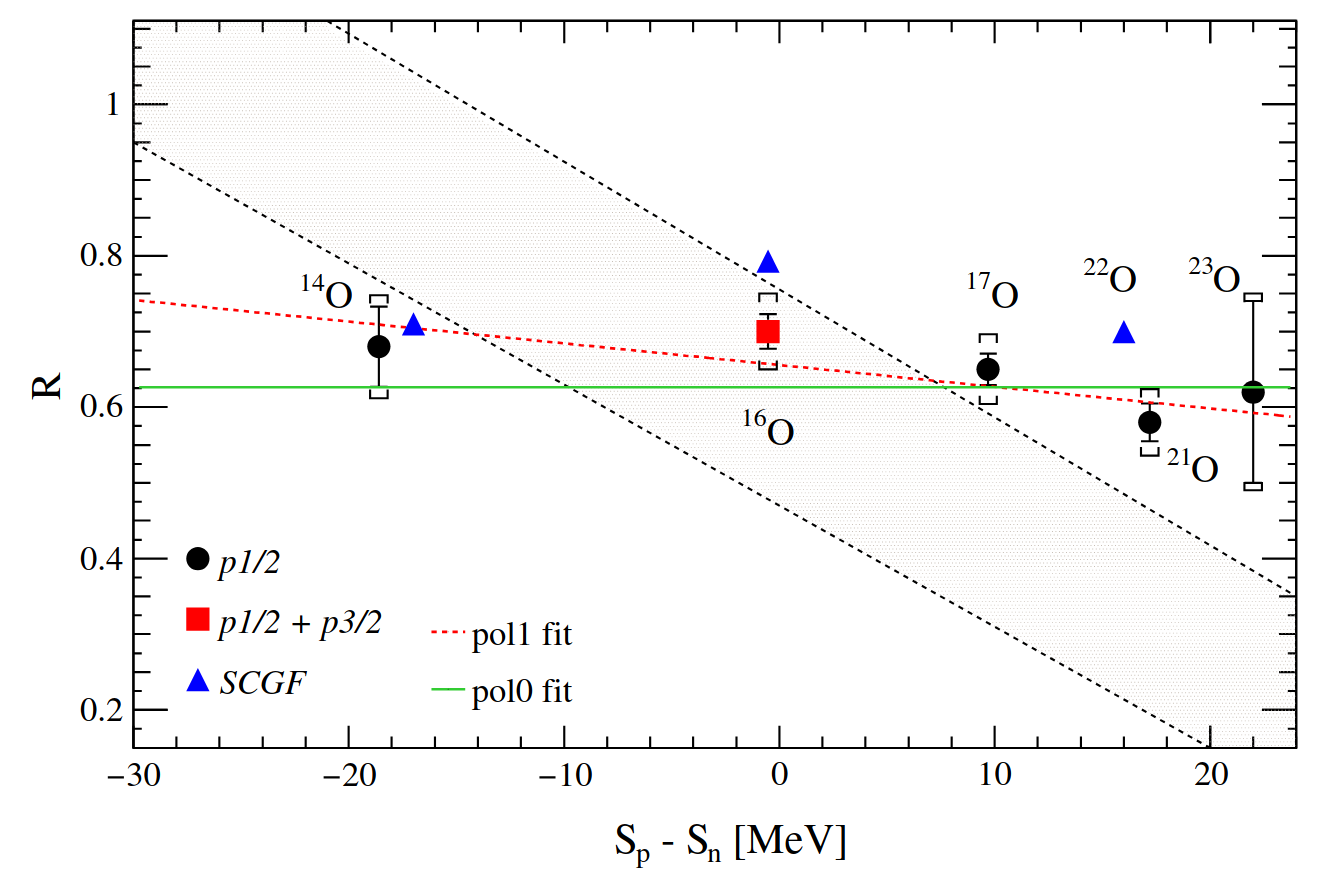
\includegraphics[width=\textwidth,height=8cm,keepaspectratio=true]{Figures/spec_red_factors.png}
    \caption{
   	Extracted reduction factors of the spectroscopic strength from (p,2p) measurements (circles and square) as a function of the difference between proton and neutron separation energy $S_p$/$S_n$. The blue triangles correspond to the predictions from self-consistent green functions (SCGF). The shaded area indicates the trend from an analysis of one-nucleon removal cross sections. From Ref. \cite{atar2018quasifree}.   
    }
    \label{fig:red_factor}
\end{figure}
\item[Gamma Spectroscopy]Alongside to the study of the single-particle spectroscopic strengths QFS reactions provide valuable information of the shell structure and deformation of the fragment (A-1) via gamma spectroscopy. While quasi-free scattering with nucleons in the outermost shell yield a fragment in the ground state, the scattering with nucleons in inner shells result in bound (or unbound) excited states of the (A-1) fragment. This excited fragment instantaneously transits to the ground state by the emission of a Doppler shifted $\gamma$ ray.\newline
A big advantage of the (p,2p) reaction experiments is ability to make precise vertex reconstruction by accurate measurement of the two outgoing correlated protons. This is of particular importance for extended targets and determines the emission point within the target, enabling an accurate calculation of the fragment\textquotesingle s velocity and therefore a precise Doppler correction.\newline
From gamma spectroscopy the excitation energy E(2+), often the first excited state in even-even nuclei, can be observed which is a fundamental observable of nuclear structure, providing key insights into the shell configuration and deformation of the nucleus\cite{panin2021quasi}. Expecially when going towards exotic neutron rich isotopes the study of the gamma emission lines can strongly contribute to the understanding of nuclear shell evolution.
\item[QFS to probe inner clustering and halo formation]Clusterization inside nuclei is a phenomenon widely observed in experimental astrophysics with large implications on processes such as the synthesis of carbon  inside stars via triple $\alpha$ clusterization \cite{hjorth2011carbon}, $\alpha$ - radioactivity, or the evolution of core collapse supernovae\cite{sumiyoshi2008appearance}, just to mention some. Its presence has also to be implemented in the state of the art equation of state calculations.\newline
Single-particle cluster states can be directly accessed via QFS (p,p$\alpha$) reactions. In the low energy regime of 100 AMeV the $^{12}\text{C}(p, p\alpha)^{8}\text{Be}$ reaction, see ref \cite{mabiala2009analyzing}, as benchmark study approved the reaction mechanism and up to a scaling factor the measured cross sections aligned exceptionally well to the free p–$\alpha$ scattering measurements.\newline
Moreover the QFS mechanism allows to acces light nuclei going towards the neutron drip line via (p,pn) reaction. These light nuclei are mostly weakly bound with an extended low density neutron-matter distribution forming a so-called \textit{nuclear-halo}.\newline
The most prominent candidate for such is $^{11}Li$, often called \textit{Borromean three-body system}\cite{johannsen199011li}, consisting of two neutrons interacting with a core ($^9Li$) via weak, short-range interactions. First evidence for the correlation  between the two neutron was strongly pushed by experimental studies at GSI, see \cite{simon1999direct}, and theoretical work by Bertulani et. al.\cite{bertulani2007geometry}.\newline
The latest experiment with the focus on the study of multi-neutron correlations in drip-line nuclei was carried out at R$^3$B in 2022 (experiment S509) probing broad isotopic chains of Li, Be, B, C and N via the QFS mechanism.
\item[Short Range Correlations(SRC)]Short range correlations refer to elementary nucleon-nucleon interactions within a nucleus and occur over very short distances, typically on the order of 1-2 femtometers.  These correlations are characterized by pairs of nucleons with high relative momentum ($> k_F$, Fermi momentum) and low total momentum. These NN-interactions are treated as good explanatory candidate for observed deviations from mean field approximation. Many phenomena, such as the above discussed reduction in the spectroscopic strength and the EMC effect\cite{xing2023electromagnetic}, the observation that  the cross section for deep inelastic scattering from an atomic nucleus is different from that of the same number of free protons and neutrons, are associated to the short range correlations inside the nucleus.\newline
From isotopic chain studies\cite{clas2018probing} it has been shown that there is an indication of SRC depenency on isospin, see figure \ref{fig:src_pairs}, where SRC are predominatly preferred by p-n pairs than by nn or pp pairs. This again can have significant impact for asymmetric nuclei and imply a stronger quenching of the spectroscopic strength for proton single particle states below the Fermi momentum for neutron rich matter.\newline  
Since pioneering experiments were made at JLab and Brookhaven via $(e,e'p)$ and $(e,e'n)$ reactions several  experimental campaigns were carried out at GSI with the R$^3$B setup probing the QFS reactions via the strong nuclear forceinstead of the Coulomb interaction. In 2022 the S509 experiment was performed to exploit for the first time the use of short-lived nuclei scattering off a proton probe in inverse kinematics at R$^3$B, followed by the S091 experiment in 2024 with the focus on probing NN-correlations in atomic nuclei via $(p,pd)$ QFS reactions\cite{paschalis2020nucleon}. 
\begin{figure}[htpb]
    \centering
    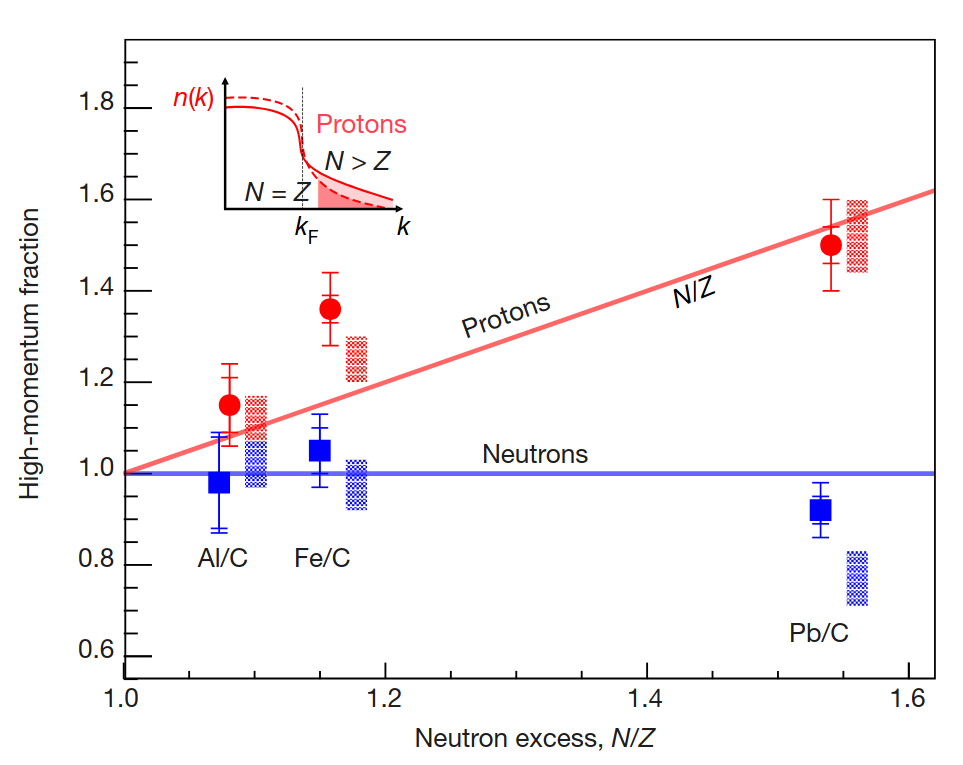
\includegraphics[width=\textwidth,height=8cm,keepaspectratio=true]{Figures/src_pn_excess.png}
    \caption{
   	Fraction of high-momentum neutrons and protons with respect to the N/Z ratio for several carbon isotopes. A clear trend towards high momentum proton distribution for neutron rich carbon isotopes (red line) is shown, while the high momentum neutron distribution stays constant wiht respect to the N/Z ratio (blue line). From reference \cite{clas2018probing}. 
    }
    \label{fig:src_pairs}
\end{figure}

\item[Fission via QFS]Fission induced via quasifree scattering (QFS) provides a powerful method to extract fission barriers on an event-by-event basis. The fundamental concept involves the knockout of a proton or neutron from an incoming exotic ion beam. By measuring the energy  and the angular distribution of the correlated emitted nucleons, it becomes possible to probe the excitation state of the daughter nucleus. In cases where deeply bound nucleons are knocked out, the resulting daughter nucleus either evaporates one or multiple neutrons or populates an excited state, which can be experimentally observed. The R$^3$B setup is particularly well-suited for such investigations, as it enables full kinematic reconstruction of the reaction products and hence to pin down the complete reaction mechanism. This approach allows for the detailed exploration of the potential-energy surface and the fission dynamics across a broad range of fissility and excitation energies, taking advantage of relativistic radioactive beams.\newline
A pilot experiment was conducted in 2021 at R$^3$B using a stable $^{238}$U beam incident on a liquid hydrogen target. The data collected from this experiment provide simultaneous information on several key fission observables, which can be used to constrain theoretical calculations. These calculations aim to describe both the static and dynamic properties of the fission process and enable comparisons with predictions from various theoretical frameworks, including phenomenological approaches, macroscopic-microscopic models, and fully microscopic statistical or time-dependent Hartree-Fock calculations.\newline
A critical aspect of this experimental setup is the simultaneous measurement of the two outgoing fission fragments. This is achieved using a dedicated ionization chamber (TWIM-MUSIC) and advanced tracking detectors. The success of this methodology has already been demonstrated by promising results, see \cite{garcia2023study},\cite{grana2023fission} and figure \ref{fig:qfs_fission}, highlighting the potential of this technique in advancing our understanding of nuclear fission dynamics.
\begin{figure}[htpb]
    \centering
    \begin{subfigure}[b]{0.3\textwidth}
    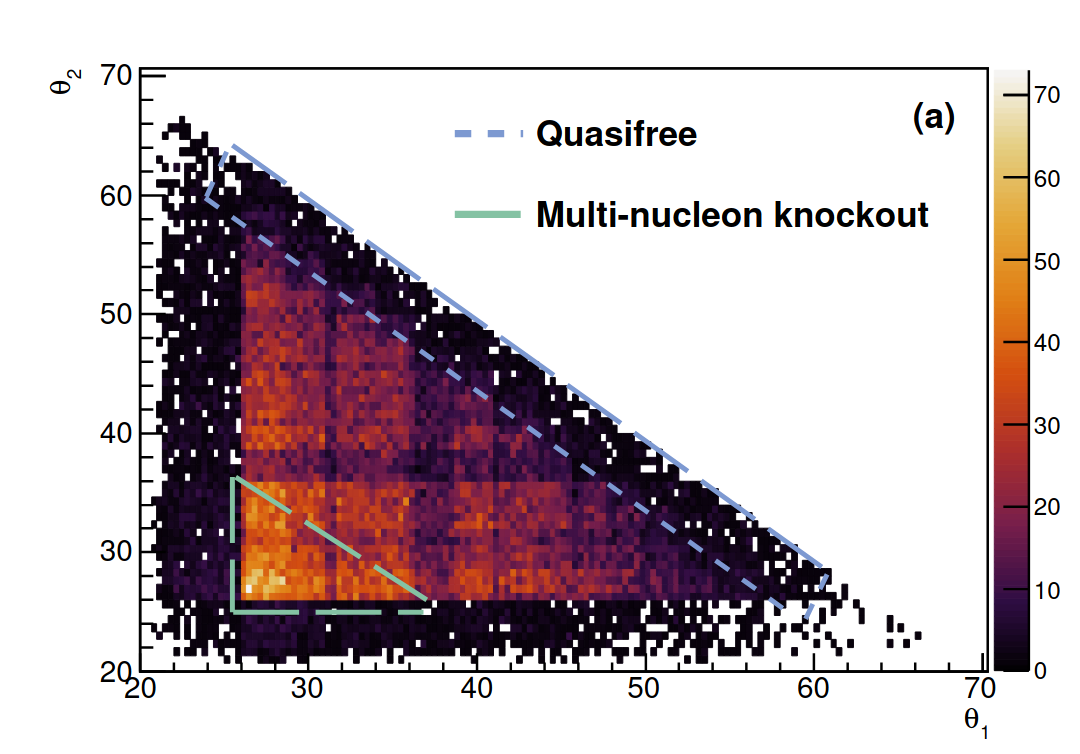
\includegraphics[width=\textwidth]{Figures/gabriel_1.png} 
    \end{subfigure}
    \begin{subfigure}[b]{0.3\textwidth}
    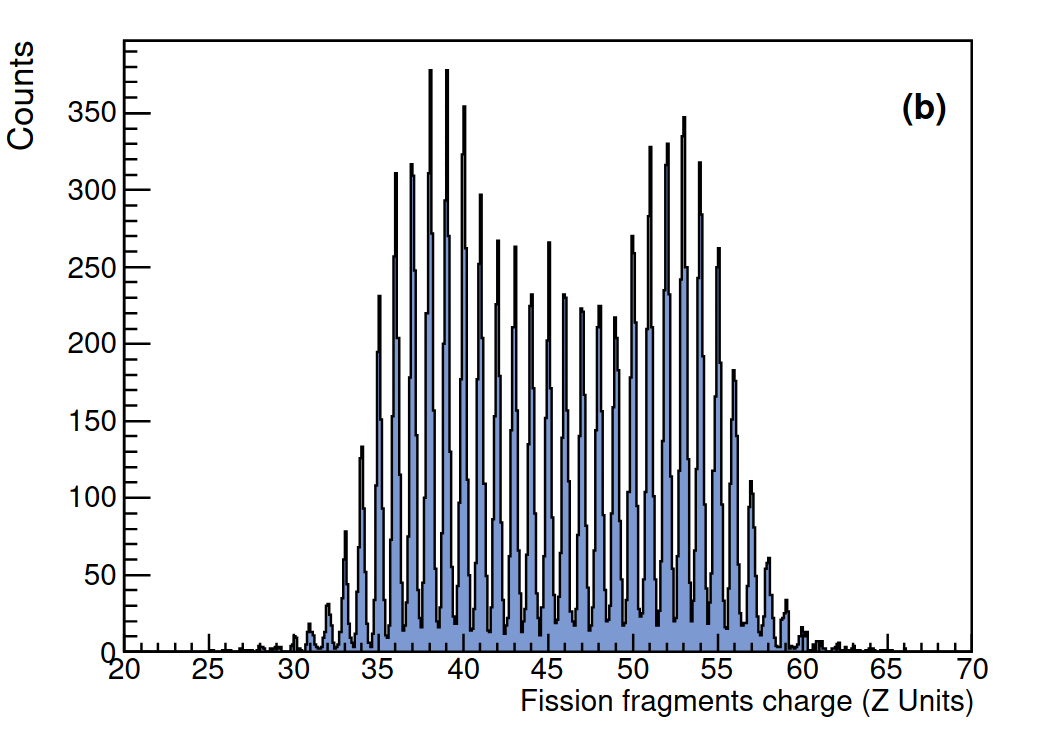
\includegraphics[width=\textwidth]{Figures/gabriel_2.png} 
    \end{subfigure}
    \begin{subfigure}[b]{0.3\textwidth}
    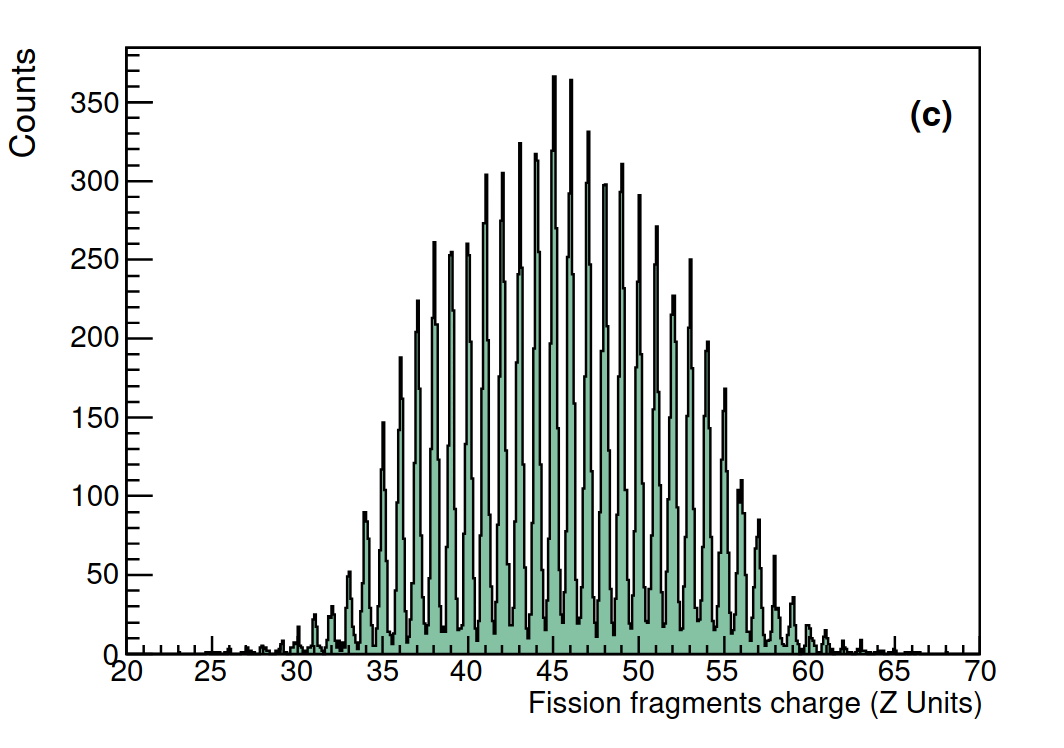
\includegraphics[width=\textwidth]{Figures/gabriel_3.png}
    \end{subfigure}
    \caption{(a) Polar angle correlations of the two protons from fission via QFS event. In (b)  the charge distribution for quasi-free (p,2p) fission reactions is selected while (c) displays the charge distribution for multi-nucleon knockout reactions of FSI. From Ref \cite{garcia2023study}, S455 Experiment in 2021 at R$^3$B, GSI.}
    \label{fig:qfs_fission}
\end{figure}

\end{description}

\newpage\null\thispagestyle{empty}\newpage
\section{Experiment}
The present commissioning experiment was performed in 2020 at the FAIR Facility at GSI (Gesellschaft f\"ur Schwerionenforschung) in Darmstadt (Germany). The GSI Helmholtzzentrum für Schwerionenforschung operates a unique accelerator facility for heavy ions and focuses on several cutting-edge research fields. These include:\newline
\begin{enumerate}
\item \textbf{Nuclear Physics}: Studying the properties of atomic nuclei, exploring the forces that bind protons and neutrons, and investigating exotic nuclei far from stability.
\item \textbf{Hadron and Quark Matter}: Investigating the behavior of hadrons (particles made of quarks) and the state of matter under extreme conditions, such as those found in neutron stars or during the early universe.
\item \textbf{Atomic Physics}: Examining the structure and dynamics of atoms, including highly charged ions, to understand fundamental atomic interactions and refine quantum electrodynamics.
\item \textbf{Plasma Physics}: Creating and analyzing high-energy-density plasmas to simulate conditions found in stellar interiors and other astrophysical phenomena.
\item \textbf{Biophysics and Medical Research}: Exploring the effects of ion beams on biological systems for applications in cancer therapy, particularly using heavy ion therapy, and studying radiation protection for space missions.
\item \textbf{Materials Research}: Investigating the response of materials to high radiation doses to develop more resilient materials for use in various technologies, including nuclear reactors and space exploration.
\end{enumerate}
\subsection{GSI facility}
The GSI Helmholzzentrum f\"ur Schwerionenforschung located at Darmstadt has a long history of research.... tell something about the beginnnings, first really heavy elements found there.\newline
%Tell about the central apparatus: Linear Accelerator UNILAC, Ring Accelerator SIS 18, FRS,  and the different experimental halls, see: https://web.archive.org/web/20141222164000/https://www.gsi.de/en/research/accelerator_facility.htm?nr=%2Fproc%2Fself%2Fe
The GSI Helmholtzzenrum f\"ur Schwerionenforschung GmbH was founded in 1969 (as "Gesellschaft f\"ur Schwerionenforschung mbH) looks back on a successful research history. In the time between 1981 and 2010 six new  superheavy elements were discovered. \newline
In the medical research field GSI has developed advanced cancer therapy techniques using heavy ion beams which target tumors with high precision, minimizing damage to surrounding healthy tissues.\newline
Along with those groundbreaking discoveries in research the facility at GSI has always been an inspiring source of drive for new technologies.\newline
The key devices/apparatus which enable to carry out experiments with heavy ions at GSI are:
%cite from:
%https://www.gsi.de/en/researchaccelerators/accelerator_facility
important to mention: GSI is the only facility with heavy ions in the world
The starting point for the production of relativistic heavy ions at GSI is the ion source where ions are generated by stripping electrons off the shell of the atoms. Depending on the experimental needs the ion sources at GSI are able to produce ions of many different kinds of elements (up to Uranium).\newline
%cite here: https://www.gsi.de/en/researchaccelerators/accelerator_facility/ion_sources
On the first acceleration stage the stable primary ions are injected from the ion source into the UNIversal Linear Accelerator (UNILAC). On a length of 120 meters ions are accelerated up to maximum energy of 11.4 AMeV. The low energy beam is now injected into the ring accelerator SIS18 (Schwerionensynchotron 18). Here the ion beam is further accelerated up to 4.7 GeV/u (for protons) / 1 GeV/u (for Uranium). The magnets and  the ultra-high vacuum (~ 10⁻9 Pa) keep the ions well on their circular path (SIS18 has a circumference of 216 meters). For the production of rare heavy isotopes the primary ion beam from SIS18 can be impinged on a light nuclear target, e.g beryllium, the so called production target. These secondary beams of radioactive isotopes can be either stored in the experimental storage ring (ESR) for later use or transferred to the FRagment Separator (FRS). The FRS as a high-resolution magnetic spectrometer is capable to precisely select specific isotopes and to forward the desired beam of exotic relativistic nuclei to the various experiments or direct it to the ESR for later use.\newline
%cite here: https://www.gsi.de/en/researchaccelerators/accelerator_facility/ring_accelerator
\subsubsection{FAIR Project}
The FAIR (Facility for Antiproton and Ion Research) situated next to the GSI will be one of the most complex and largest accelerator facilities in the world. The construction of the superconducting ring accelerator SIS100 with a circumference of 1.1 km, storage rings and experiment sites begun in the summer of 2017. Commissioning is planned in 2025 (?). Early Science. 
\subsection{R3B Setup}
\subsubsection{Detector Setup in S444 Commmissioning Experiment 2020}
\subsubsection{Calibration of the Detector Systems}




\section{Analysis - Total Interaction Cross Section of  $^{12}$C + $^{12}$C}
This chapter will go through the  analysis step by step from the unpacking stage to the final measurement of the total interaction cross section. It will start by a short overview of the transmission method used for the cross section measurements. The next step is  the selection of clean incoming $^{12}$C isotopes. Following the identification of the carbon isotopes after the target - for the measurement of the charge changing cross section - and as final step the interaction cross section measurement. \newline
All relevant detector related geometrical and efficiency corrections will be adressed and their influence to the final result and its uncertainty will be discussed.
\subsection{Cross Section Measurement via Transmission Method}\label{section:transmission_method}
In its most generic form cross sections give a measure of the probability that a specific reaction will take place when two or more particles collide. The cross sections  measured in scattering exepriments, as well as the energy and angular distribution of the reaction products, provide information about the dynamics of the interaction between the projectile and the target particle, i.e., about the shape of the interaction potential and the coupling strength.\newline
The cross section $\sigma$ can be derived by looking at the relation between the number of incoming particles (N$_{1}$) and unreacted particles after the target ($N_{2}$). For an experiment with fixed target with thickness $z$ and volumetric number density $n$ the number of reacted particles in the infinitesimal thin target layer $dz$ can be expressed as:
\begin{equation}
\frac{dN_{2}}{dz} = -n \sigma N_{2}
\end{equation}
Solving this differential equation for $N_{2}$ (with the condition $N_{2}$ = $N_{1}$ for $z=0$) discloses an exponential relation:
\begin{equation}
N_{2} = N_{1}e^{-n\sigma z}  = N_{1}e^{-N_t\sigma}
\label{eq:cross_sec}
\end{equation} 
Where $n\cdot z$ can be summarized as $N_t$, the total number of scattering centers per unit area. The relation $(N_{2}/N_{1})$, number of unreacted particles after the target versus number of incoming particles, is often called survival probability. For an idealistic experimental setup with full detector efficiency and no interactions in the setup material the cross section could simply be deduced from equation \ref{eq:cross_sec}. To account for reactions of the projectile that occur within the setup material and first order detector specific distortions of output signals the survival probabiltiy $(N_{2}/N_{1})$ has to be divided by $(N_{2}^E/N_{1}^E)$, where $N_{1}^E$ is the number of incoming particles and $N_{2}^E$ the number of unreacted particles after the target for an empty run respectively. Thereby the setup specific efficiency($\epsilon_{setup}$) and transmission factor($t_{setup}$) are cancelled out to obtain the underlying number of unreacted particles after the target $\tilde{N_{2}}$:\newline
$N_{2} = \tilde{N_{2}} \cdot t_{setup}\cdot \epsilon_{setup}$, with $\tilde{N_{2}}$\newline
$N_{2}^E = \tilde{N_{2}^E} \cdot \epsilon_{setup}$ with $\frac{\tilde{N_{2}^E}}{N_{1}^E}$ the setup specific transmission factor $t_{setup}$ \newline
\newline
The final formula for the cross section for a so called transmission measurement is:
\begin{equation}
	\begin{split}
\sigma = -\frac{1}{N_t} ln(\frac{N_{1}^E}{N_{2}^E} \cdot \frac{N_2}{N_1}) = -\frac{1}{N_t} ln(\frac{N_{1}^E}{\tilde{N_{2}^E} \cdot t_{setup}\cdot \epsilon_{setup}} \cdot \frac{\tilde{N_{2}^E} \cdot \epsilon_{setup}}{N_1}) \\
\text{With $\frac{\tilde{N_{2}^E}}{N_{1}^E} = t_{setup}$} \\
\sigma = -\frac{1}{N_t} ln(\frac{1}{t_{setup}} \cdot \frac{\tilde{N_{2}} \cdot t_{setup}}{N_1}) = -\frac{1}{N_t} ln(\frac{\tilde{N_{2}}}{N_1})
\label{eq:corr_cross}
	\end{split}
\end{equation}
From the above formula \ref{eq:corr_cross} it is evident that for cross section measurements with the transmission method three types of observables have to be measured:\newline
\begin{enumerate}
\item[$\blacksquare$] \textbf{Number of scattering centers $\mathbf{N_t}$}\newline
The number of scattering centers per unit area of the target is a target specific number. It depends from the target thickness and and its density. The values herefore are taken from \cite{ponnath2023precise}\footnote{For the purpose of this work the target thicknesses were remeasured at GSI with a chromatic sensor giving 2D depth profiles of each target.}:
\begin{enumerate}
\item Thin target:\newline 
target thickness d = 0.5451 cm; $N_t = 5.0588795\cdot 10^{22}$; $\Delta N_t = 0.0648\%$
\item Medium target:\newline
target thickness d = 1.0793 cm; $N_t = 1.0016600\cdot 10^{23}$; $\Delta N_t = 0.2620\%$
\item Thick target:\newline
target thickness d =2.1928cm; $N_t = 2.0350598\cdot 10^{23}$; $\Delta N_t = 0.0322\%$
\end{enumerate} 
where $N_t$ was calculated by:
\begin{equation}
N_t = \frac{\rho \cdot d \cdot N_A}{M}
\end{equation}
with $\rho$ the target density\footnote{$\rho = 1.851 g/cm^{3}$, from \cite{ponnath2023precise}}, $N_A$ the Avogadro constant ($6.02214076\cdot10^{23}\,mol^{-1}$) and $M$ the molar mass of the target (for carbon $M = 12.011g \cdot mol^{-1}$).
\item[$\blacksquare$] \textbf{Number of incoming projectiles ($^{12}$C) $\mathbf{N_1}$}\newline
For the measurement only events with well identified incoming $^{12}$C projectiles are chosen. Herefore strict cuts on the detectors upstream the target area are set. This strict event selection makes sure that we only consider events with single $^{12}$C. This will be discussed in more detail in section \ref{subsec:event-sel}.  %TODO finish this sencence 
\item[$\blacksquare$] \textbf{Number of unreacted projectiles ($^{12}$C) $\mathbf{N_2}$ after the target}\newline
Detectors downstream the target area are used to count the number of unreacted projectiles $^{12}$C. To reduce detector specific influences which could distort the result it is advisable to use only as few as requirable detectors for the clear identification of unreacted projectiles. Moreover detector specific efficiencies are cancelled out by including both empty and target runs in the cross section calculation(see equation\ref{eq:corr_cross}). For all downstream detectors used in this analysis it is critical to minimize any selection cuts and systematically check their effects on $N_2$.
\end{enumerate}
\subsection{Event Selection}\label{subsec:event-sel}
\begin{figure}[htpb]
    \centering
    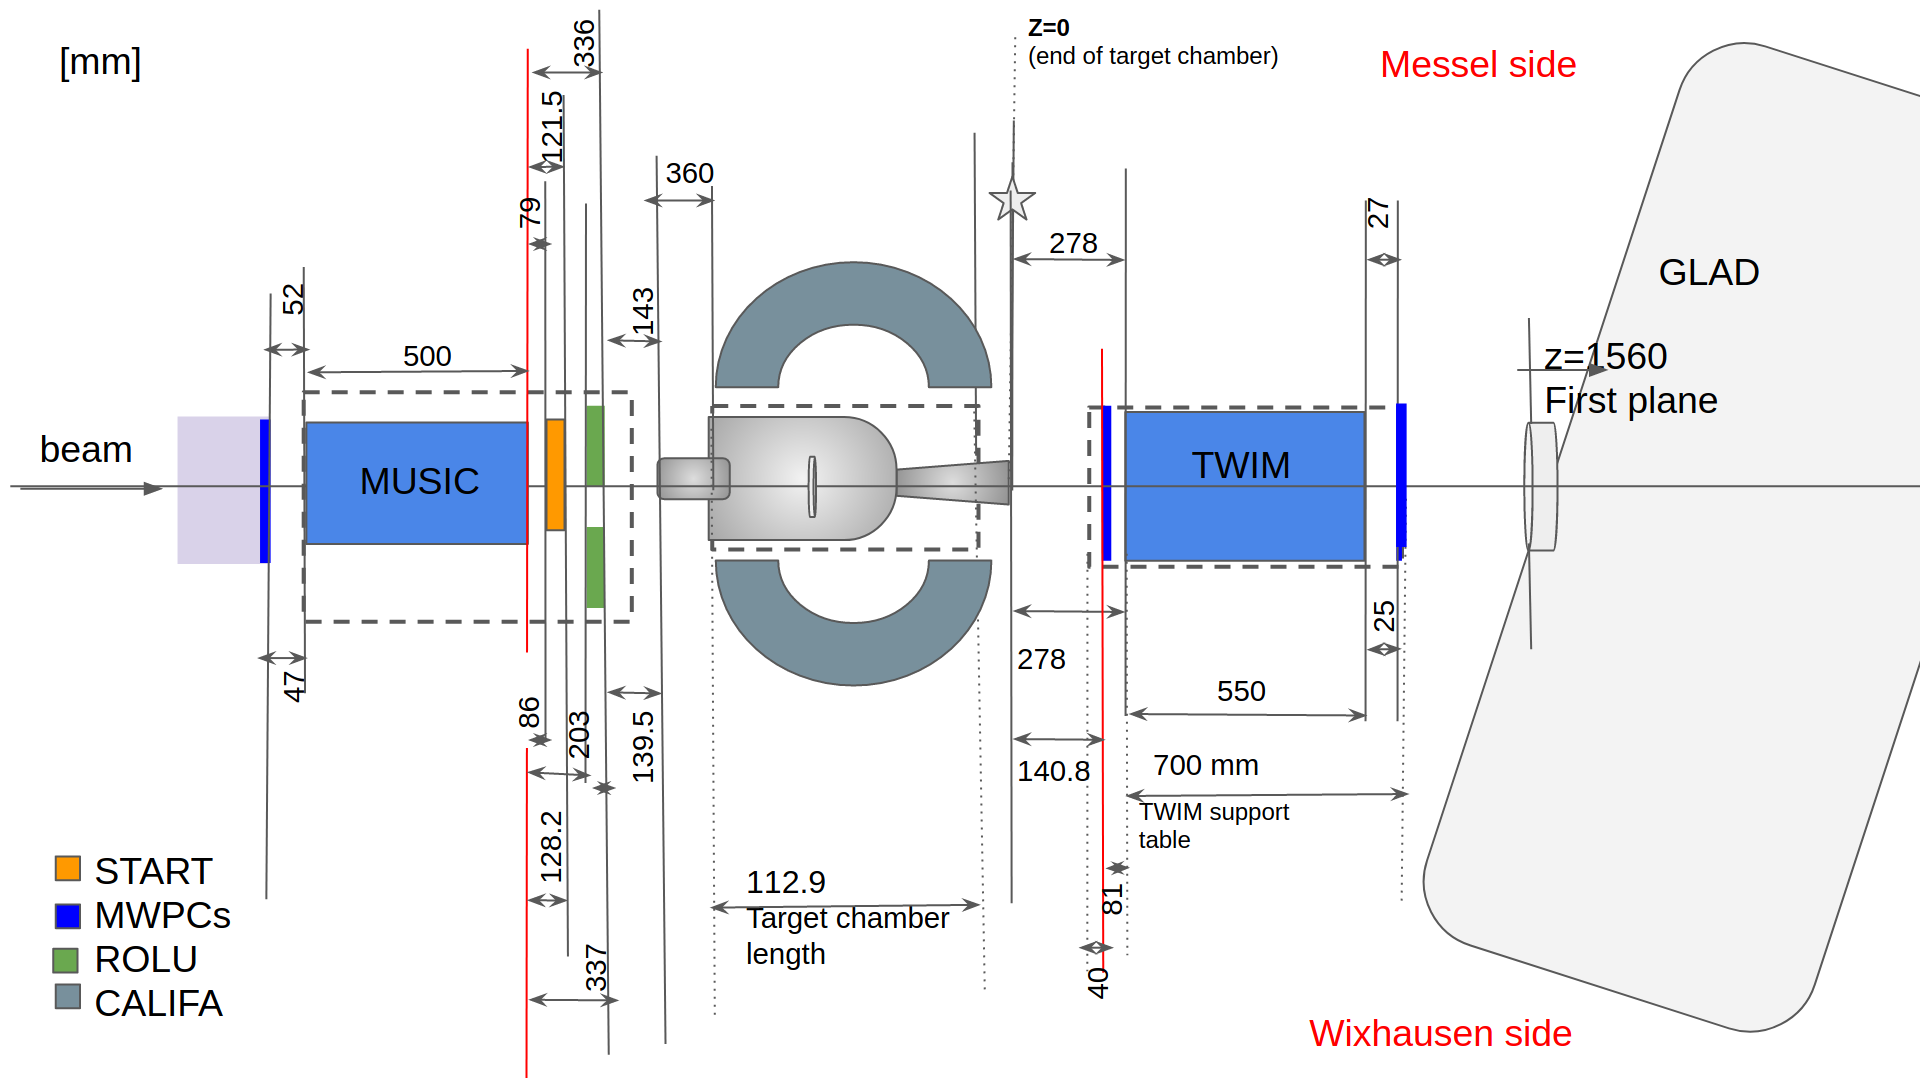
\includegraphics[width=\textwidth,height=6cm,keepaspectratio=true]{Figures/SETUP_around_Target.png}
    \caption{
    R3B Setup for the S444 experiment in the target region. TODO: select overview with less numbers/measures...
    }
    \label{fig:setup_target_region}
\end{figure}

For event selection, all three upstream detectors are utilized: the MWPC0, the R3BMUSIC Ionization Chamber, and the start detector. To ensure a clean incoming event selection, the following prerequisites must be met:
\begin{enumerate}
\item \textbf{$^{12}$C identification of incoming projectile by upstream detectors:}\newline
\begin{figure}[htpb]
    \centering
    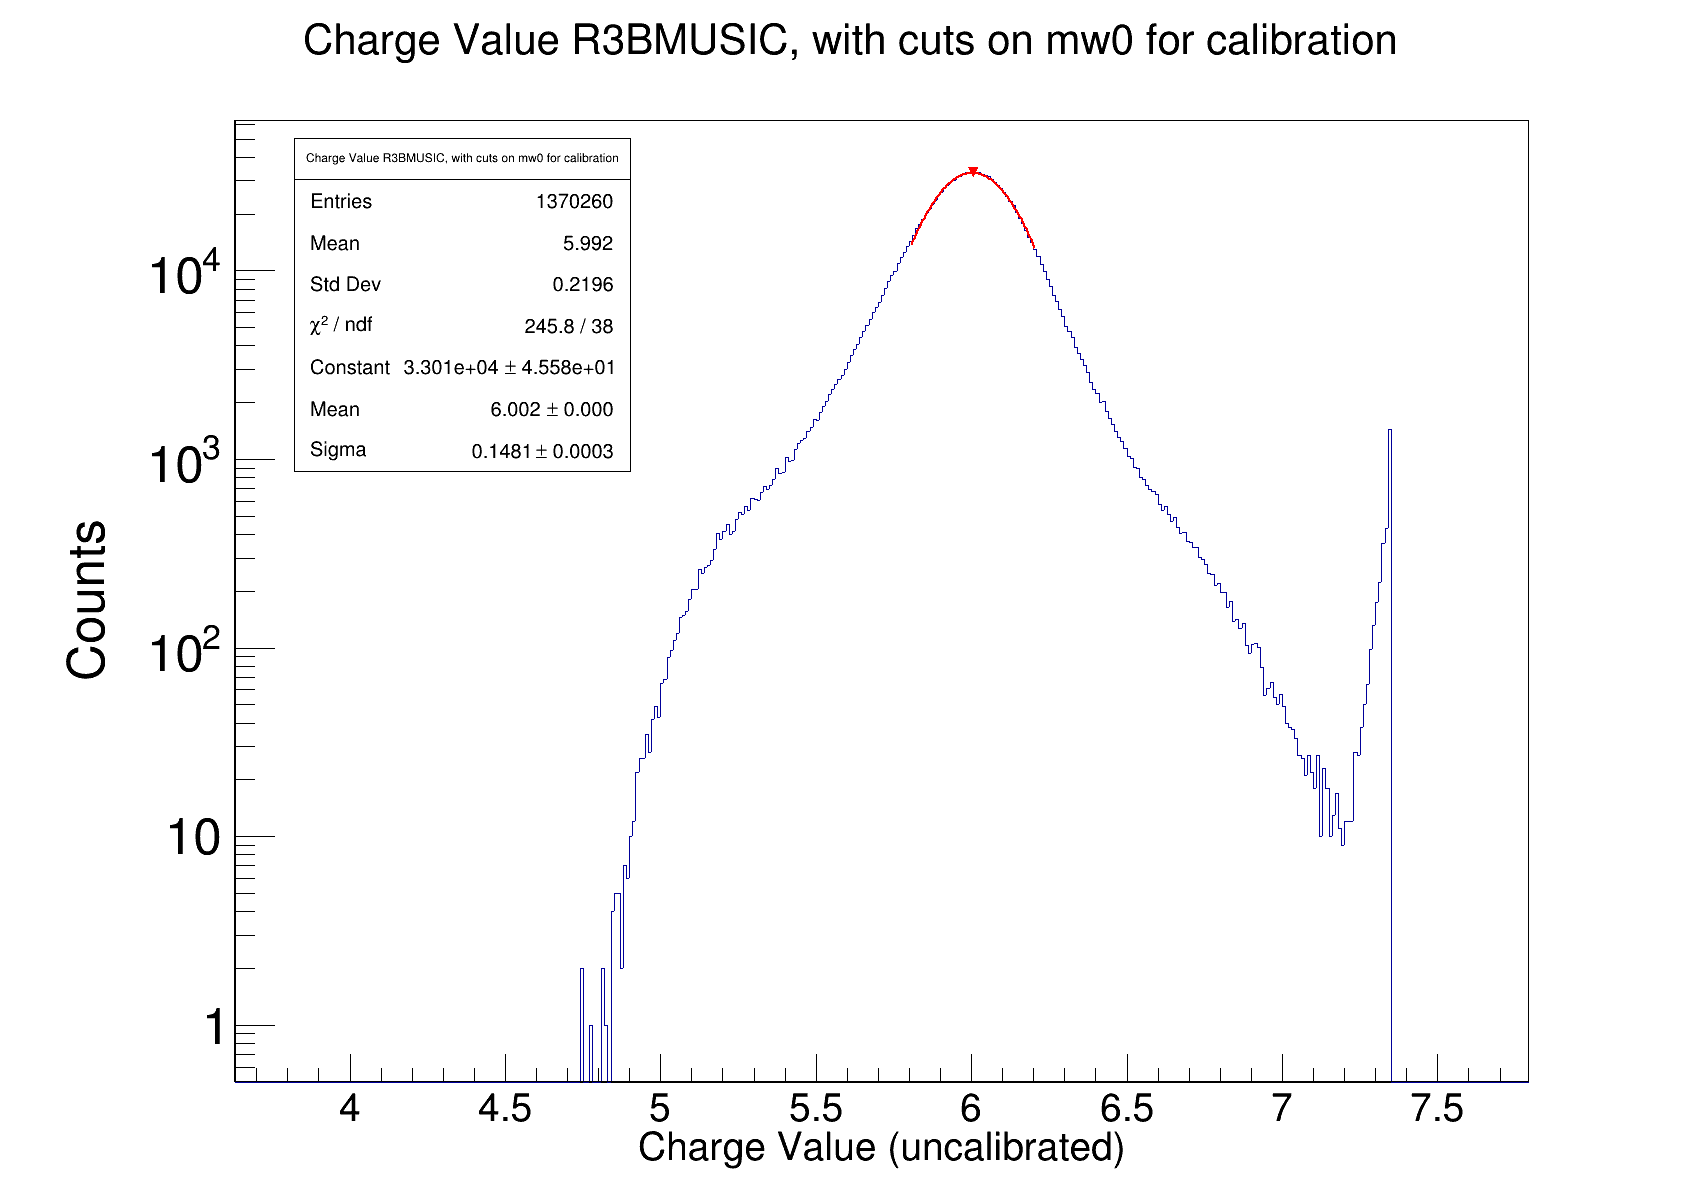
\includegraphics[width=\textwidth,height=8cm,keepaspectratio=true]{Figures/charge_r3bmusic.png}
    \caption{
    Charge distribution on R3BMUSIC with predefinded calibration parameters with already applied positional cuts on MWPC0 - positioned upstream to the ionisation chamber. The rise beyond Z $\ge$ 7.2 comes from pile-up events. TODO: more explanation needed? 2D plot needed? 
    }
    \label{fig:r3bmusic_charge}
\end{figure}
In the S444 experiment the incoming beam was directly delivered by the SIS18 ring accelerator, which is operated in ultra-high vacuum.The level of contamination is low.(TODO:up to which stage do we have vacuum? Until MW0?)\newline %TODO:up to where is the beam in vacuum?
For the charge identification of the incoming ion the R3BMUSIC ionisation chamber is used which is positioned directly after the MWPC0 at the beam entrance in Cave C, see figure \ref{fig:setup_target_region}. The R3BMUSIC detector measures anode-wise the energy loss of the passing-through ion which in the first order is proportional to the square of its charge ($\Delta E \sim Z^{2}$). Herfore the calibration parameters from the online analysis are used\footnote{These are generic paramteter values used to the detector performance during the experiment phase.}. Figure \ref{fig:r3bmusic_charge} shows the measured charge distribution in R3BMUSIC. To select $Z = 6$ incoming ions the distibution is fitted with a gaussian fit function. All ions with charge within the $\pm 1 \sigma$ range are accepted. Figure \ref{fig:r3bmusic_cuts} summarizes the $\pm 1 \sigma$ cuts on the R3BMUSIC charge for empty/target runs for all beam energies.   
\begin{figure}
\centering
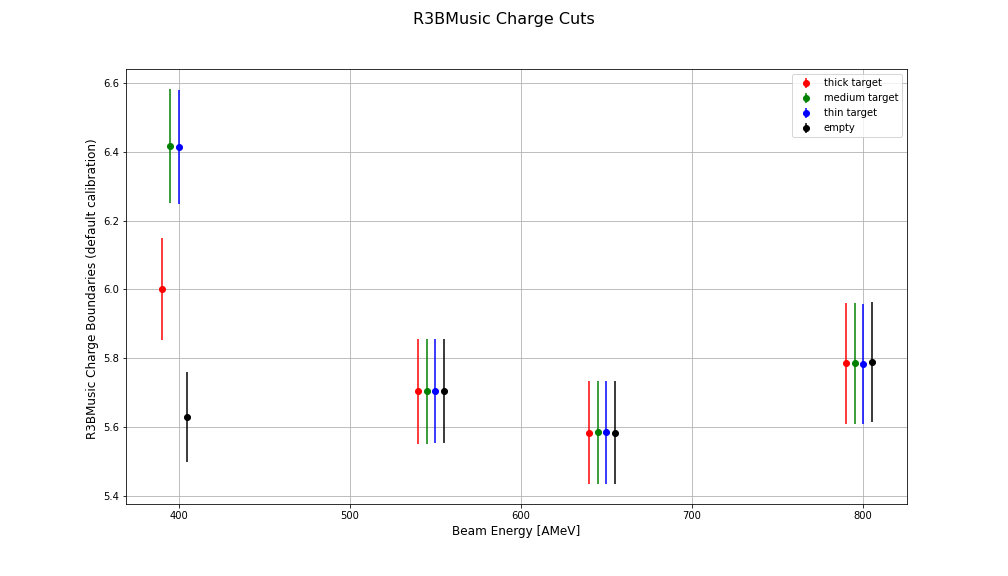
\includegraphics[width=\textwidth,height=8cm,keepaspectratio=true]{Figures/r3bmusic_charge_cuts.png}
\caption{Strict $\pm 1 \sigma$ charge cuts with R3BMUSIC for incoming particle selection. Fixed predefined calibration parameters were used which do not compensate different gain settings between runs. This is in particular the case for the 400 AMeV beam energy runs.}
\label{fig:r3bmusic_cuts}
\end{figure}
\item \textbf{Pileup rejection and TPat selection:}\newline
The overall recoding and merging of the data from various subdetectors is one of the tasks of the Data AcQuisition (DAQ) system. Whether an event is recorded or not depends on the pre-established trigger logic. Various detectors can send out triggers to the main DAQ when certain conditions are given (e.g. CALIFA can be configured to send out a trigger when a hit with more than 20 MeV is recorded in the calorimeter). The different triggers are processed by the trigger logic and summarized as a defined trigger pattern, so called TPat, which is stored in a 16-bit mask for each event. Table \ref{tab:tpats} gives an overview of the trigger logic and the trigger patterns set in the S444 experiment. For this analysis the \textit{"Min. Bias"} trigger is required\footnote{This includes also \textit{"Reaction"} and \textit{"Neutron"} TPat since these patterns contain also \textit{"Min. Bias"} TPat as necessary condition.}.\newline 
\begin{table}[h!]
\centering
\begin{tabular}{||c c c||} 
\hline
Bit Position &TPat Name & Description \\
\hline\hline
0 & Min Bias & Hit in Start detector\\
1 & Reaction & "CalifaOR" -high energy hit in CALIFA \\
2 & Neutron & Hit in NeuLAND \\
3 & p+n & Hit in CALIFA and Neuland \\
8 & Califa & high energy hit in califa - off-spill \\
9 & NeuLAND & Hit in NeuLAND - off-spill \\
\hline\hline
\end{tabular}
\caption{List of TPats set for S444 experiment. As for the selected runs low beam rates ($< 10kHz$) were expected no dead time issues should arise for the in-beam detectors, therefore no downscaling of the \textit{Min. Bias} TPat was deployed.}
\label{tab:tpats}
\end{table}
Since the TPat selection itself does not necessary set any pileup constraints it is important to analyse the signals of the detectors upstream carefully to insure yourself that only events with  one incoming $^{12}$C ion at a time get selected. Herefore events with incoming ions with charge $Z = 6 \pm 1\sigma$ are chosen, as discussed in the previous point. Moreover it is required that both left and right preamplifiers of the start detector have seen a coincident signal within a time-window of 1.391 ns.---TODO: why this time window?-- The overall searching window of the start detector was set to 2 $\mu s$, see figure \ref{fig:start_good_event_sel}. For the MWPC0 which is mounted right at the beam entrance of Cave C no hit multiplicity cuts were applied considering its operating mode, which is designed for charge sharing between the readout pads. 
\begin{figure}
\centering
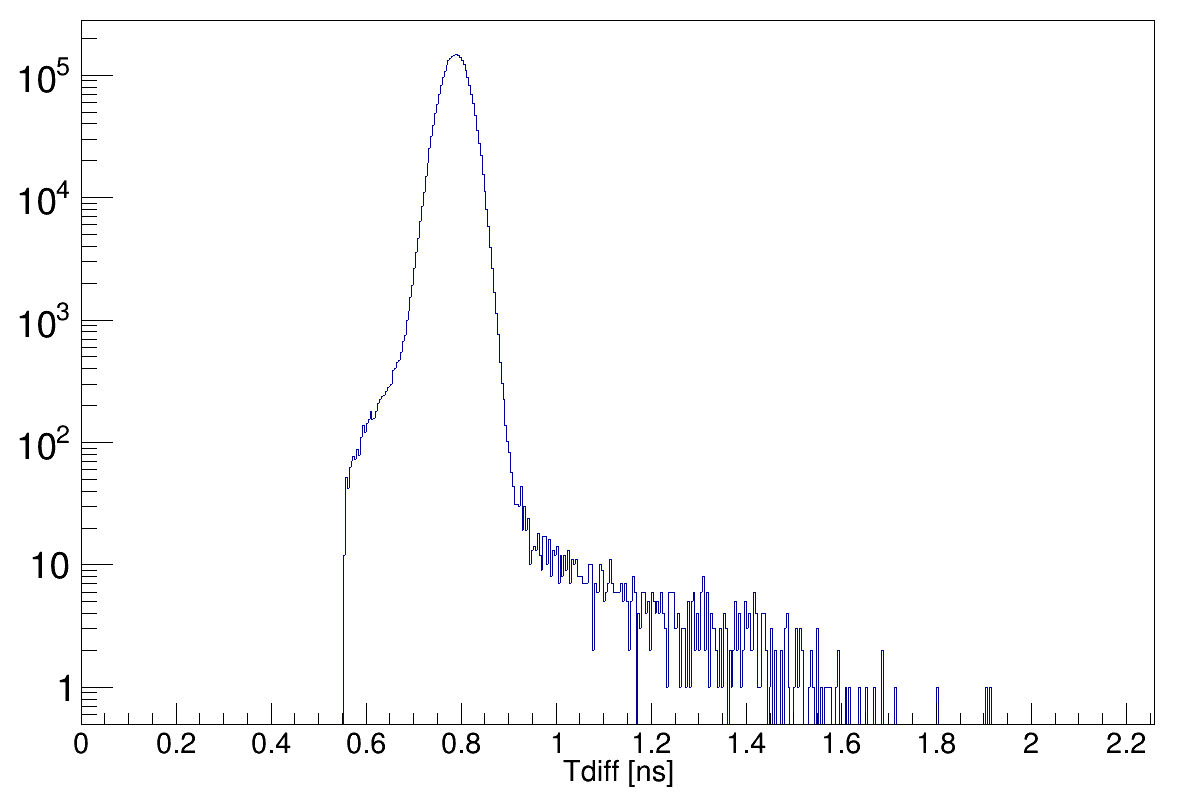
\includegraphics[width=\textwidth,height=8cm,keepaspectratio=true]{Figures/start_tdiff_exactly2good_hits.png}
\caption{$\Delta t_{right-left}$ between hits in the Start detector for events with exactly one hit on the left and right preamplifier and limiting the time differnce in the range 0.555 ns to 1.946ns.}
\label{fig:start_good_event_sel}
\end{figure}
\item \textbf{Projectile's focus on the active target region:}\newline
To assure that the incoming $^{12}$C ion hits the target it is necessary to select only events where the projectile is focussed to the active target region. Therefore strict cuts on the MWPC0 x and y positon are applied. This was achieved by fitting the x and y distribution of the MWPC0 (without any restrictions on it) by a gaussian function. The selection of focused incoming projectiles was then restricted to events with hits in MWPC0 within the $\pm 1\sigma$ region in the x and y position, see figure \ref{fig:mw0_xy_overview} and \ref{fig:mw0_cuts}.\newline
\begin{figure}
\centering
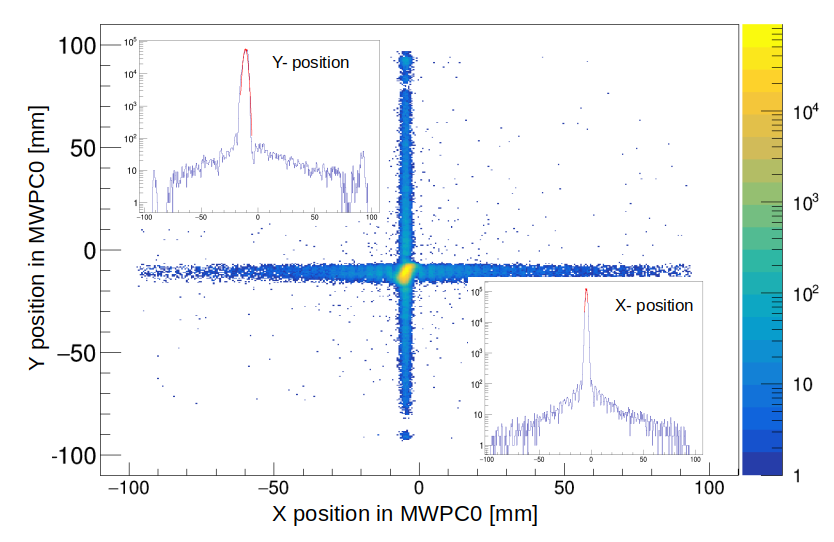
\includegraphics[width=\textwidth,height=8cm,keepaspectratio=true]{Figures/mw0_xy_summary.png}
\caption{x-y position of incoming ion on MWPC0.}
\label{fig:mw0_xy_overview}
\end{figure}
\begin{figure}
\centering
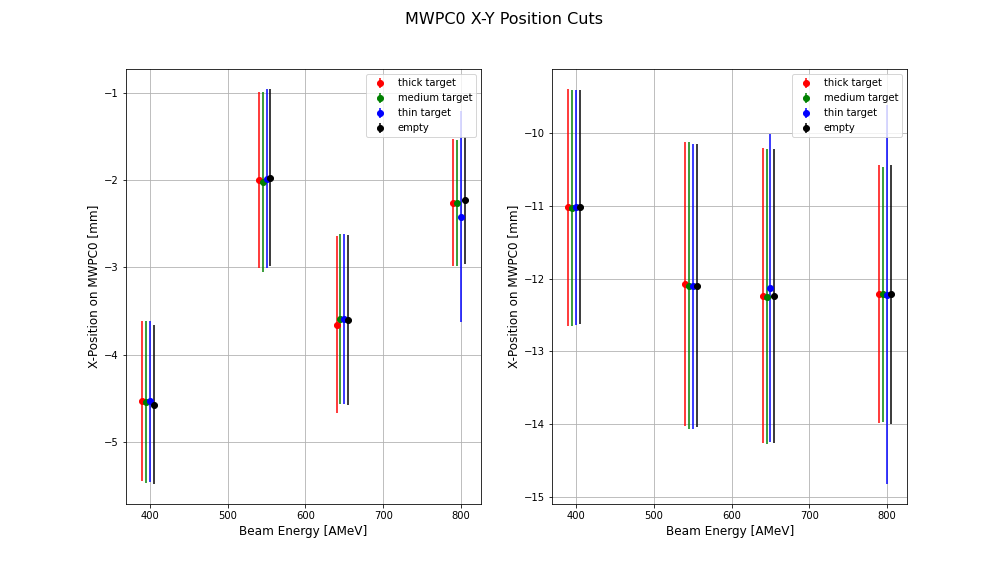
\includegraphics[width=\textwidth,height=8cm,keepaspectratio=true]{Figures/mwpc0_cutxy.png}
\caption{Overview of $\pm 1\sigma$ cuts in x and y in MWPC0 for empty/target runs. TODO: labelling on the right side is wrong! (should be y!)}
\label{fig:mw0_cuts}
\end{figure}
The MWPC0 x-position and the available projectile angle in the x-y plane from the R3BMUSIC is used to propagate the corresponding x-position on the target location to further check that the selected projectiles hit the target parallel to the z-position (= beam direction) and do only have a minimal incident angle, see figure \ref{fig:x_pos_target}. 
%This can also be seen as a consistency check whether the applied (predefined) calibration parameters are properly set.
\begin{figure}[htpb]
    \centering
    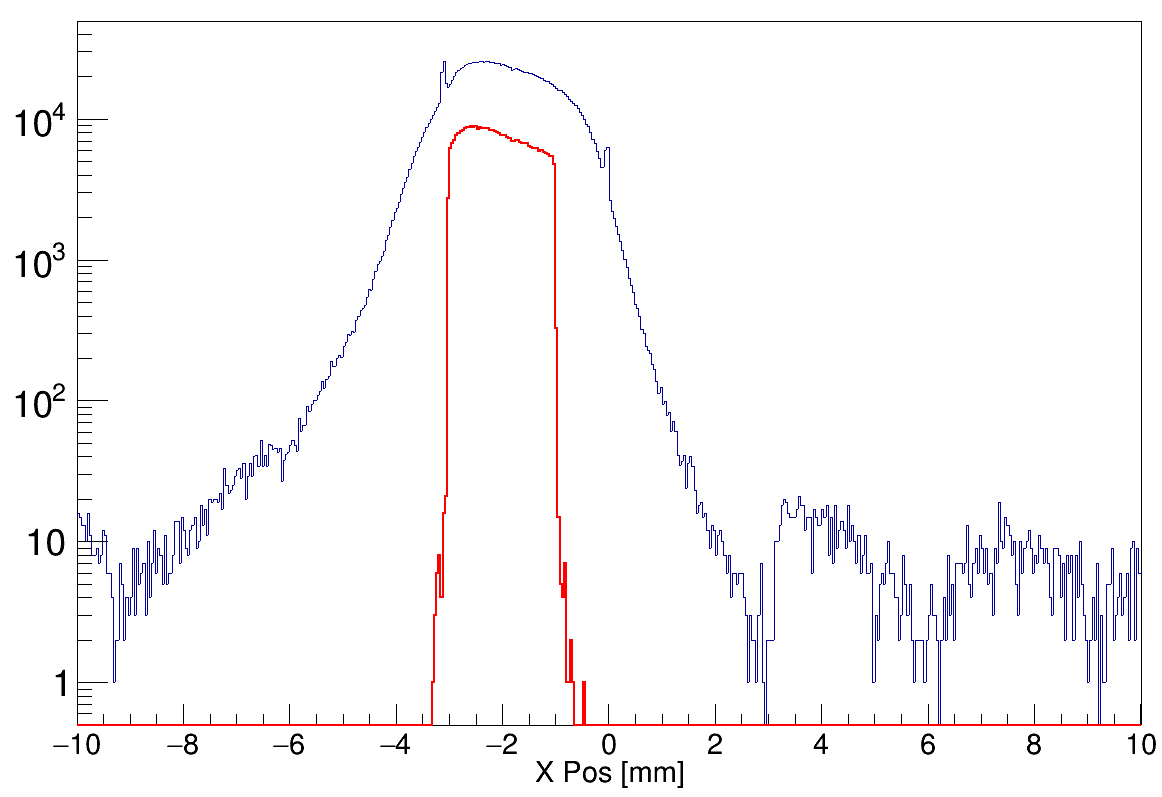
\includegraphics[width=\textwidth,height=8cm,keepaspectratio=true]{Figures/x_proj_beam_mw0_target.png}
    \caption{
   	Propagated x-position on target location from measured x-value on MWPC0 and x-y plane angle measurement from R3BMUSIC. The target area is 3 x 3 cm. In red the selected events with $\pm 1\sigma$ cut in x and y position in MWPC0, in blue all events. TODO: which run is this?
    }
    \label{fig:x_pos_target}
\end{figure}
\end{enumerate}
\subsection{Charge Changing Cross Section Measurement}\label{subsec:cc_cs}
The charge changing cross section refers to a measure of the probability that the incoming projectile will undergo a reaction inside the target that changes its charge. To measure the charge changing cross section it can be referred to formula \ref{eq:corr_cross} where in this case $N_2$ is the number of survived carbon isotopes, i.e. projectiles which did not change their charge state. For this measurement only the data from the double ionisation chamber TWIN Music (see section \ref{sec:ionisation_chambers}) needs to be read out and analyzed.\newline
While for the event seletion before the target the cut conditions can be arbitrarly strict (it will only have an impact to the statistics and the derivated statistical error), cuts on the downstream detectors need to be avoided if at all possible. Too selective cuts on the identification of $N_2$ can distort the measurement.
\subsubsection{TWIN MUSIC Calibration}
For the analyis of data in TWIN MUSIC - different to the upstream detectors, where calibrated data with default calibration parameters is used - the so called \textit{mapped} raw level data is processed. In the mapped level TWIN MUSIC provides following information:
\begin{itemize}
\itemsep0em 
\item \textbf{SectionID:} The detector is a double ionisation chamber and as such divided into four parts (in beam perspective): section 1 - right down; section 2 - right up; section 3 - left down; section 4 - left up. For the S444 experiment only section 1 was operated and accordingly centered on the beam spot.
\item \textbf{AnodeID:} TWIN MUSIC has 16 anodes for energy-loss readout and one refence anode (anodeID = 17).
\item \textbf{Time:} Each hit in each anode gets assigned to a time. Each time has individually no meaning. The drift time (in ns) of the electrons from the ionisation process of the gas by the inflying projectile (or the fragments of it) to the anode is calculated by substracting the individual anode time by the time of the reference anode. The reference anode receives its clean signal from a constant fraction discriminator of the start detector.
\item \textbf{Energy:} Each hit in each anode gets assigned to an energy - except the hit in the reference anode. To reconstruct the charge of the crossing through charged particle anodewise or detectorwise the parmetrization formula Z = [0] + [1]*$\sqrt(E)$ + [2]*E is used. 
\end{itemize}
The calibration of the TWIN energy for each anode is done run-wise. 
%The event selection on the incoming ion is limited to the  \textit{"Min. Bias"}-TPat condition (coincident signal in start detector preamplifiers within 1.391 ns, on-spill).
For the TWIN MUSIC only events where all anodes having exactly one hit (including the reference anode) are chosen. The most prominent peak (Z = 6) was fitted with gaussian function. The calibration was then done by determining the scaling factor for each anode  that shifts the mean of the gaussian fits to the same position, see figure \ref{fig:calibration}. For this analysis the peaks were shifted to $\Delta E = 6$. Since $\Delta E \propto Z^2$ holds, the scaled $\Delta E$ value, even though peaking at 6, is not equate the charge Z = 6.
TODO: describe better the calibration steps!!! this is not good!
\begin{figure}
     \centering
     \begin{subfigure}[t]{0.45\textwidth}
         \centering
         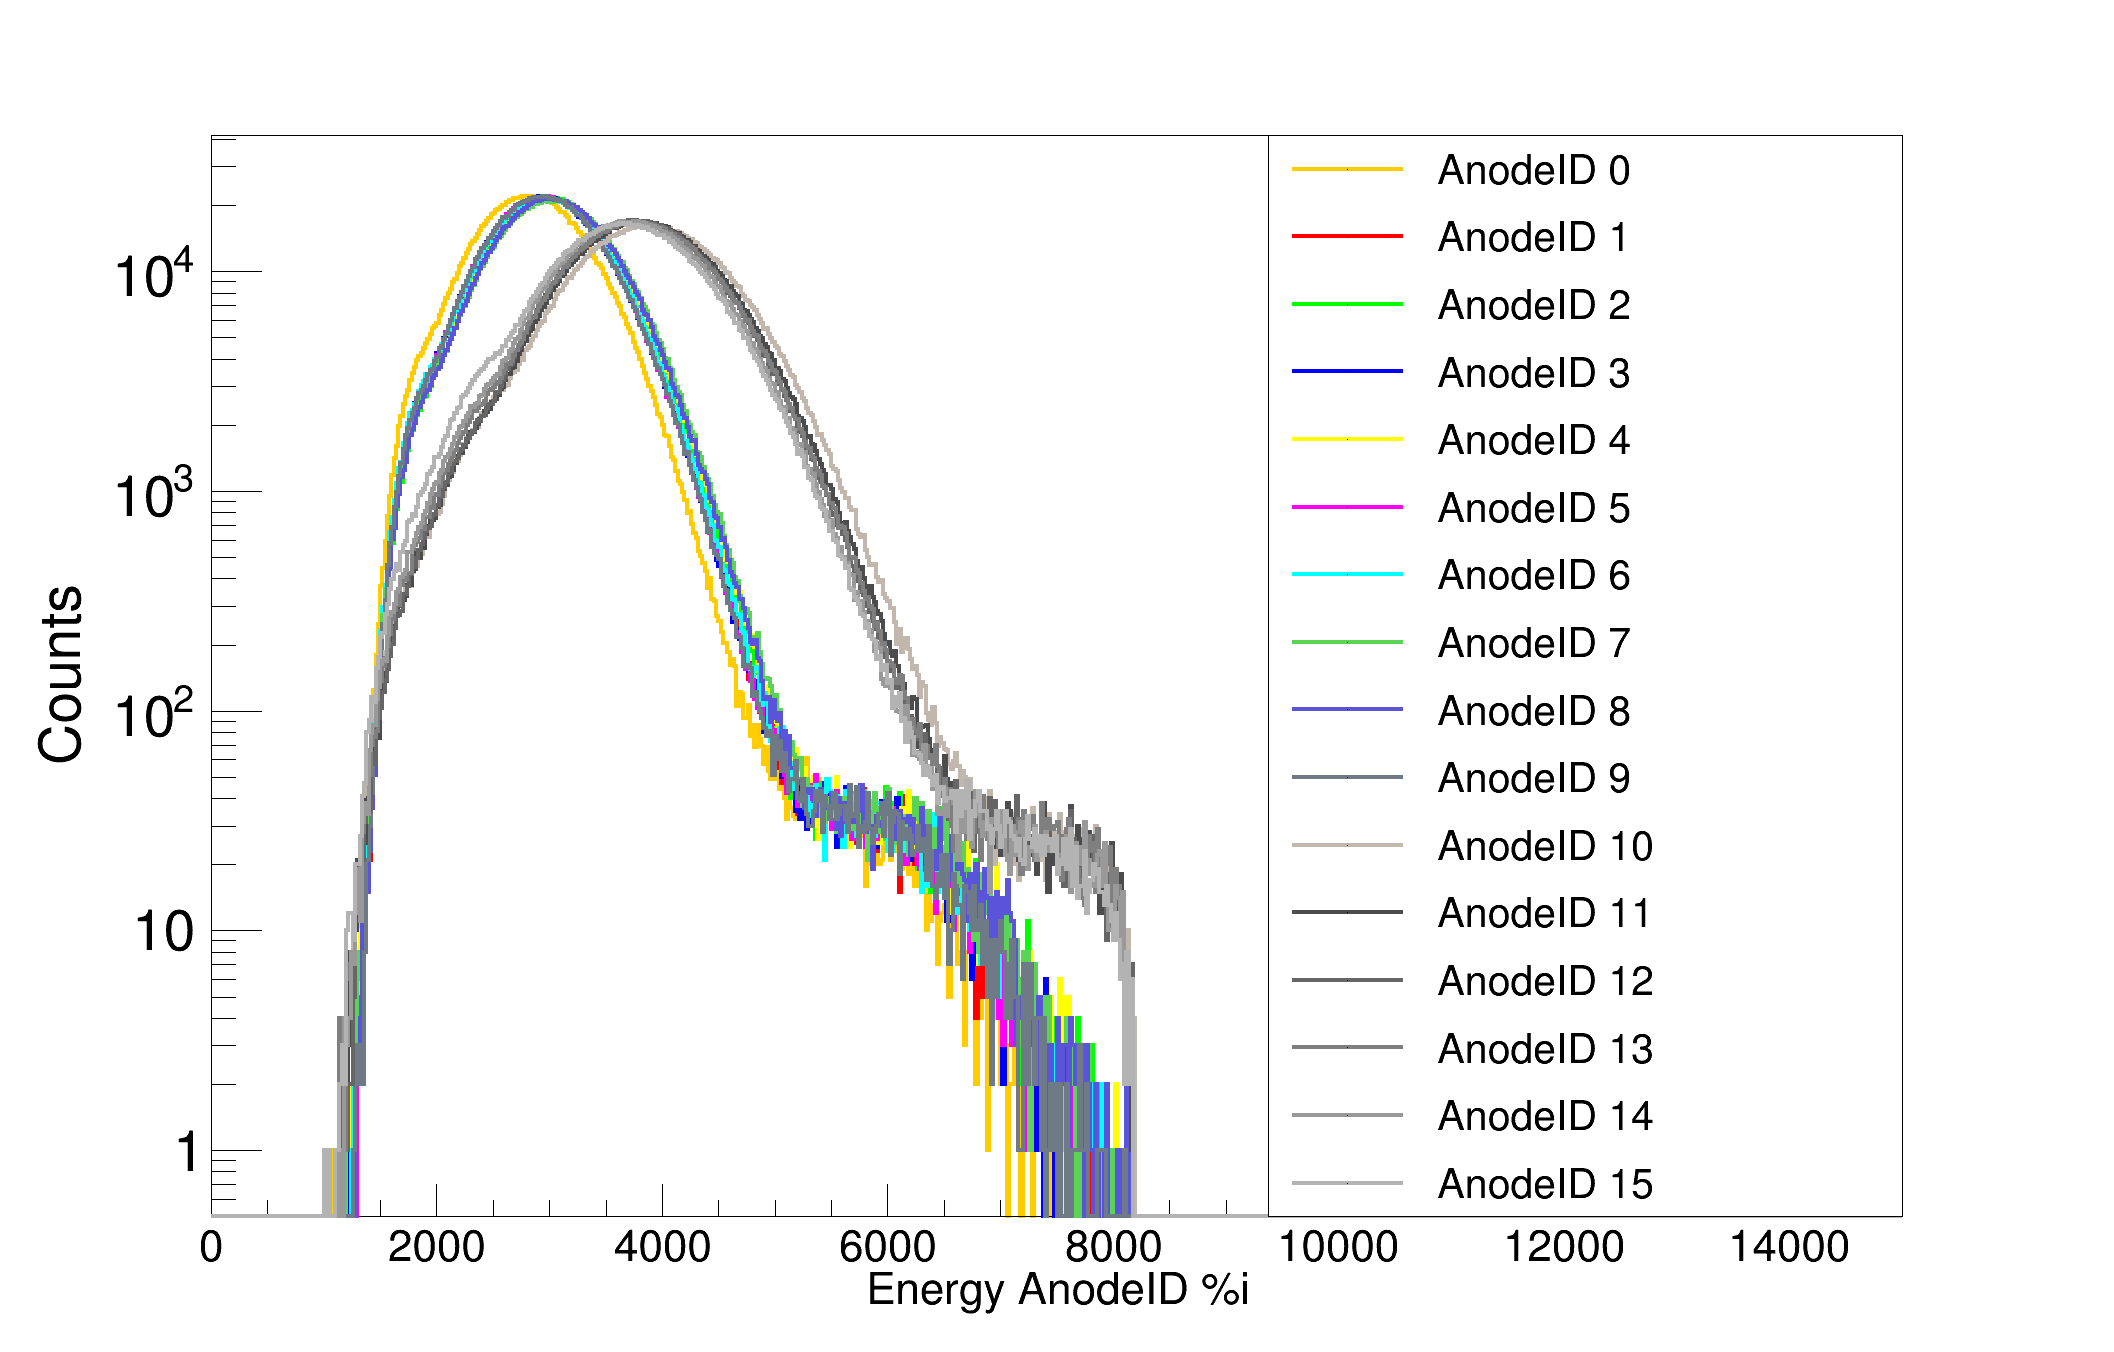
\includegraphics[width=\textwidth]{Figures/twim_mapped_550.png}
         \caption{Uncalibrated raw $\Delta E$ distributions for all 16 anodes for the thick target run, 550 AMeV beam energy.The last six anodes have a slightly different electronics amplification chain.}
         \label{fig:raw_twim}
     \end{subfigure}
     \hfill
     \begin{subfigure}[t]{0.45\textwidth}
         \centering
         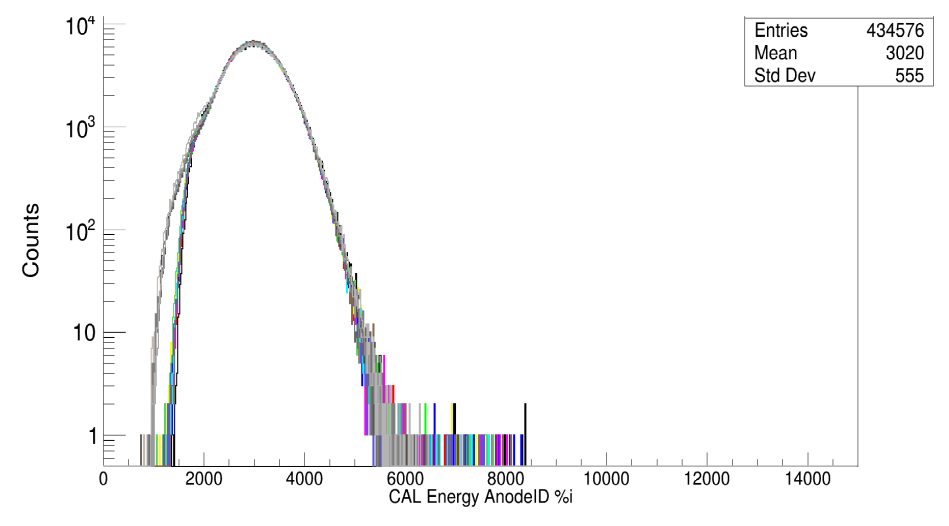
\includegraphics[width=\textwidth]{Figures/twim_mapped_550_no_calib.png}
         \caption{Gaussian fit applied to prominent peak and shifted to same position.}
         \label{fig:cal_twim_one}
     \end{subfigure}
     \hfill
        \caption{Fitting procedure in TWIN.TODO: nicer labeling!}
        \label{fig:calibration}
\end{figure}
\subsubsection{TWIN MUSIC Event Selection}
As previously stated cuts on the downstream detectors are avoided. However, events which have hits in one or several anodes in TWIN MUSIC but no signal in the reference anode are discarted as a whole neither contributing to $N_1$ (incoming selected ions) nor to $N_2$ (unreacted ions). If no reference time from start CFD signal is available it is not possible to measure the drift time in the individual anodes which makes it not possible to distinguish between signal and noise hits for multi-hit anode events in TWIN MUSIC. The number of events affected by this cut is in the region of few tens. This is negligible to the number of incoming ions $N_1$ and should not have any dependence whether the projectile reacted or not.
\begin{table}[h!]
\centering
\begin{subtable}[c]{1.\textwidth}
\centering
\begin{tabular}{|c|c|c|c|c|}
\hline
\makecell{\# incoming \\ projectiles $N_1$}& 400 & 550 & 650 & 800 \\
      & MeV/nucleon & MeV/nucleon & MeV/nucleon & MeV/nucleon \\
\hline
Empty & 574279{\footnotesize(*451*)} & 453729{\footnotesize(*34*)} & 522451{\footnotesize(*44*)} & 395451{\footnotesize(*52*)} \\
\hline
thin & 569503{\footnotesize(*422*)} & 476323{\footnotesize(*33*)} & 538037{\footnotesize(*43*)} & 481459{\footnotesize(*36*)} \\
\hline
medium & 606578{\footnotesize(*431*)} & 451137{\footnotesize(*27*)} & 500688{\footnotesize(*40*)} & 345654{\footnotesize(*46*)} \\
\hline
thick & 655762{\footnotesize(*497*)} & 436457{\footnotesize(*30*)} & 530869{\footnotesize(*29*)} & 479679{\footnotesize(*61*)} \\
\hline
\end{tabular}
\caption{Number of clean selected incoming $^{12}$C ions. In brackets number of rejected events because of missing tref in TWIN MUSIC. TODO: change the bracket notation, looks like error number!!}
\label{tab:incoming_ions}
\end{subtable}
\newline
\begin{subtable}[c]{1.\textwidth}
\centering
\begin{tabular}{|c|c|c|c|c|}
\hline
\makecell{\# survived carbon \\ isotopes $N_2$}& 400 & 550 & 650 & 800 \\
      & MeV/nucleon & MeV/nucleon & MeV/nucleon & MeV/nucleon \\
\hline
Empty & 563382{\footnotesize(1.898\%)} & 444618{\footnotesize(2.008\%)} & 511923{\footnotesize(2.015\%)} & 387513{\footnotesize(2.007\%)} \\
\hline
thin & 538245{\footnotesize(5.489\%)} & 449422{\footnotesize(5.648\%)} & 507557{\footnotesize(5.665\%)} & 454099{\footnotesize(5.683\%)} \\
\hline
medium & 552763{\footnotesize(8.872\%)} & 410376{\footnotesize(9.035\%)} & 455159{\footnotesize(9.093\%)} & 314119{\footnotesize(9.123\%)} \\
\hline
thick & 553935{\footnotesize(15.528\%)} & 368004{\footnotesize(15.684\%)} & 446115{\footnotesize(15.965\%)} & 402696{\footnotesize(16.049\%)} \\
\hline
\end{tabular}
\caption{Number of survived carbon isotopes after the target identified via 2D gaussian fit with borders within 3.5$\sigma$ cut. In brackets the precentage of projectiles with a charge state of Z < 6 after the target.}
\label{tab:survived_ions}
\end{subtable}
\caption{Numbers of incoming projectiles $N_1$ and survived carbon isotopes $N_2$ for all energy and target runs.}
\label{tab:overview_nr_cccs}
\end{table}
\subsubsection{Carbon Identification}\label{subsec:carbon_id}
The identification of carbon isotopes in TWIN is done by reconstructing fragments with charge Z = 6 from 2D plots where coincident mean energy losses $\Delta E$ for different anode combinations are plotted. Since the TWIN MUSIC is multi-hit capable various strategies were developed to deal with multi-hit events, i.e. when having anodes with multiple hits, decide which hit originates from the final state products from the reaction and which from background and noise.\newline
The default strategy is to use the time information of each hit for selection. It has to be remarked that for the S444 experiment the TWIN MUSIC was read out by two independent MDPP modules\cite{MDPP-16}. The signals from the first reference anode and the first eight upstream anodes were sent to module 1, the ones from the last eight downstream anodes and the second reference anode were forwarded to module 2. For the first eight upstream anodes the drift time is calculated by substracting the hit time in each anode by the reference time from the first reference anode and for the last eight downstream anodes accordingly the second reference andode was used.\newline
The time based selection algorithm for multi-hit anodes works as follows:\newline
\begin{enumerate}
\itemsep0em
\item Get the mean drift time for the eight upstream anodes($t_{mean\_up}$) and the eight downstream anodes($t_{mean\_down}$)\footnote{For the case all eight downstream anodes have multiple hits, set $t_{mean\_down} = t_{mean\_up}$ and vice versa}. Anodes with multiple hits do not contribute to this calculation.
\item If there are anodes with muliple hits compare the hit time with the accorging mean drift time ($t_{mean\_up}$ for any of the eight upstream anodes, $t_{mean\_down}$ for any of the eight downstream anodes). Calculate herefore the absolute difference between mean drift time and each hit time:
\begin{equation}
\Delta t = | \bar{t} - {t^i}_{drift}|; \, \text{i = anodeID (1-16) with} \quad \bar{t} = 
\begin{cases}
t_{mean\_up} & \text{for i} \leq 8\\
t_{mean\_down} & \text{for i} \geq 9 \\
\end{cases}
\end{equation}
\item For each anodes with muliple hits select the hit with lowest drift time differnce to the mean drift time.
\end{enumerate}
\begin{figure}[htpb]
    \centering
    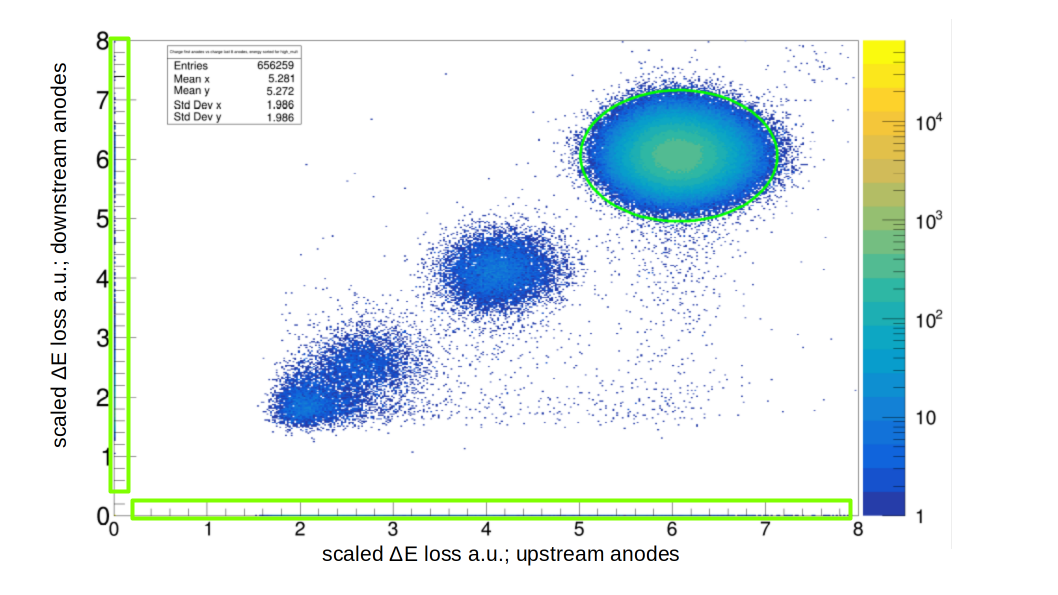
\includegraphics[width=\textwidth,height=8cm,keepaspectratio=true]{Figures/charge_cut_with_out_borders.png}
    \caption{
    Two dimensional gaussian fit with 3.5 $\sigma$ cut  on identified carbon isotopes in TWIN MUSIC. The horizontal and vertical side bars contain events where either the eight upstream anodes or downstream anodes have no hit entry. The cluster at scaled $\Delta E$ loss $\approx$ 4.5 corresponds to boron isotopes (Z=5). The clusters for Z=4 (Be) and Z=3(Li) overlap.
    }
    \label{fig:twin_2d_gaus_cut}
\end{figure}

After having selected the appropriate hit for single and multi-hit anodes the mean value for the pre-calibrated $\Delta E$ loss, see figure \ref{fig:cal_twim_one}, for the eight upstream and accordingly for the eight downstream anodes is determined. Finally, to select the number of survived carbon isotopes the mean $\Delta E$ of the eight upstream anodes versus the mean $\Delta E$ of the eight downstream anodes is plotted. To retrieve the number of survived carbon isotopes following two-dimensional gaussian fit is applied on the 2D plot on the charge Z = 6 blob, see figure \ref{fig:twin_2d_gaus_cut}:
\begin{equation}
f(x) = A e^{-\frac{1}{2}((\frac{x - \bar{x}}{\sigma_{x}})^2 +(\frac{y - \bar{y}}{\sigma_{y}})^2)}
\label{eq:gauss_fit}
\end{equation}
where x is the mean rescaled energy loss of the first upstream andodes and y the according eight downstream anodes. The number of survived carbon isotopes is given by the integral of events within the 2D gaussian fit. Since the anodes were read out by two independent MDPP modules with slightly different thresholds also events along the histogram axes with no hit entry in either the upstream anodes or downstream anodes are analyzed. For those events a one dimensional gaussian cut is applied using the parameters from equation \ref{eq:gauss_fit} (see horizontal and vertical bars in figure \ref{fig:twin_2d_gaus_cut}).\newline
To get the charge changing cross section values equation \ref{eq:corr_cross} has to be applied where both the number of survived  carbon isotopes for target run and empty run are determined via the 2D gaussian fit as in figure \ref{fig:twin_2d_gaus_cut}. The number of target particles, are defined by the target thickness and its density and are listed in section \ref{section:transmission_method}. 
%\begin{equation}
%\begin{split}
%&N_t = \rho \cdot N_A \cdot n \cdot d\\ 
%&\rho = \text{density [$g/cm^3$]} = 1.851 g/cm^3,\text{taken from \cite{ponnath2023precise}}\\
%&N_A = \text{Avogadro constant} =  6.02214076 \cdot 10^{23} mol^{-1}\\
%&n = \text{amount of substance [mol/g]} = 1./12.011 \; mol/g\\
%&d = \text{target thickness[cm]}
%\end{split}
%\end{equation}
%Three carbon targets with different thicknesses are given:
%\begin{enumerate}
%\itemsep0em
%\item thin target: d = 0.5451 cm
%\item medium target: d = 1.0793 cm
%\item thick target: d = 2.1928 cm 
%\end{enumerate}
\begin{figure}[htpb]
    \centering
    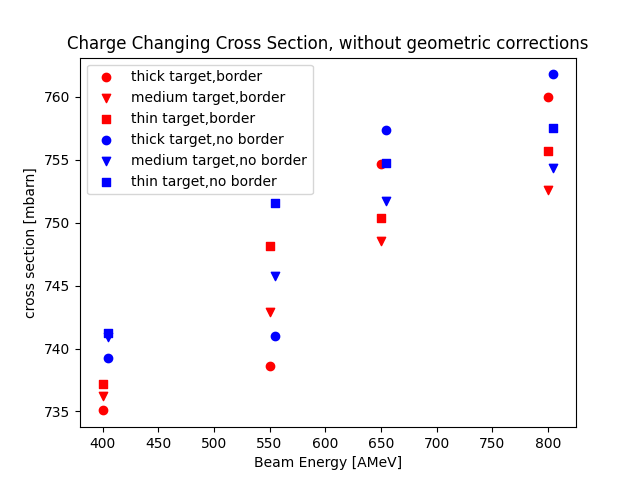
\includegraphics[width=\textwidth,height=8cm,keepaspectratio=true]{Figures/cccs_with_out_border_3_5_sigma.png}
    \caption{
    Charge changing cross section without geometry corrections. The red data points result from considering also events with only hits in the upstream or downstream anodes, the blue data points don't take these events in consideration. 
     }
    \label{fig:cccs_with_out_border_3_5}
\end{figure}
The resulting charge changing cross sections are summarized in figure \ref{fig:cccs_with_out_border_3_5} once with consideration of the vertical/horizontal bars in figure \ref{fig:twin_2d_gaus_cut} and once without. Hits within the 3.5 $\sigma$ gaussian fit are identified as carbon isotopes.
To get the optimal $\sigma$ cut on the two dimensional gaussian fit on the energy losses of the upstream anodes versus downstream anodes the charge changing cross section for all targets and all energies was systematically measured for $\sigma$-cuts in the range of 1 to 5 $\sigma$, see figure \ref{fig:cccs_vs_sigma_cut}. In the region $\thicksim$ 3.5$\sigma$ the variation of the cross section is minimal.
\begin{figure}[htpb]
    \centering
    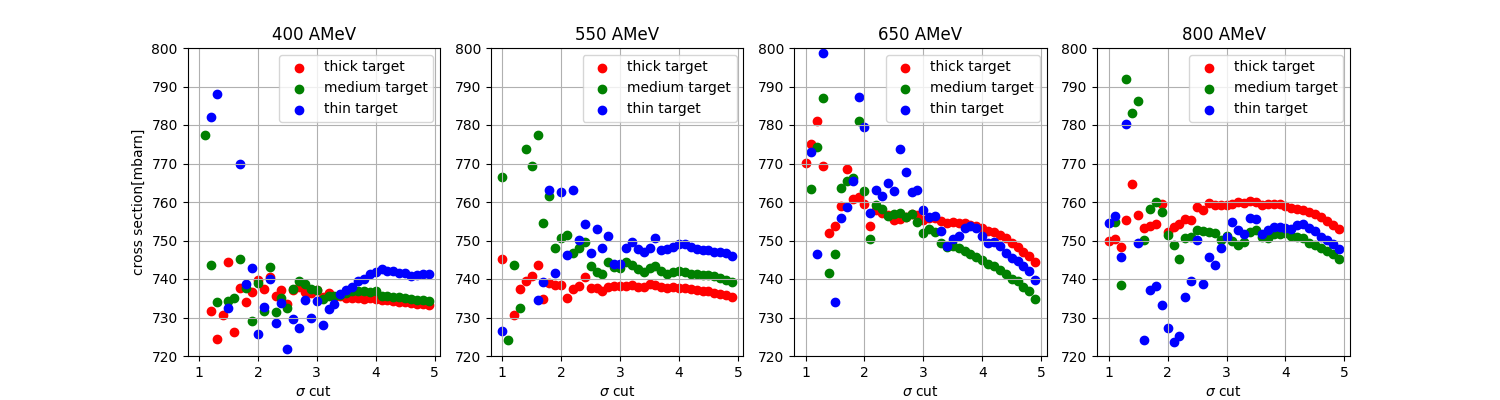
\includegraphics[width=\textwidth,height=8cm,keepaspectratio=true]{Figures/cccs_vs_sigma_cut.png}
    \caption{
    Measured charge changing cross sections according to the $\sigma$ cut applied on the figure \ref{fig:twin_2d_gaus_cut} (with borders) for the different target thicknesses and beam energies.
     }
    \label{fig:cccs_vs_sigma_cut}
\end{figure}
Another method to assert the number survived carbon ions is to apply a diagonal cut on the 2D $\Delta E$ histogram. To set the slope and offset of the diagonal cut line firstly the two dimensional gaussian fit is applied, same as for the previous method. Then the intersection point between the 3.5 $\sigma$ ellipse and the identity line ($\Delta E$ upstream anodes = $\Delta E$ downstream anodes) is found. Through this point, perpendicular to the identity line, the diagonal line is drawn. Everything above the diagonal line is considered as survived carbon ions. Moreover the borders are considered within the 3.5 $\sigma$ cut, see figure \ref{fig:diagonal_cut_twim}. 
\begin{figure}[htpb]
    \centering
    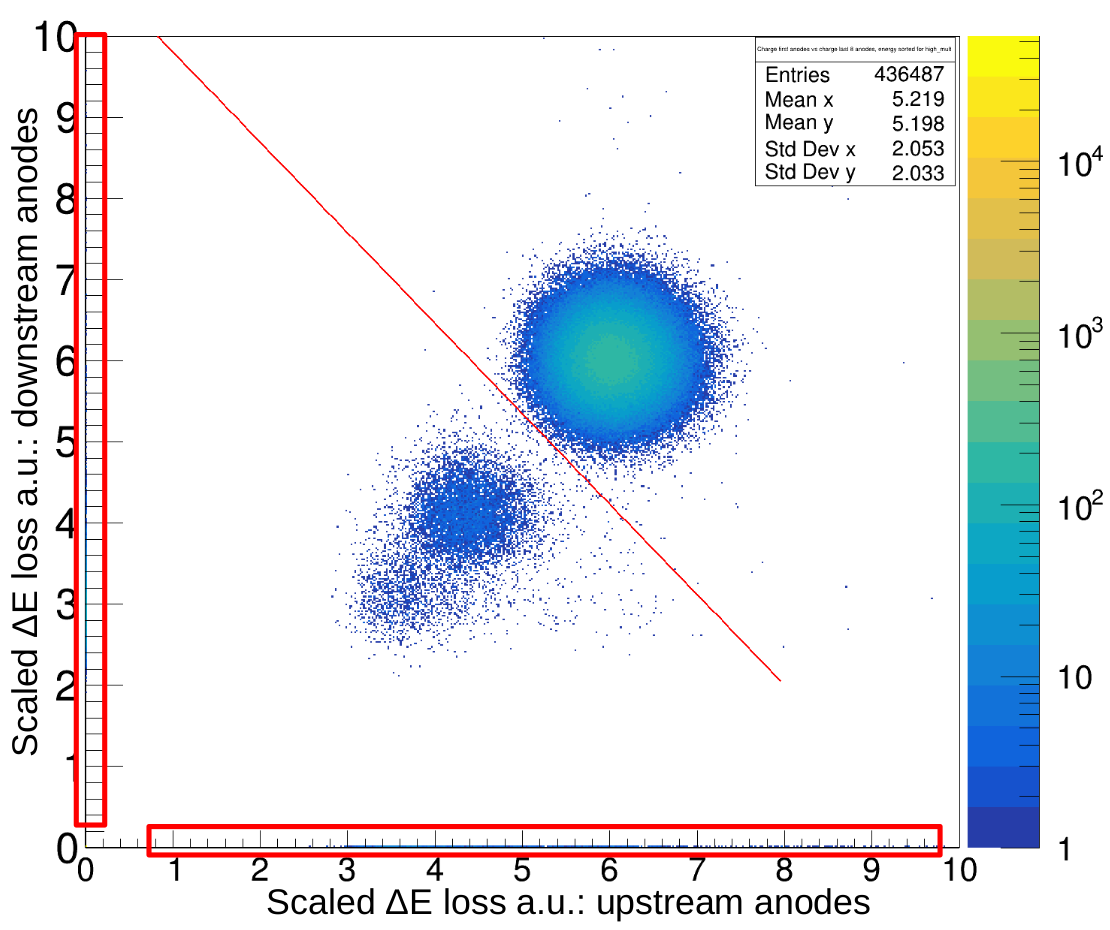
\includegraphics[width=\textwidth,height=8cm,keepaspectratio=true]{Figures/charge_loss_550_thick.png}
    \caption{
    Diagonal cut on identified carbon isotopes along the gaussian 3.5 $\sigma$ cut with borders. All hits above the diagonal line are counted as carbon isotopes. Histogram from thick target run, 550 AMeV beam energy.
     }
    \label{fig:diagonal_cut_twim}
\end{figure}
The effects of the two different methods used for the identification of the carbon isotopes for the charge changing cross section is summarized in figure \ref{fig:cccs_gaus_vs_diag}. The differences in the measured cross sections are within the margin of error herefore both methods are comparable, as expected.
\begin{figure}[htpb]
    \centering
    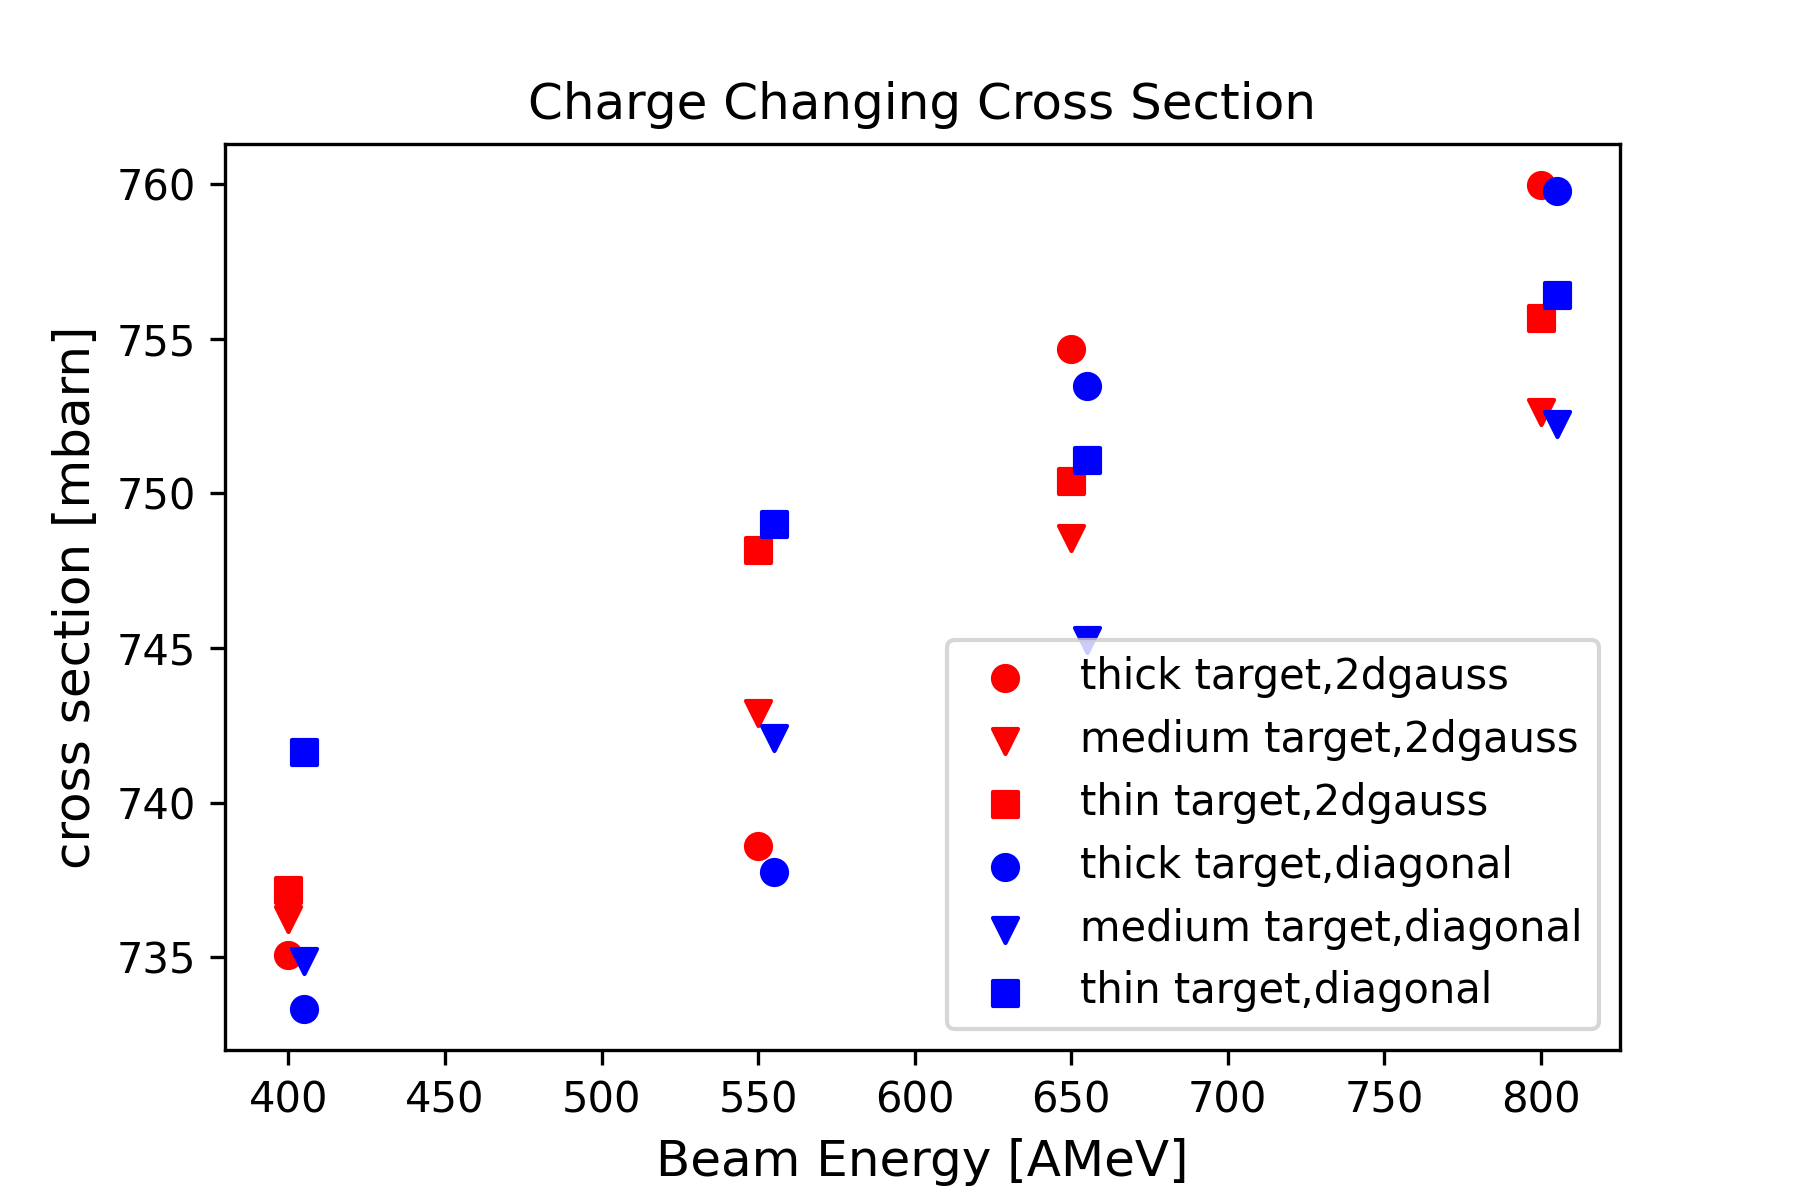
\includegraphics[width=\textwidth,height=8cm,keepaspectratio=true]{Figures/cccs_gauss_diag_comp_3_5_sigma.png}
    \caption{
    Comparison of charge changing cross section measured via 2D gaussian fit cut and diagonal cut. The differnces are within the margin of error.
     }
    \label{fig:cccs_gaus_vs_diag}
\end{figure}
To check wether single anodes or groups of anodes are malfunctioning the charge changing cross section measurement was repeated using only certain anodes for the charge identification:
\begin{enumerate}[label=\alph*)]
\itemsep0em
\item anodes 2-8 versus anodes 9-15 (omitting first and last anode)
\item anodes 1-4 versus anodes 5-8 (upstream anodes)
\item anodes 5-8 versus anodes 9-12 (central anodes)
\item anodes 9-12 versus anodes 13-16 (downstream anodes)
\end{enumerate}
The results from the measurement are summarized in figure \ref{fig:cccs_gaus_diff_sections}. The difference between the default gaussian fit method (with 3.5$\sigma$ cut and considering the borders) considering all 16 anodes and applying the same method but omitting the first and last anode is minimal over all four beam energies. When selecting only 8 out of 16 anodes instead the cross sections are systematically lower when going to high beam energies. The energy loss inside the TWIN MUSIC decreases with higher beam intensities, according to the Bethe-Bloch formula:

%\[
\begin{equation}
-\frac{dE}{dx} = K z^2 \frac{Z}{A} \frac{1}{\beta^2} \left( \frac{1}{2} \ln \frac{2 m_e c^2 \beta^2 \gamma^2 T_{\text{max}}}{I^2} - \beta^2 - \frac{\delta(\beta \gamma)}{2} \right)
\end{equation}
%\]

\text{where:}
\begin{align*}
K &= 4 \pi N_A r_e^2 m_e c^2 \approx 0.307 \, \text{MeV} \, \text{cm}^2 \, \text{g}^{-1}, \\
z &= \text{charge of the incident particle (in elementary charge units)}, \\
Z &= \text{atomic number of the target material}, \\
A &= \text{atomic mass of the target material}, \\
\beta &= \frac{v}{c} = \text{velocity of the particle relative to the speed of light}, \\
\gamma &= \frac{1}{\sqrt{1 - \beta^2}} = \text{Lorentz factor}, \\
T_{\text{max}} &= \text{maximum kinetic energy transferable to an electron in one collision}, \\
I &= \text{mean excitation potential of the target material}, \\
\delta(\beta \gamma) &= \text{density effect correction}.
\end{align*}
The behaviour of dE/dx for small $\beta$- values are dominated by the 1/$\beta^2$ term. The decrease of deposited energy for larger beam energies has as consequence a lower relative resolution in the two dimensional $\Delta E$ loss histogram (see figure \ref{fig:twin_2d_gaus_cut}) reflecting the poissonian distribution properties. In addition reducing the number of readout anodes by a factor two degrades the resolution by a factor $\sqrt{2}$\footnote{It can be assumed a similar $\Delta$ E distribution for all anodes. Hence the central limit theorem can be applied where $\sigma = \frac{\sigma_{anode}}{\sqrt(n)}$ with $n = number of anodes$.}. This has as consequence that the ellipsis with 3.5$\sigma$ cut incorporates a non negligible amount of boron isotopes which are counted as survived carbon isotopes which in turn reduces the measured charge chaning cross section.\newline
\begin{figure}[htpb]
    \centering
    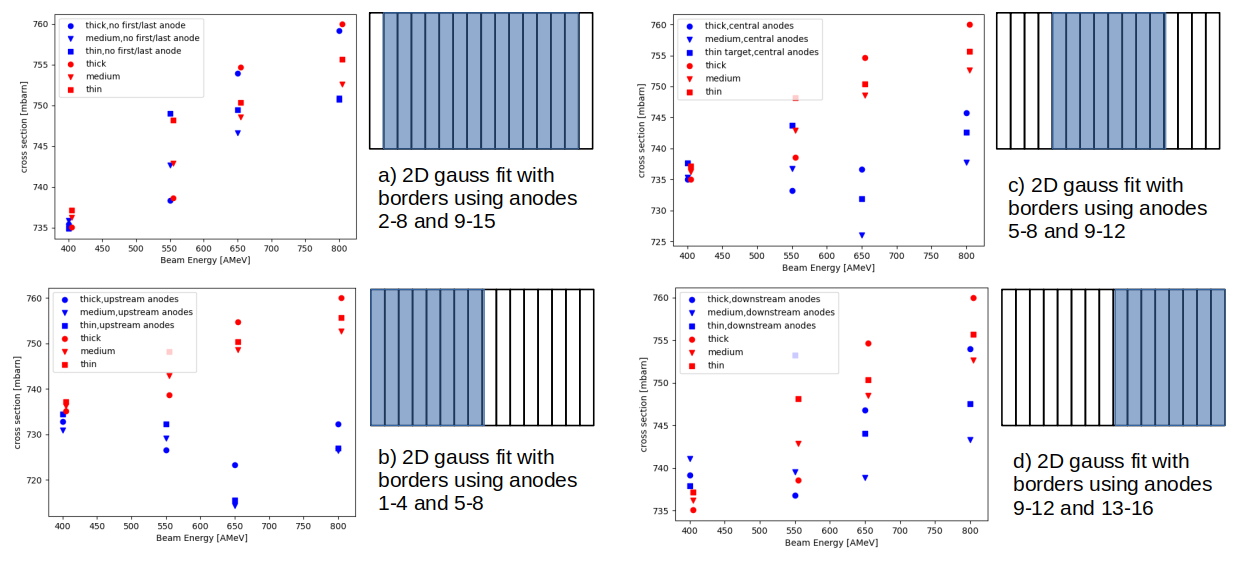
\includegraphics[width=\textwidth,height=8cm,keepaspectratio=true]{Figures/cccs_various_sections_2dgauss_border.png}
    \caption{
   	Measurement of charge changing cross sections using different anode sections to make the two dimensional gaussian fit on the identified carbon isotopes. Red: using all 16 anodes. Blue: the various combinations. 
     }
    \label{fig:cccs_gaus_diff_sections}
\end{figure}
While in the above measurements a time based secelction algorithm for multi-hit anodes was used also an energy based selection was tested. This algorithm selects for multi-hit anodes the hit with the highest energy as physical hit and discarts all others, as they are considered as background/noise. Figure \ref{fig:cccs_gaus_time_vs_energy} compares the time based method versus the energy based method. In both cases a two dimensional gaussian 3.5$\sigma$ cut is applied as in figure \ref{fig:twin_2d_gaus_cut} and the borders are counted as well. The difference in the outcome is negligible. This can be explained since noise or background signal should be both uncorrelated to the event time and at a low energy level and are therefore filtered by both algorithms.
\begin{figure}[htpb]
    \centering
    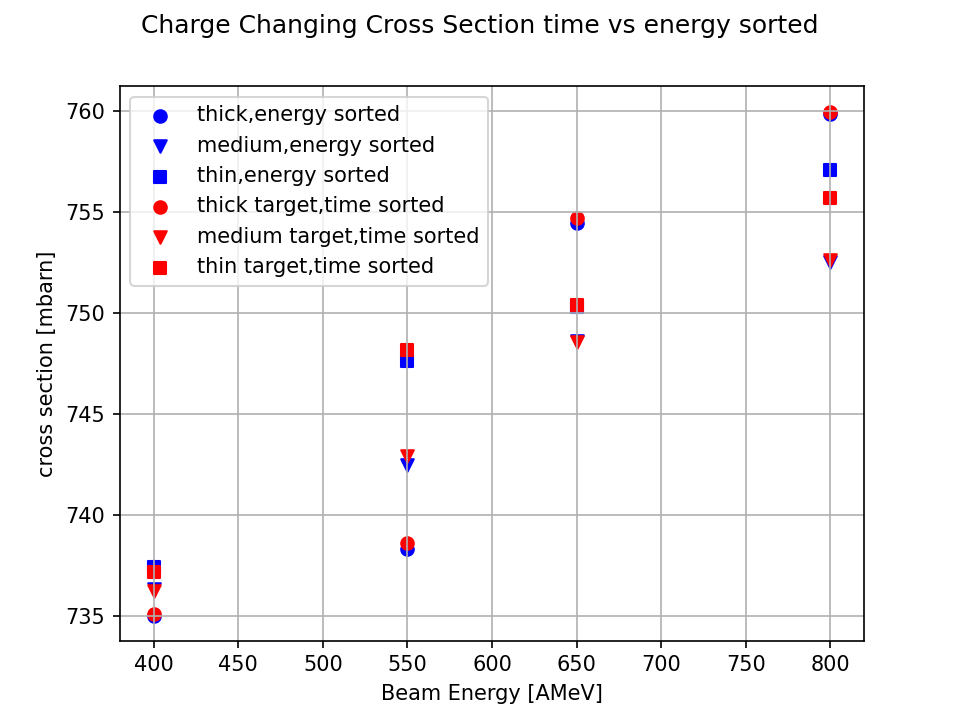
\includegraphics[width=\textwidth,height=8cm,keepaspectratio=true]{Figures/cccs_time_vs_engergy_sorted.png}
    \caption{
    Comparison of charge changing cross section measurements when using time sorting algorithm(red) and energy sorting algorithm(blue) for multi-hit anodes.
     }
    \label{fig:cccs_gaus_time_vs_energy}
\end{figure}
The final charge changing cross section measurements with 2D gaussian fit applying a 3.5 $\sigma$ cut and including the borders of the histogram are summarized in figure \ref{fig:cccs_gaus_with_errors}. At this stage also the statistical errors are incorporated. 
%TODO: Description of statistical gaussian error propagation (refer to L.Ponnath thesis).
\begin{figure}[htpb]
    \centering
    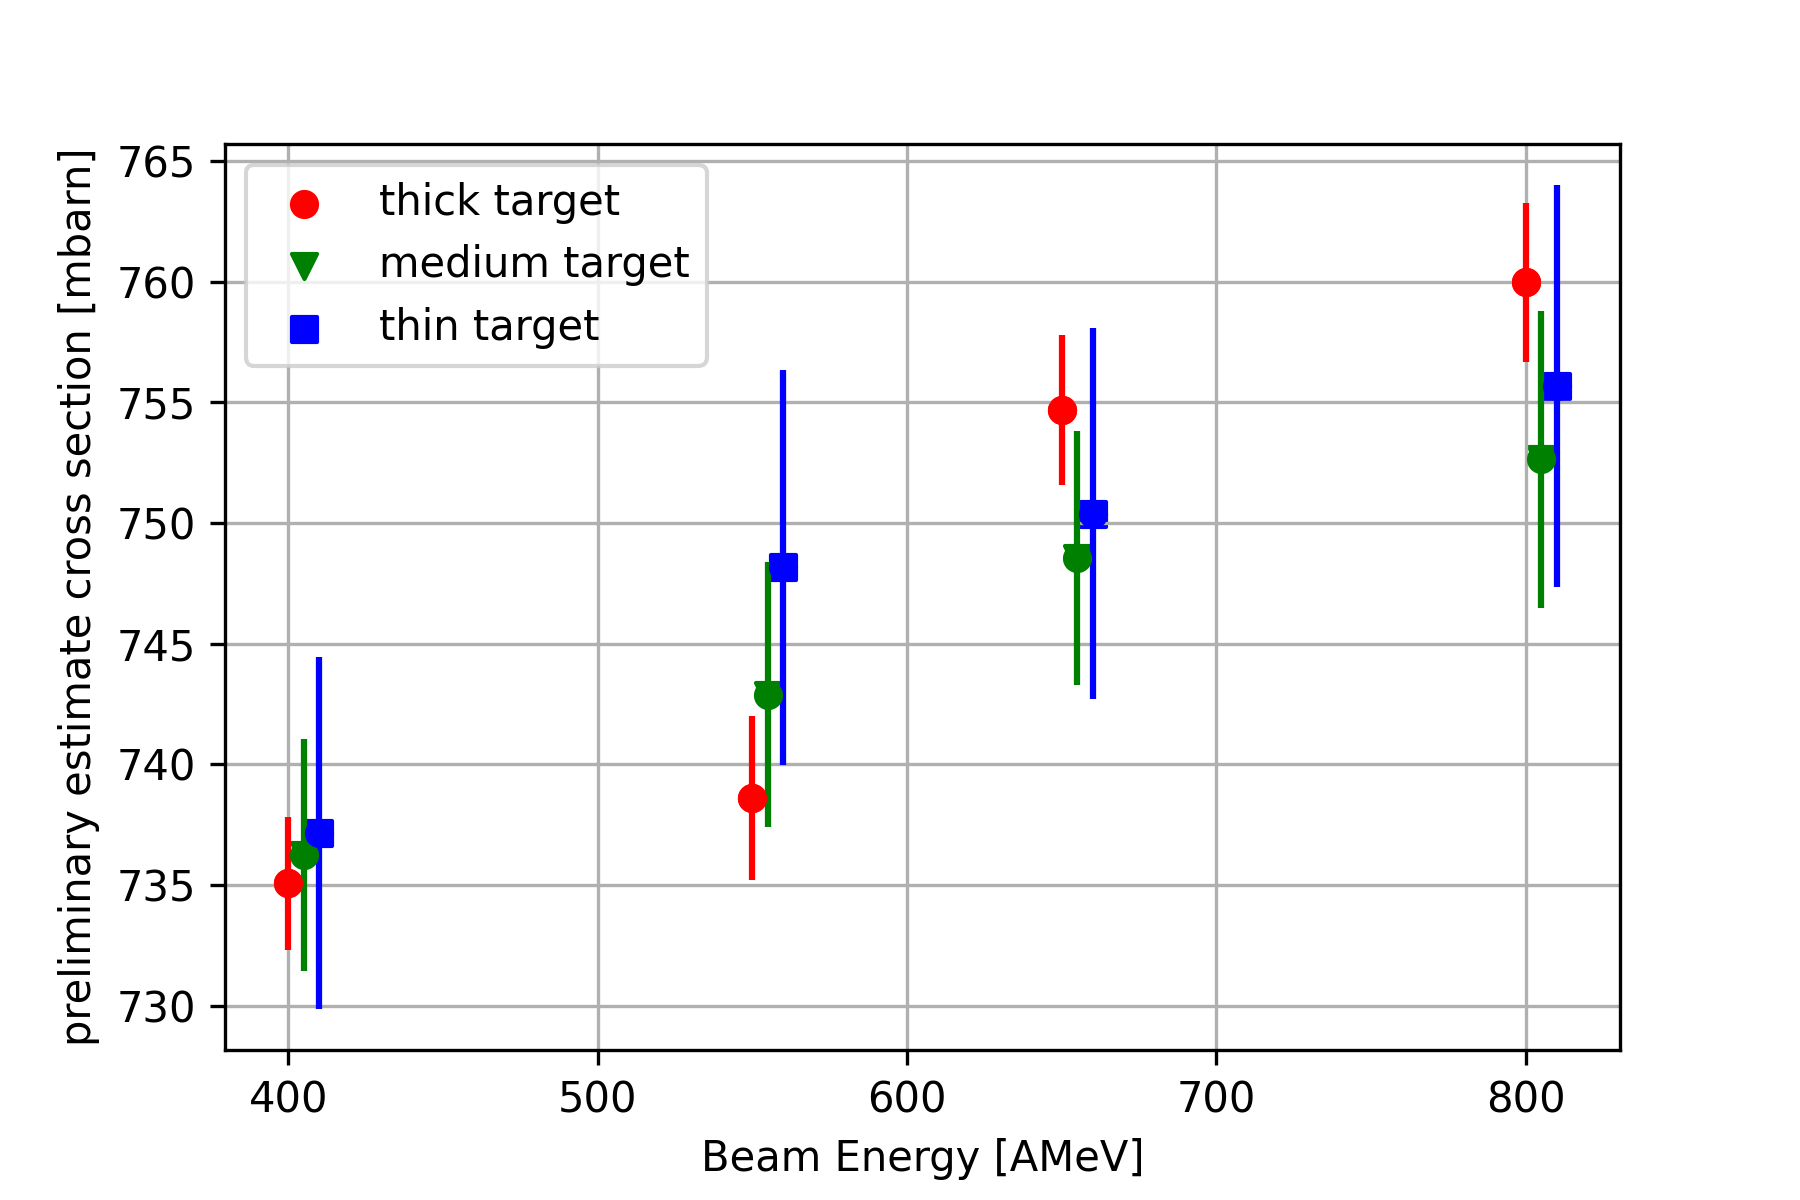
\includegraphics[width=\textwidth,height=8cm,keepaspectratio=true]{Figures/cccs_with_stat_errors.png}
    \caption{
    Measurement of charge changing cross sections using all 16 anodes of the TWIN MUSIC applying the 2D gaussian fit and considering the borders as in figure \ref{fig:twin_2d_gaus_cut}.
     }
    \label{fig:cccs_gaus_with_errors}
\end{figure}

\newpage
%note that thickness calc from Lukas --TODO
%-> deltaE possonian distributed, according to central limit theorem, the sum too DONE
%-> therefore plot Esum of first 8 anodes vs Esum of last 8 anodes DONE
%-> two modules were used for readout DONE
%-> For selecting charge = 6 make gaussian fit on Esum up down DONE
%-> Compare charge = 6 cuts: DONE
%	-->show gaussian 2D cut, for all sigmas (with and whithout borders)
%	-->show gaussian diagonal cut for all sigmas (with and without borders)
%	-->show effect when discarting first/last, first two/last, first three/last and only using last 8 or last 6 anodes with fixed sigma cut
%	
\subsection{Geometric Corrections}\label{sec:geo_corr}
For the S444 experiment only section 1 (right down) of the TWIN MUSIC, which was centered on the beam spot, was operated. As consequence full geometric efficiency could not be assumed. To visualize the restricted geometic efficiency of the TWIN MUSIC the position in x and y (perpendicular plane to the beam direction) on the MWPC1 in front of the ionisation chamber was plotted, once without any conditions on the TWIN MUSIC and once with the condition of having identified a carbon isotope (with the 2D gauss-fit method as described in chapter \ref{subsec:carbon_id}), see figure \ref{fig:mw1_xy}. The large active surface area of 200 x 200 mm$^{2}$ of the MWPC1 affirms that all the carbon fragments are detected\footnote{This statement does not hold for light fragments as protons or deuterons. Their deflection angle exceeds the geometric acceptance of the MWPC1.} whereas the TWIN MUSIC behind it, with an active survace of 55 x 110 mm$^{2}$ (section 1), is not sensitive to the scattered fragments with large deflection angle.\newline
\begin{figure}[htpb]
    \centering
    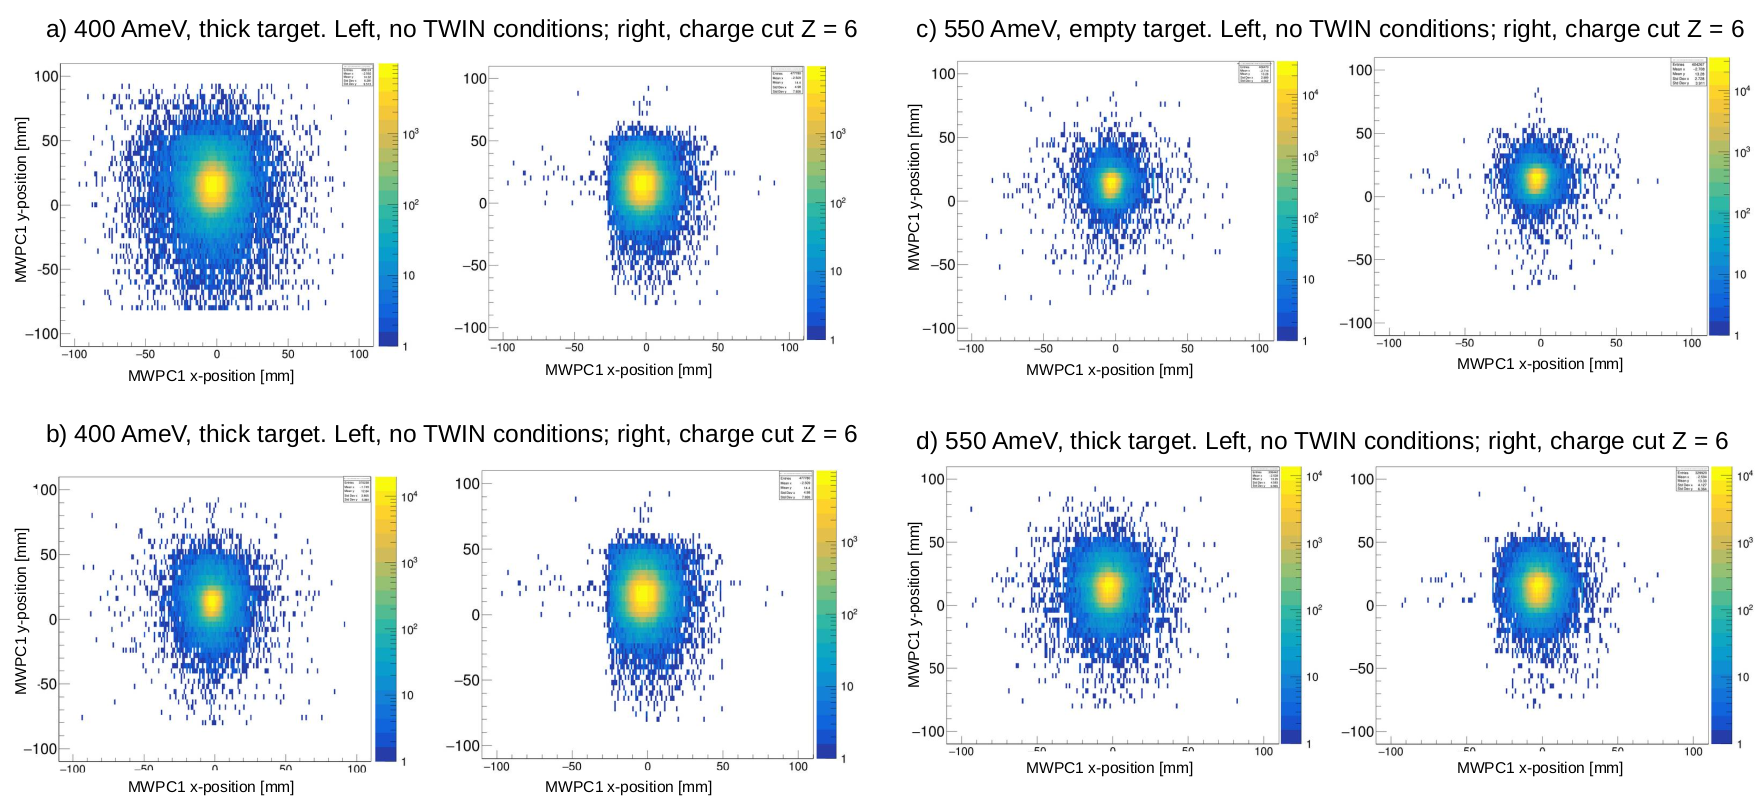
\includegraphics[width=\textwidth,height=8cm,keepaspectratio=true]{Figures/geo_corr_examples.png}
    \caption{
    Distribution in x and y on MWPC1 for different energies with and without target. TODO: subplot b) wrong naming,it's the empty run 400 AMeV. 
     }
    \label{fig:mw1_xy}
\end{figure}

The efficiency loss depends on the target thickness - for thicker targets the geometric distribution of the fragments is broader and therefore the efficiency loss larger - and the beam energies - for larger beam energies the scattering angles decrease due to the boost effects, the efficiency loss gets smaller. This means, that the efficiency loss needs to be compensated runwise. These efficiency effects can be observed in figure \ref{fig:mw1_xy}.\newline
To compensate correctly for the geometric efficiency it has to be considered that for the charge changing cross section measurement only the carbon isotopes after the target are counted in the TWIN MUSIC. Therefore the correction should only be applied to the carbon isotopes (Z = 6) on the x-y distribution on the MWPC1, see figure \ref{fig:mw1_xy}. The geometric efficiency correction is done graphically on the x-y distribution of the MWPC1 for carbon isotopes by following procedure:
\begin{enumerate}
\itemsep0em
\item \textbf{Correction for the x-position distribution:}
%\item TODO: insert x-Distribution in MW1 and the fitted functions
\begin{enumerate}
\item First fit x-distribution with double-gaussian function with five free parameters and common mean value $\mu_x$
\begin{equation}
f(x) = A \cdot exp\left(-\frac{(x-\mu_x)^2}{a^2} \right) + B \cdot exp\left(-\frac{(x-\mu_x)^2}{b^2} \right)
\end{equation}
\item Fit again within range $\mu_x \pm \epsilon_x$.The parameter $\epsilon_x$ is fixed by educated guess, TODO.As $\mu_x$ take the value from the fit in the previous step. A fit for the central region of the x-distribution is obtained,\newline
$f(x)_{central}(A_{central},a_{central},B_{central},b_{central},\mu_{central})$.
\item The obtained fit function $f(x)_{central}$ is then used to compare with the data distribution($f(x)_{data}$) in the border regions [-100,$\mu_{central}-\epsilon_x$] and [$\mu_{central} + \epsilon_x$,100]. Since only the left border region (low x-positions) is affected by the limited geometric acceptance, the right border region can be used for correction:
\begin{equation}
\Delta_{xcorr} = \int_{\mu_{central} + \epsilon_x}^{100} f(x)_{data} - f(x)_{central}\; - \;\int_{-100}^{\mu_{central} - \epsilon_x} f(x)_{data} - f(x)_{central} 
\end{equation}
\end{enumerate}
\item \textbf{Correction for the y-position distribution:}
%\item TODO: insert y-Distribution in MW1 and the fitted functions
\begin{enumerate}
\item First fit y-distribution with double-gaussian function with five free parameters and common mean value $\mu_y$
\begin{equation}
f(y)_{fit} = C \cdot exp\left(-\frac{(y-\mu_y)^2}{c^2} \right) + D \cdot exp\left(-\frac{(y-\mu_y)^2}{d^2} \right)
\end{equation}
\item The obtained fit function $f(y)$ is then used to compare the data distribution($f(y)_{data}$) in the border regions [-100,$\mu_y-\epsilon_y$] and [$\mu_y + \epsilon_y$,100]. The parameter $\epsilon_y$ is fixed by educated guess, TODO. As $\mu_y$ take the value from the fit in the previous step. Same as for the x-correction both border regions are compared. The high border region (high y-positions) affected by the limited geometric acceptance while the low border region (low y-positions) has full geometric acceptance.
\begin{equation}
\Delta_{ycorr} = \int_{-100}^{\mu_{central} - \epsilon_y} f(y)_{data} - f(y)_{fit} \; - \; \int_{\mu_x + \epsilon_y}^{100} f(y)_{data} - f(y)_{fit} 
\end{equation}
\end{enumerate}
\item To correct the number of survived carbon isotopes $N_2 = N_{carbon}$ both corrections in x and y are applied\footnote{Under the assumption that x and y are uncorrelated where the x-y distribution on the MWPC1 is given by $f(x,y) = f(x)\cdot f(y)$.}
\begin{equation}
N_2^{corr} = N_2 +\frac{\Delta_{xcorr}+\Delta_{ycorr}}{N_2}
\end{equation}
\end{enumerate}
\begin{figure}[htpb]
    \centering
    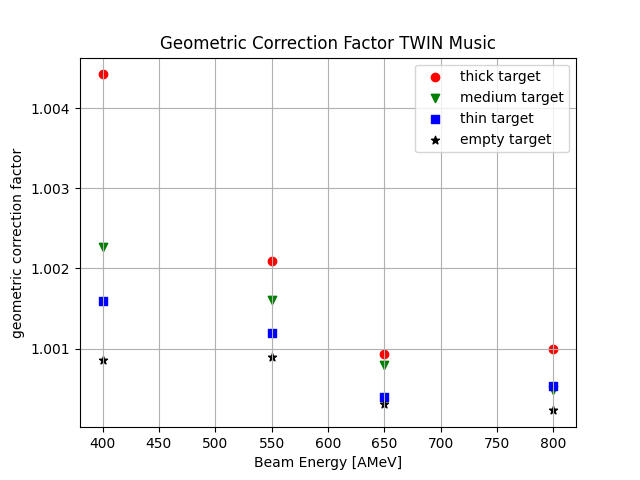
\includegraphics[width=\textwidth,height=8cm,keepaspectratio=true]{Figures/corig_geo_corr_factor.png}
    \caption{
    Geometric correction factors from limited geometric efficiency of TWIN Music. 
     }
    \label{fig:geo_corr_twim}
\end{figure}
Figure \ref{fig:geo_corr_twim} summarizes the geometric correction factors $\epsilon_{geo\textunderscore corr}$ obtained from the graphical reconstruction of missed TWIN Music events as described above. The correction factor is subsequently applied to the charge-changing cross-section, resulting in the final corrected charge-changing cross-section:
\begin{equation}
\sigma_{geo\textunderscore corr} = -\frac{1}{N_t} ln(\frac{N_{1}^E}{N_{2}^E}\frac{N_2}{N_1}\cdot \epsilon_{geo\textunderscore corr}) = -\frac{1}{N_t} \left( ln(\frac{N_{1}^E}{N_{2}^E}\frac{N_2}{N_1}) + ln(\epsilon_{geo\textunderscore corr})\right)
\label{eq:geo_corr_cccs}
\end{equation}
\begin{figure}[htpb]
    \centering
    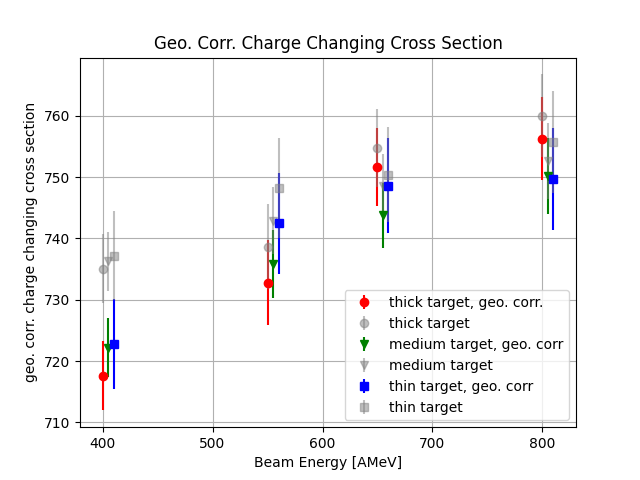
\includegraphics[width=\textwidth,height=8cm,keepaspectratio=true]{Figures/charge_changing_geo_corrected_cross_section.png}
    \caption{
    Charge changing cross section with applied geometry corrections. In gray: charge changing cross section measurements before applying corrections, as in figure \ref{fig:cccs_gaus_diff_sections}. 
     }
    \label{fig:geo_corr_cross_sec}
\end{figure}
Figure \ref{fig:geo_corr_cross_sec} shows the measured charge changing cross section once without considering the the limited geometric acceptance of the TWIM Music and once applying the geometric correction factors as presented in equation \ref{eq:geo_corr_cccs}. As expected significantly affected by the  geometric correction are runs with 400 and 550 AMeV beam energy whereas at beam energies of 650 and 800 AMeV the effect is exceptionally small since at high beam energies  the fragments after the target preceive a strong boost effect in beam direction which constrains the distribution in the x-y-plane.

\subsection{Isotope Correction - Total Interaction Cross Section}
The general formulation for the calculation of cross sections in equation \ref{eq:corr_cross} can be used to determine the cross section for specific channels depending on the definition of $N_2$. In the previous subsection \ref{subsec:cc_cs} where the charge changing cross section was measured, $N_2$ had to be sensitive to the charge of the outgoing fragment. Therefore $N_2$  was  defined as the number of survived carbon isotopes, i.e. $N_2 = N_2^{Z=6}$. For the measurement of the total interaction cross section $N_2$ has to be sensitive to both proton and neutron number of the fragments. $N_2$ is herefore restricted to the number of survived  $^{12}$C isotopes, i.e. $N_2 = N_2^{^{12}C}$. Since $N_2^{^{12}C}$ is a subset of $N_2^{Z=6}$, $N_2^{^{12}C}$ can be determined by identifying and disentangling the number of survived $^{12}$C isotopes from the set of events with carbon isotopes $N_2^{Z=6}$. For that reason the positional correlations on the x-coordinate of MWPC2 (upstream to GLAD) and the MWPC3 (downstream to GLAD) are exploited. The GLAD magnet, which acts as a mass spectrometer, deflects the passing through fragment. Depending on its proton to neutron ratio the fragment is deflected more or less, described by the formula for magnetic rigidity:\newline
\begin{equation}
B\cdot \rho = \frac{\gamma \cdot m \cdot v}{q}
\end{equation}
\text{where:}
\begin{align*}
    B &\quad \text{is the strength of the magnetic field,} \\
    \rho &\quad \text{is the radius of curvature of the particle's trajectory,} \\
    \gamma &\quad \text{is the Lorentz factor,} \\
    v &\quad \text{is the velocity of the particle,} \\
    m &\quad \text{is its mass,} \\
    q &\quad \text{is its charge.}
\end{align*}
Figure \ref{fig:x_mw23_default} shows the x distribution on MWPC2 versus MWPC3 for the thick target run at a beam energy of 400 AMeV. The main diagonal line corresponds to the $^{12}$C isotopes. From all isotopes they have the largest mass to proton ratio (n+p/p) and are therefore less deflected by the magnetic field of GLAD. The less prominent line below corresponds to $^{11}$C isotopes and on the lower edge few events with $^{10}$C are visible. To identify the number of survived $^{12}$C fragments a graphical selection of the $^{12}$C isotopes - the main diagonal line - is applied.\newline
\textbf{Graphical Selection Algorithm:}
\begin{itemize}
\itemsep0em
\item Fit the main diagonal line, which corresponds to the $^{12}$C isotopes, with a linear fit function $f(x_{mw2}) = a \cdot x_{mw2} + b$.
\item To get the most accurate intersection line between $^{12}$C isotopes and all lighter carbon isotopes the linear fit function from the previous step is taken as starting point. Iteratively the offset value $b$ is reduced by $b_i = b_{i-1} -1$. For all iteration steps the ratio $r_{^{12}C(i)}$ of hits below the linear fit function and the total number of hits in the histogram is calculated. 
\item The derivative $\diff{r_{^{12}C}(i)}{b_i}$ is calculated.  
\item Finally the offset $b_i$ with the largest value for $\diff{r_{^{12}C}(i)}{b_i}$ is selected as cutting line between $^{12}$C isotopes and $^{11}$C/$^{10}$C isotopes\footnote{For empty target runs the offset $b$ is manually selected}.
\end{itemize}
The ratio ${r_{^{12}C}}$ is unaffected by detector efficiencies of MWPC2 and MWPC3\footnote{Under the assumption of constant efficiency over $x_{mw2}$ and $x_{mw3}$} and therefore the ratio ${r_{^{12}C}}$ can be applied directly as  isotope correction to calculate the total interaction cross section:
%\begin{equation}
\begin{flalign*}
\sigma_I &= \sigma_{geo\textunderscore corr} + \sigma_{iso} &\\
\text{With the isotope correction cross section $\sigma_{iso}$:} & &\\
\sigma_{iso} &= -\frac{1}{N_t} ln(r_{^{12}C}) & 
\end{flalign*}
%\end{equation}\label{eq:tot_inter_cs}
To calculate the isotope correction cross section six different methods were employed and compared with each other:
\begin{itemize}
\itemsep0em
\item \textbf{MWPC2 and MWPC3 hit-level data:}\newline
For all MWPCs the standard  \textit{cal-to-hit} step  sorts the calibrated hits in the detector according to the calibrated charge deposited in the pads. The final position (in mm) is determined by selecting the hit with the highest charge deposition $Q_{max}$ and its left ($Q_L$) and right neighbour ($Q_R$) pads\footnote{In case no charge deposition in one or both neighbours the charge value is set to 1 respectively.}. These charge and position values are inserted in the "hyperbolic squared secant" function \cite{lau1995optimization} with the following charge distribution function:
\[
Q(x) = \frac{a_1}{\cosh^2\left(\frac{\pi (x - a_2)}{a_3}\right)}
\]
\vspace{-0.5em} % Reduces the space between equations
where \(a_1\) is the amplitude of the distribution $Q_{max}$, \(a_2\) its centroid, and \(a_3\) derives as follows:
\[
a_3 = \frac{\pi \omega}{\cosh^{-1}\left(0.5 \times \left(\sqrt{\frac{Q_{\text{max}}}{Q_L}} + \sqrt{\frac{Q_{\text{max}}}{Q_R}}\right)\right)}
\]
\vspace{-0.5em} % Reduces the space between equations
\(\omega\) being the width of the pads. The centroid of the distribution, which is used as final hit position in the \textit{hit-}data level, can be deduced from:
\vspace{-0.5em} % Reduces the space between equations
\[
a_2 = \frac{a_3}{\pi} \times \tanh^{-1}\left(\frac{\sqrt{\frac{Q_{\text{max}}}{Q_L}} - \sqrt{\frac{Q_{\text{max}}}{Q_R}}}{2 \sinh\left(\frac{\pi \omega}{a_3}\right)}\right)
\]
Figure \ref{fig:hyp_function} shows the "hyperbolic squared secant" function with the inserted values for $Q_{max}$, $Q_R$ and $Q_L$. 
\begin{figure}[htpb]
    \centering
    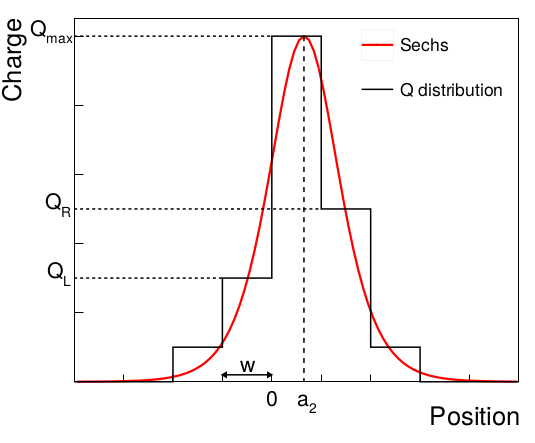
\includegraphics[width=\textwidth,height=8cm,keepaspectratio=true]{Figures/hyperbolic_squared_secant_function.png}
    \caption{
   	 Figure taken from \cite{martin2021fission}, with w being the with of the cathode pads of the MWPC and $a_2$ the final position value of the hit determined by the hyperbolic squared secant function (in red). In black the measured charge deposition distribution in the MWPC. 
     }
    \label{fig:hyp_function}
\end{figure}
The "hyperbolic squared secant" function is used to determine the x hit position as well as the y hit position for all MWPCs. Figure \ref{fig:x_mw23_default} shows the $x_{mw2}$ versus $x_{mw3}$ distribution of carbon isotopes for the 400 AMeV run with the thick target. The two correlated lines corresponding to the $^{12}$C and $^{11}$C isotopes can clearly be distinguished. The vertical line can be interpreted as amount of events where the incoming centered carbon fragment gets scattered by air or the detector material in place between MWPC2 and MWPC3. The horizontal wide spread line has no physical interpretation and can rather be exlained by the \textit{cal-to-hit} step in MWPC2: For events where there is not a spatially constrained hit cluster but sparse hits the hyperbolic squared secant function may pick the wrong $Q_{max}$ and therefore wrongly reconstructs the x position in MWPC2. 
\begin{figure}[htpb]
    \centering
    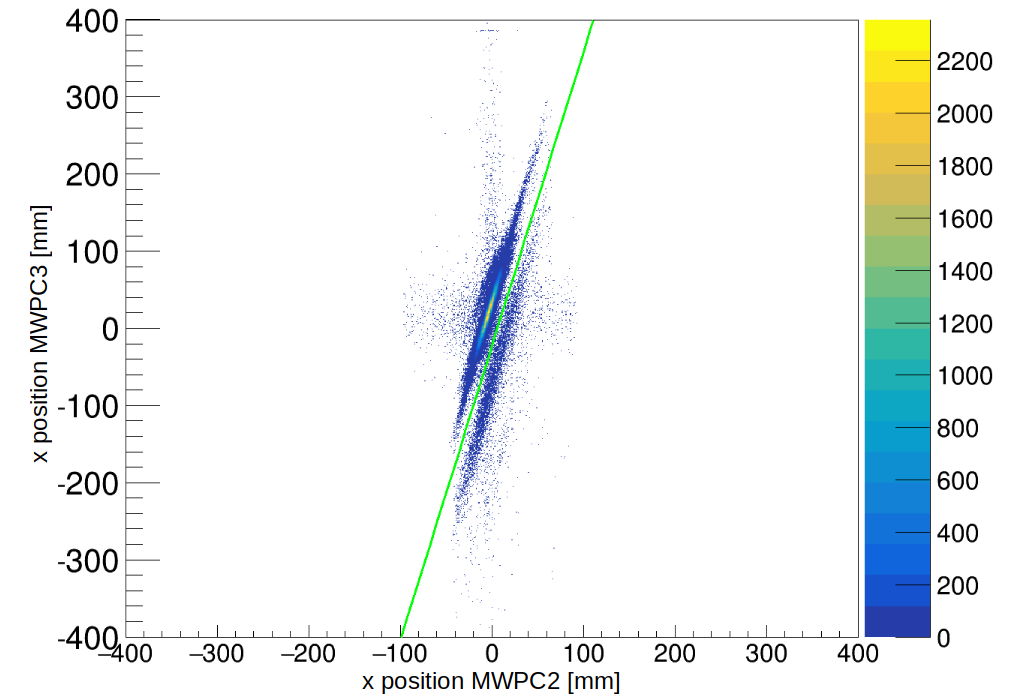
\includegraphics[width=\textwidth,height=8cm,keepaspectratio=true]{Figures/mw23_default.png}
    \caption{
   	 Distribution of x in MWPC2 and MWPC3 for the 400 AMeV run with thick target. The green line corresponds to the intersection line between $^{12}$C and $^{11}$C/$^{10}$C isotopes fixed on the graphical selection algorithm.
     }
    \label{fig:x_mw23_default}
\end{figure}
\item \textbf{MWPC2 and MWPC3 data with own "hit-clustering" level:}\newline 
To overcome the issue with potentially wrong x-position reconstruction in the MWPCs the event selection on MWPC2 and MWPC3 was restricted to events where both MWPC2 and MWPC3 have only one spatially constrained cluster(see figure \ref{fig:own_clustering}) to avoid ambiguities in the position determination. This method strongly retains uncorrelated hits in MWPC2 and MWPC3.\newline
\begin{figure}
\floatbox[{\capbeside\thisfloatsetup{capbesideposition={left,top},capbesidewidth=6cm}}]{figure}[\FBwidth]
{\caption{Resticted event selection for MWPC2 and MWPC3: only events with one single coherent (i.e. without any holes) cluster are accepted.}\label{fig:own_clustering}}
{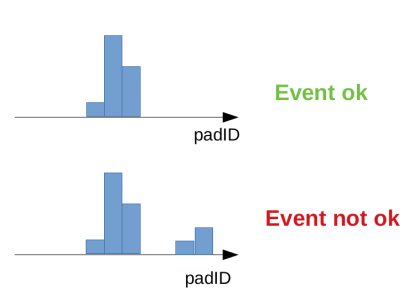
\includegraphics[width=7cm]{Figures/own_clustering_mwpcs.png}}
\end{figure}
Figure \ref{fig:mw23_own_clustering} shows the distribution of x in MWPC2 and MWPC3 using the own hit-clustering reconstruction. This reconstruction method removes the uncorrelated horizontal line which was observed in figure \ref{fig:x_mw23_default}. However the statistics are reduced by $\approx 35\%$\footnote{Number of entries in the 2D plot for default reconstruction method: 533816, for the own hit clustering reconstruction: 346315 for the 400 AMeV run with thick target.}.
\begin{figure}[htpb]
    \centering
    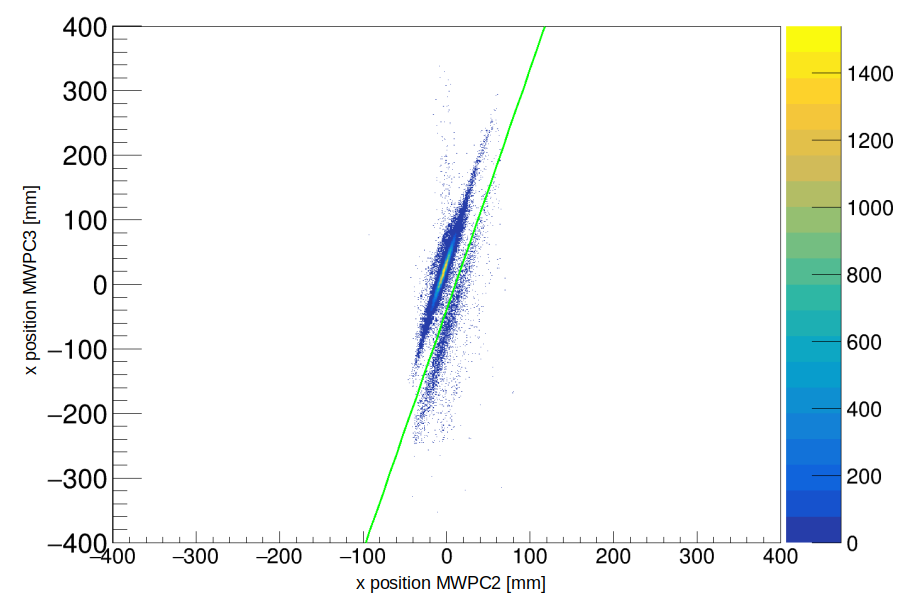
\includegraphics[width=\textwidth,height=8cm,keepaspectratio=true]{Figures/mw23_own_clustering.png}
    \caption{
   	 Distribution of x in MWPC2 and MWPC3 using the own hit clustering reconstruction. Thick target run, beam energy 400 AMeV. The green line corresponds to the intersection line between $^{12}$C and $^{11}$C/$^{10}$C isotopes fixed on the graphical selection algorithm.
     }
    \label{fig:mw23_own_clustering}
\end{figure}

\item \textbf{MWPC1 and MWPC3 hit-level data:}\newline
To get the ratio ${r_{^{12}C}}$ it is necessary to correlate the x positon before and after the GLAD magnet. This task can be completed by MWPC3 with respect to MWPC2 or MWPC1. Since the MWPC1 is upstream to MWPC2 the positional distribution of the carbon fragments narrower which as consequence makes it more difficult to disentangle $^{12}$C and $^{11}$C/$^{10}$C isotopes, see figure \ref{fig:mw13_standard_cluster}. Moreover MWPC1 had two noisy pads which distorts the distribution when using the standard  \textit{cal-to-hit} step to get the position value, see figure \ref{fig:mw13_standard_cluster}.
\begin{figure}[htpb]
    \centering
    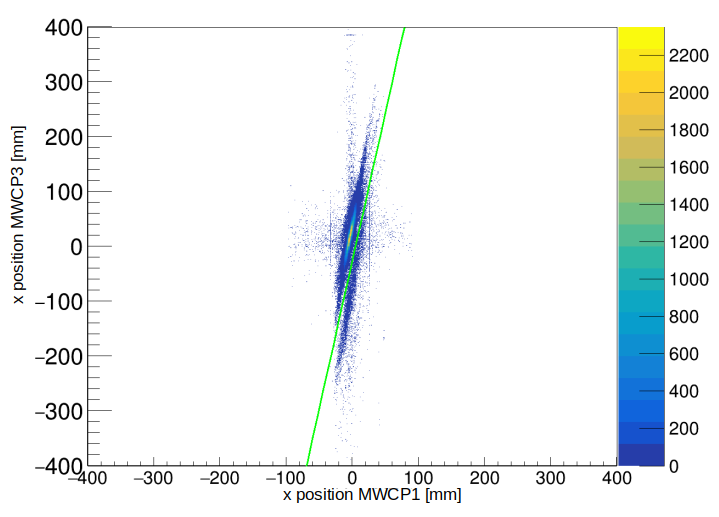
\includegraphics[width=\textwidth,height=8cm,keepaspectratio=true]{Figures/mw13_standard_cluster.png}
    \caption{
   	 Distribution of x in MWPC1 and MWPC3. Thick target run, beam energy 400 AMeV. The two vertical lines stem from two noisy pads in MWPC1. 
     }
    \label{fig:mw13_standard_cluster}
\end{figure}
\item \textbf{MWPC1 and MWPC3 data with own "hit-clustering" level:}\newline
Again, to overcome the issue with potentially wrong x-position reconstruction in the MWPCs the own hit clustering reconstruction method, as described above, was applied to MWPC1 and MWPC3 resulting in the 2D plot \ref{fig:mw13_own_cluster}.
\begin{figure}[htpb]
    \centering
    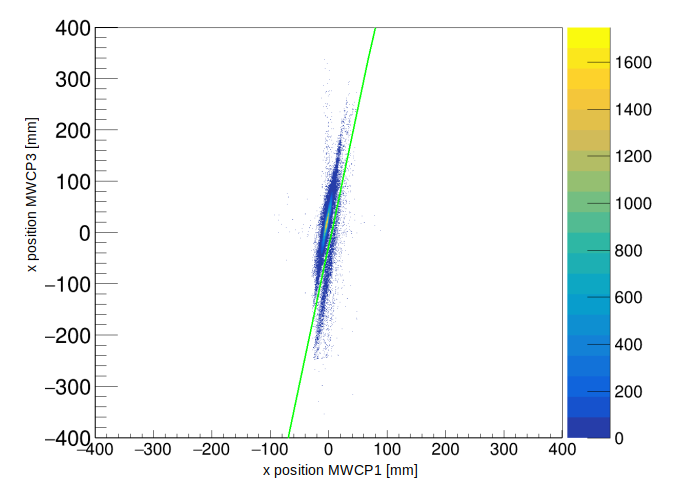
\includegraphics[width=\textwidth,height=8cm,keepaspectratio=true]{Figures/mw13_own_cluster.png}
    \caption{
   	 Distribution of x in MWPC1 and MWPC3 using the own hit clustering reconstruction. Thick target run, beam energy 400 AMeV. 
     }
    \label{fig:mw13_own_cluster}
\end{figure}

\item \textbf{MWPC2 and MWPC3 with own clustering, quadrant selection in MWPC2:}\footnote{I did the quadrant selection also in MWPC2, outcome really similar, TODO: add to appendix...}\newline
The limited geometric acceptance of TWIN MUSIC, described in section \ref{sec:geo_corr}, affects the isotope correction too. The x distribution on the MWPC1/2/3 is cut off on the lower end and the y distribution on the higher end, see figure \ref{fig:mw1_xy}. The $^{11}$C/$^{10}$C isotopes are expected to have a broader x and y distribution. Missing the lower and higher edges in the x and y distribution respectively distorts the ${r_{^{12}C}}$ ratio towards higher values. This results in a lower cross section contribution of the isotope correction, especially for the low energy runs. To correct for this the x-y distribution in MWPC1 was split into four quadrants, see figure \ref{fig:mw1_xy_quadrants}. The intersection lines were derived by the mean of the gaussian fit of the x and y distribution. The cross section contribution of the isotope correction was measured for all four quadrants.
\begin{figure}[htpb]
    \centering
    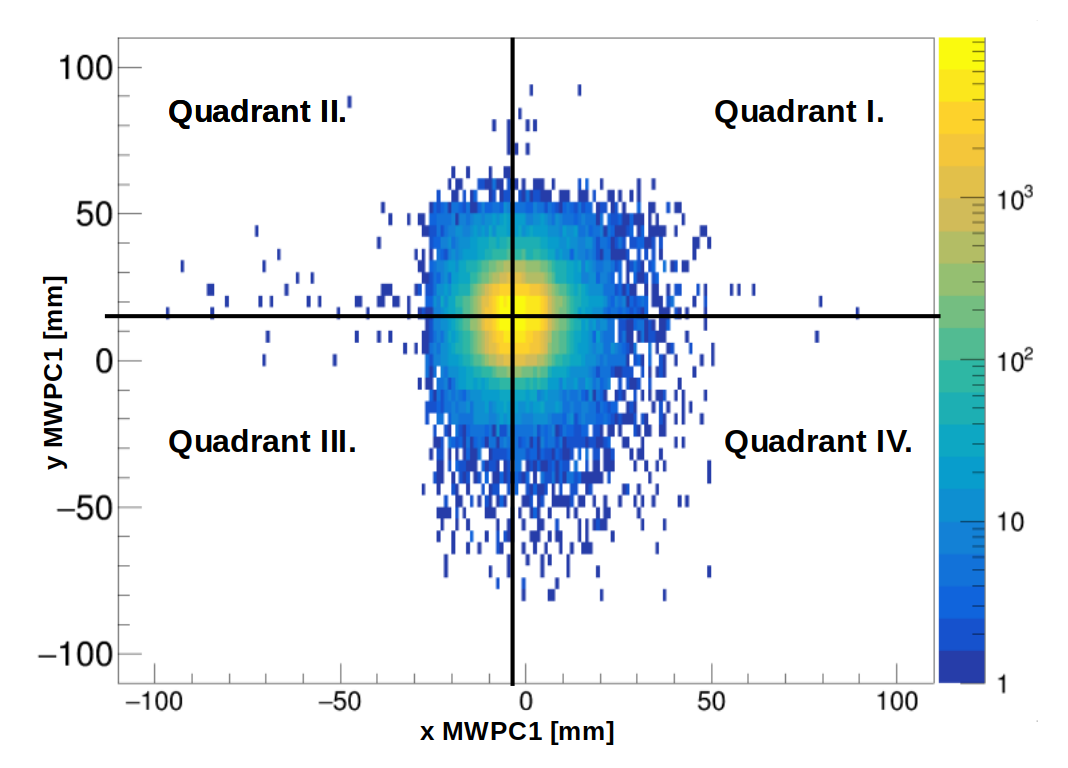
\includegraphics[width=\textwidth,height=8cm,keepaspectratio=true]{Figures/quadrants_mw1_xy_400_thick.png}
    \caption{
   	 Distribution of x and y in MWPC1 split up in four quadrants.Thick target run, beam energy 400 AMeV. 
     }
    \label{fig:mw1_xy_quadrants}
\end{figure}
\end{itemize}
\newpage

\subsubsection{Results for Isotope Correction Methods}
\begin{itemize}
\item \textbf{MWPC2 and MWPC3 hit-level data:}\newline
\begin{figure}[h!]
    \centering
    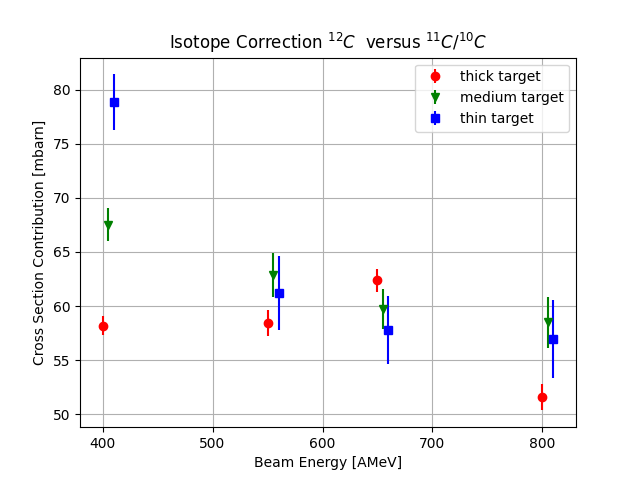
\includegraphics[width=\textwidth,height=8cm,keepaspectratio=true]{Figures/iso_corr_cs_mw23_hit.png}
    \caption{
	Isotope correction contribution to the total interaction cross section using standard hit level data in MWPC2 and MWPC3.
     }
    \label{fig:iso_corr_mw23_default}
\end{figure}

\item \textbf{MWPC2 and MWPC3 data with own "hit-clustering" level:}\newline 
\begin{figure}[h!]
    \centering
    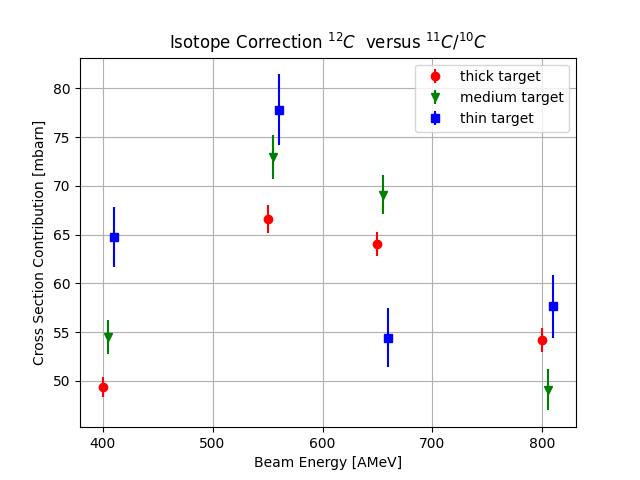
\includegraphics[width=\textwidth,height=8cm,keepaspectratio=true]{Figures/iso_corr_cs_mw23_own_cluster.png}
    \caption{
	Isotope correction contribution to the total interaction cross section using own  hit clustering in MWPC2 and MWPC3.
     }
    \label{fig:iso_corr_mw23_own_cluster}
\end{figure}

\item \textbf{MWPC1 and MWPC3 hit-level data:}\newline
\begin{figure}[h!]
    \centering
    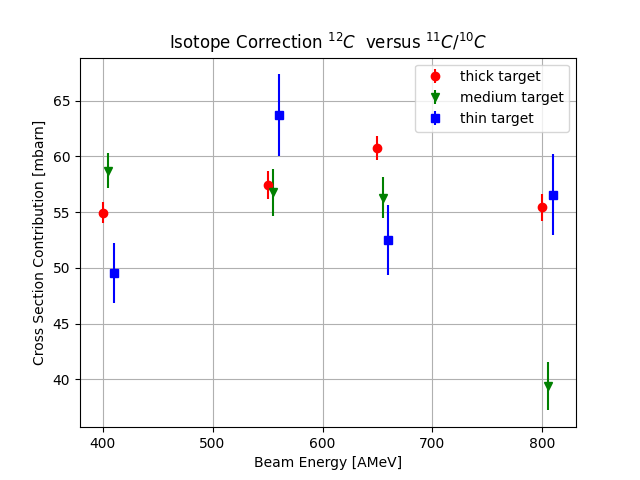
\includegraphics[width=\textwidth,height=8cm,keepaspectratio=true]{Figures/iso_corr_cs_mw13_hit.png}
    \caption{
	Isotope correction contribution to the total interaction cross section using standard hit leved data  in MWPC1 and MWPC3.
     }
    \label{fig:iso_corr_mw13_default}
\end{figure}

\item \textbf{MWPC1 and MWPC3 data with own "hit-clustering" level:}\newline
\begin{figure}[h!]
    \centering
    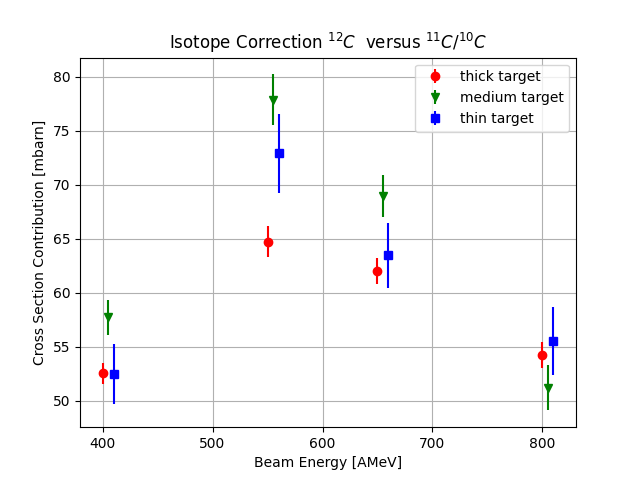
\includegraphics[width=\textwidth,height=8cm,keepaspectratio=true]{Figures/iso_corr_cs_mw13_own_cluster.png}
    \caption{
	Isotope correction contribution to the total interaction cross section using own  hit clustering in MWPC1 and MWPC3.
     }
    \label{fig:iso_corr_mw13_own_cluster}
\end{figure}

\item \textbf{MWPC2 and MWPC3 with own clustering, quadrant selection in MWPC1:}\newline
\begin{figure}[h!]
    \centering
    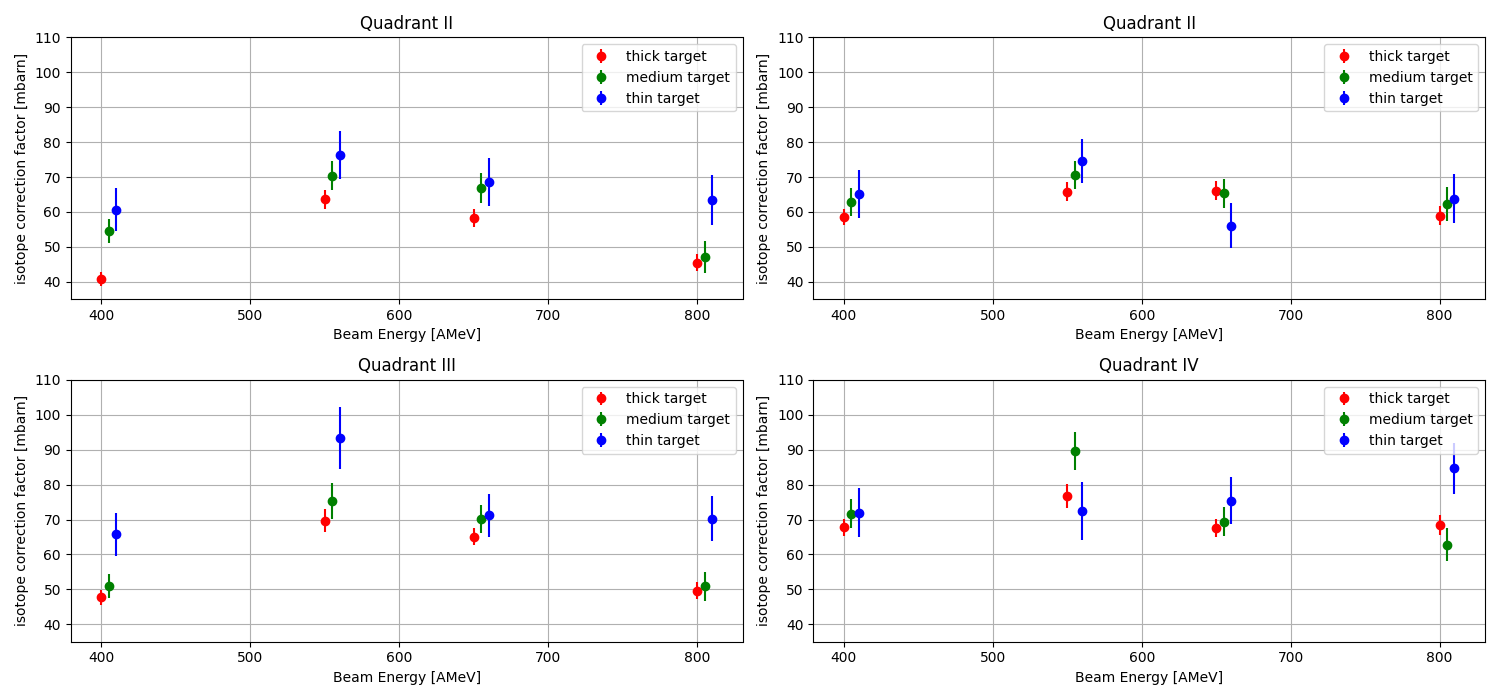
\includegraphics[width=\textwidth,height=8cm,keepaspectratio=true]{Figures/iso_corr_cs_mw23_own_cluster_all_quadrants.png}
    \caption{
	Isotope correction contribution to the total interaction cross section using own  hit clustering in MWPC2 and MWPC3. Comparison for different quadrant selection in MWPC1. Quadrant four is the preferred one as it is not affected by limited geometric acceptance of TWIN MUSIC.
     }
    \label{fig:iso_corr_quadrants_own_cluster}
\end{figure}

\end{itemize}

\newpage
\subsection{Statistical and Systematic Error Analysis}
All three measurements presented in this section, the charge changing cross section, the isotopic cross section correction cross section and the total interaction cross section, rely on the transmission method and the error analysis of those measurements are treated the same accordingly. The generic formula for all three measurements was presented in section \ref{section:transmission_method}, equation \ref{eq:cross_sec}.\newline
Since all quantities in equation \ref{eq:cross_sec} are mutually independent, the gaussian error propagation for statistical and systematical uncetainties is given by:
\begin{equation}
\Delta_{stat./syst.}  = \sqrt{\sum_{i=1}^n \left( \frac{\partial f}{\partial x_i} \cdot \Delta_{x_i} \right)^2 }\
%fi(x_1,x_2,..,x_n): \textrm{the error prone cross section function}\ 
%x_i: \textrm{the independent variables (N_1,N_2,N_t; see equation \ref{eq:cross_sec})}\
%\Delta_{x_i}: \textrm{uncertainties associated to indepenent variable x_i}
\end{equation}
\text{with:}
\begin{align*}
	f(x_1,x_2,..,x_n) &\quad \text{the error prone cross section function,} \\
	x_i  &\quad \text{the independent variables ($N_1$,$N_2$,$N_t$; see equation \ref{eq:cross_sec}),} \\
	\Delta_{x_i} &\quad \text{stat./syst. uncertainties associated to indepenent variable $x_i$}
\end{align*}


\subsubsection{Statistical Uncertainties}


\subsubsection{Statistical Uncertainties}


\subsection{(Preliminary) Results Total Interaction Cross Section}
\begin{figure}[h!]
    \centering
    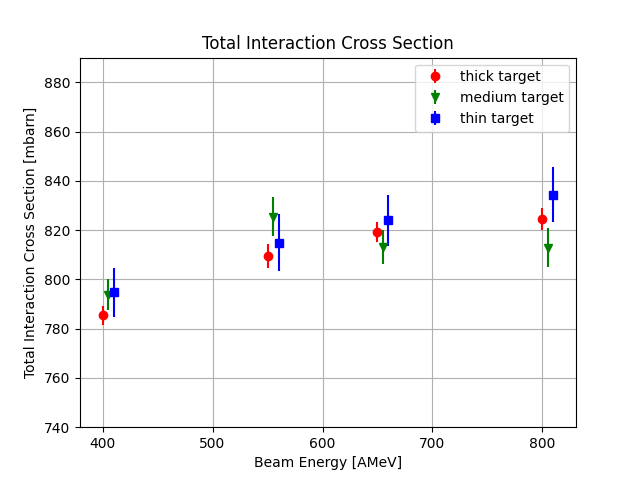
\includegraphics[width=\textwidth,height=8cm,keepaspectratio=true]{Figures/tot_interaction_cs_geo_corr.png}
    \caption{
	Total interaction cross section using the quadrant IV. selection in MWPC1 x-y plot (see figure \ref{fig:mw1_xy_quadrants}) for the isotope correction and applying the geometric correction on the charge changing cross section.}
    \label{fig:tot_interaction_cs}
\end{figure}
\subsection{Quasi-Free Scattering $^{12}$C(p,2p)$^{11}$B}
this is  a reference to \ref{appendix_first}****test
***bottomline: is this really just a subsection?*****
Notes:\newline
\begin{itemize}
\item chapter introduction, first commissioning of p2p reactions at R3B,since first time CALIFA in Final frame and 35\% filled in iPhos
\item what do I have about calibration?
\item channel identification -> Fragment Reconstruction
\item Proton characteristics in Califa
\item inner mom reconstruction, many features here to presen
\item Gamma Spectrum reconstruction / doppler correction (maybe I can use here my own clustering ML stuff?)
\item appendum: separation energy reconstruction? aob? 
\end{itemize}



\subsection{reaction cross section Analysis}


\section{Qualitative Analysis - Quasi-Free Scattering $^{12}$C(p,2p)$^{11}$B}
Until the S444 experiment in 2020 CALIFA consisted out of a prototype frame filled with up to 64 CsI(Tl) crystals. The geometric coverage was therefore limited. For the S444 experiment CALIFA got its final frame and was fully filled in the forward barrel and 35\%filled in the iPhos region, CEPA was not installed yet. With these improvements it was possible to commission QFS-experiments with CALIFA at R$^3$B. In the follow up experiment S467, also in 2020, the first experimental run to study single-particle structures of neutron-rich Ca isotopes via QFS reactions was carried out.\newline
Even though great improvements in the detector development  were achieved the correction factors to correct for geometric acceptance would be much too high ( $\approx$ 10) for precise cross section measurements for QFS-reactions since the correction factors would in turn rely on a a simplified reaction model. A precise analysis of the acceptance correction factor and the development of a more sophisticated and data driven reaction model is out of the scope of this work. Therefore this analysis focusses on the methods of QFS-reaction identification and the extraction of the key informations dicussed in section \ref{sec:qfs_theo}. TODO: add more stuff here...\newline
\subsection{Setup-Calibration}
For setup description refer to section \ref{sec:analysis_cross_sec}. For all detectors except the SOFIA (Study On FIssion with Aladin) Time of Flight Wall the calibration parameters investigated by the respective detector-expert group were adopted. Herefore we will subsequently only describe the Time of Flight Wall calibration in this subsection.
\subsubsection{Flight-Path Reconstruction}\label{subsec:flightpath_reco}
The procedure to calibrate the Time of Flight (ToF) Wall involves beforehand a precise flight-path reconstruction of the projectile from the entrance of Cave C downstream to the ToF Wall. Since only one tracking detector downstream to GLAD was in operation for the S444 experiment no angle of the deflected fragment/beam $\theta_{out}$ could be directly extracted. Herefore an advanced tracking algorithm was developed, motivated from ref. \cite{bertini2013study} (section 3.4). 
\begin{itemize}
\item The first step is to measure the scattering angle after target, $\theta_{in}$, and draw an extended line from the target position through the effective magnetic field of GLAD.  
\item Draw a trajectory line from the hit position in MWPC3 to the intersection point C (see figure \ref{fig:sub1_reco_path}) of the "kick-plane-line" and the reconstructed and extended track line upstream to GLAD.
\item Now sweep along the reconstructed track line upstream to GLAD. For each step a value for $\theta_{out}$ and $d1-d2$ is gathered, see figure \ref{fig:sub2_reco_path}.
\item As in figure \ref{fig:sub2_reco_path} shown, fit the data-points from previous step with a linear fit function and find the corresponding $\theta_{out}$ value where the fit line intersects with the abscissa. This corresponds to the case where $d1 = d2$. This is the approximated "kickpoint" in GLAD. 
\item Previous steps need to be executed for all events accordingly.
\end{itemize}
\begin{figure}[ht]
    \centering
    % First subfigure
    \begin{subfigure}[b]{0.70\textwidth}
		\centering
        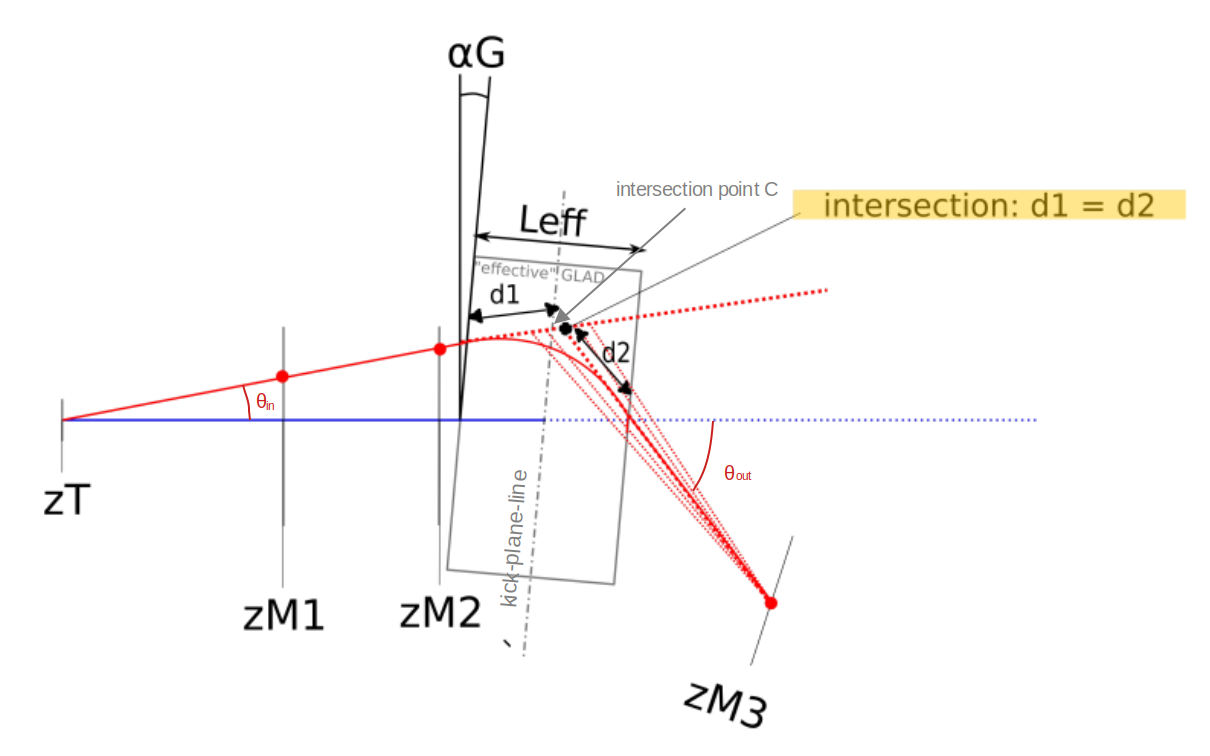
\includegraphics[width=\textwidth]{Figures/kick_point_algorithm.png}
        \caption{Flightpath reconstruction with "Leff" being the effective active width of the magnetic field of GLAD}
        \label{fig:sub1_reco_path}
    \end{subfigure}
    %\hfill % Optional: adds horizontal space between the figures
    % Second subfigure
    \begin{subfigure}[b]{0.25\textwidth}
		\centering
        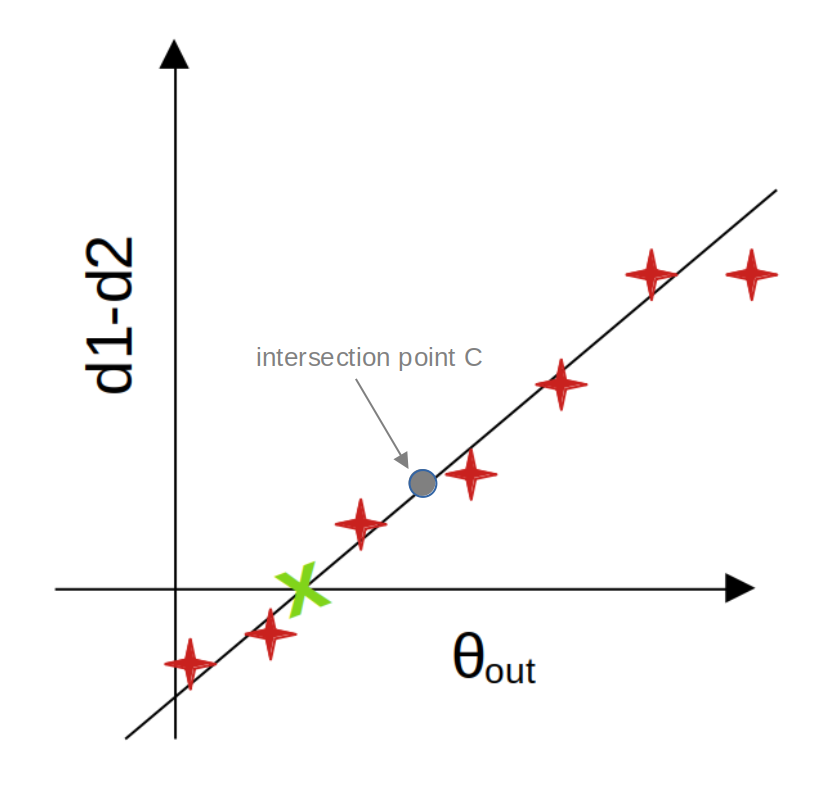
\includegraphics[width=\textwidth]{Figures/intersection_algorithm.png}
        \caption{$\theta_{out}$ approximation. For detailed information see text.}
        \label{fig:sub2_reco_path}
    \end{subfigure}

    \caption{Flightpath tracking and reconstruction of the fragment/beam after the target.}
    \label{fig:reco_path}
\end{figure}

Now that the scattering angle after the target $\theta_{in}$ and the angle after GLAD, $\theta_{out}$ is known and the position outside the magnetic field of GLAD are fixed, with $(z_1,x_1)$  the entrance point on the GLAD field and $(z_2,x_2)$ the exit point, the bending radius $r$ from the magnetic deflection can be determined:
\begin{equation}\label{eq:rho_glad}
r = \frac{L_{eff}}{2\,\cdot sin\left(\frac{\theta_{in}+\theta_{out}}{2}\right)\,\cdot cos\delta}
\end{equation}
where $L_{eff}$ is the effective active with of the magnetic field of GLAD, which correspons $L_{eff} \approx 2.06\,m$. This value could also be verified by extracting $L_{eff}$ from the formula for the magnetic rigidity $ B\cdot r = \gamma\beta \, m /q$ for empty target runs with known values of the B-field\footnote{For detector calibration, primarly for the ToFWall, we had several "empty sweep runs", with empty target and different B-field strenght settings. Those runs were optimal to validate $L_{eff}$.}.\newline
The angle $\delta$ in equation \ref{eq:rho_glad} is given by the trajectory line going through $(z_1,x_1)$/$(z_2,x_2)$ and the line parallel to the GLAD magnet width $L_{eff}$.\newline
A detailed derivation of equation \ref{eq:rho_glad} can be found in appendix \ref{app:flightpath}.
The arc trajectory $l_{GLAD}$ of the fragment within GLAD can be reconstructed using the bending radius $r$ and the entry and exit points $(z_1,x_1)$/$(z_2,x_2)$:
\begin{equation}\label{eq:arc}
l_{GLAD} = r \cdot \omega\qquad \text{with}\qquad \omega = 2\cdot asin(t_{1/2}{(2\cdot r)})
\end{equation}
where $\omega$ is the central angle and  $t_{1/2}$ is the cord length between $(z_1,x_1)$ and $(z_2,x_2)$.\newline
At this stage the full pathlength $L$ form the Start detector to the ToFW is fixed:
\begin{description}
\item \textbf{From Start to the target $l_{ST}$:} For this path section a straight flightpath parallel to the z-coordinate is assumed. The pathlength is taken from the position measurements of the Start detector and the target accordingly ($=118.3\,cm$). 
\item \textbf{Target to GLAD entrance point $(z_1,x_1)$, $l_{in}$:}For the  exact position assignment of $(z_1,x_1)$ both MWPC1 and MWPC2 position measurements have been calibrated with empty target runs by including an offset valuein order to center the x-position in both detectors around zero. From the position measurement of the central position of GLAD, its tilting angle $\alpha$ and $L_{eff}$ the intersection point of the fragment trajectory before GLAD and the "effective GLAD magnetic field rectangle", $(z_1,x_1)$, can be determined and with it the according flightpath section $l_{in}$.
\item \textbf{Arc trajectory within GLAD, ${l_{GLAD}}$:}This flightpath passage is determined by reconstructing $(z_1,x_1)$ and $(z_2,x_2)$, as it has been described in detail in the previous section. Hence the magnetic bending radius can be determined, see equation \ref{eq:rho_glad}, and finally the arc trajectory ${l_{GLAD}}$ as in equation \ref{eq:arc}.
\item \textbf{GLAD exit point $(z_2,x_2)$ to ToFW, $l_{out}$:}The hit position $(z_{MWPC3},x_{MWPC3})$ in MWPC3 is given by the reconstructed hit position in this detector and the position measurement of the detector itself. The exit point $(z_2,x_2)$ was reconstructed in the previous steps. Hence the trajectory line from $(z_2,x_2)$ to $(z_{MWPC3},x_{MWPC3})$ is fixed and is expanded to the intersection with the ToFW plane for the concluding $l_{out}$ measurement.  
\end{description}
The resulting flightpath $L$ recombines from:
\begin{align*}
L &= l_{ST}+l_{in}+l_{GLAD} + l_{out} 
\end{align*}
In the flightpath reconstruction the deflections in the y-dimension were omitted as the angular straggling in the target is small (TODO: give sigma value) and since the deflection of the fragment within GLAD is independent from its  y-position this contribution can be disregarded.


\subsubsection{Time of Flight Calibration}
For the time of flight measurement in the S444 setup the time is recorded and digitized by the VFTX,  VME-FPGA Time-to-Digital Converter (TDC) Modules based on tapped delay line (TDL) TDCs\cite{bayer2009development}. These modules provide for each detected signal a coarse time, is determined by counting cycles of a 200 MHz readout clock, resulting in a 5 ns binning resolution, and a fine time, which is obtained using an FPGA-based Time-to-Digital Converter (TDC), which employs a tapped delay line (TDL). In this approach, the signal propagates through a series of delayed logic modules within the FPGA until the subsequent clock cycle terminates the sampling process. The number of delay elements traversed by the signal is used to compute the time difference between the signal onset and the end of the clock cycle. The translation of the resulting fine time, with reasonable assumption of an uniform distribution, is achieved via a calibrated linear function. This procedure assigns to each preamplifier signal in the start detector (left/right) and the ToF Wall (up/down) a calibrated raw time \textit{raw\_t}:
\begin{align*}
raw\_t &= coarse\_time\_clocks  \cdot 5ns + offset[fine\_time]
\end{align*}
Finally, the raw time of flight is reconstructed by combinding all four time measurements:
\begin{gather}
RawTof = 0.5*(raw\_t_{i,down}+raw\_t_{i,up}) - 0.5*(raw\_t_{start,right}+raw\_t_{start,left})
\end{gather}
where \textit{i} $(\in 0...27)$ refers to the scintillator number of the ToF Wall. Since the mentioned time measurements are standalone and not synchronized the \textit{RawToF} has to be corrected by an offset which has to be determined again for each scintillator bar \textit{i} of the ToF Wall:
\begin{align*}
\Delta_{ToF}[i] &= \overline{L[i]}/v_{beam} - \overline{RawTof[i]}
\end{align*} 
where $\overline{L[i]}$ is the mean reconstructed path length for all events in empty target runs which hit scintillator bar \textit{i} of the ToF Wall. The beam velocity $v_{beam}$ is directly taken from the given beam settings, e.g. 400 AMeV beam, emtpy target corresponds to $v_{beam} = 214,2mm/ns$. The mean raw ToF $\overline{RawTof[i]}$ again results from all events which hit scintillator bar \textit{i} and is extracted from the mean value of a gaussian fit to the raw ToF. The resulting calibrated ToF can then be expressed as:
\begin{align*}
ToF[i] = 0.5*(raw\_t_{i,down}+raw\_t_{i,up}) - 0.5*(raw\_t_{start,right}+raw\_t_{start,left}) + \Delta_{ToF}[i]
\end{align*}  
To estimate the time of flight resolution for events with hit in ToF Wall bar \textit{i} it has to be noted that the ToF is affected by the flight path. Hence the the time of flight should be written as:
\begin{align*}
%ToF &= \frac{$\overline{L[i]}$}{\frac{L[i]}{ToF[i]}}
\widetilde{ToF} &= \frac{\overline{L[i]}}{\frac{L[i]}{ToF[i]}}
\end{align*}
$\overline{L[i]}$ is the mean pathlength, whereas $L[i]$ and $ToF[i]$ are eventwise selected.
By reconstructing the fligh-path as described in subsection \ref{subsec:flightpath_reco} and employment of the mentioned time calibration steps the average time resolution $\sigma_t$ results $\approx 90\, ps$\footnote{To remove events with large angular straggling, a cut of $\pm 20mm$ on the beam spot for the y-position on the MWPC3 was applied.}.

\subsection{Event Selection}
For the precise measurement of the total interaction cross section $^{12}C + ^{12}C$, as detailed in the section \ref{sec:analysis_cross_sec}, event selection was of critical importance, requiring stringent cuts on the TPats (see table \ref{tab:tpats}), as well as on the charge and position of the incoming particles. In contrast, for this qualitative QFS analysis, these factors played a minor role, allowing for only minimal cuts on the incoming ions:
\begin{itemize}
\item Both left and right preamplifiers of the start detector have seen a coincident signal.
\item Exactly one hit in MWPC0 in the hit-level data.
\end{itemize}
However, for the identification of fragments downstream of the target, various detector signals and event parameters are required:
\begin{itemize} 
\item One hit (in the hit-level data) in the MWPC tracking detectors, MWPC1 and MWPC2 upstream to GLAD, MWPC3 downstream to GLAD.
\item Charge measurement in the TWIN-MUSIC.
\item One hit scintillation bar in ToF Wall with signal from both up/down PMTs.
\end{itemize}
\subsection{Fragment Identification}\label{sec:frag_ident}
The first step for the identification of the QFS-reaction channel $^{12}C(p,2p)^{11}B$ is the identification of the fragment $^{11}B$ via the formula for the magnetic rigidity: $ B\cdot r = \gamma\beta \, m /q$ where the $\gamma$ factor accounts for the increase in momentum for relativistic particles. From the flightpath reconstruction and the ToF measurement as described in previous sections $r$,$\beta$ and $\gamma$ are obtained whereas the charge of the fragment $q$ is measured by the energy loss ($\Delta E \sim Z^2$) in the TWIN MUSIC detector.\newline
The measured values for $\frac{A}{q}$ and $q$ are shown in figure \ref{fig:a_q_vs_q} where the fragment of interest $^{11}B$ is expected to be at $\frac{A}{q} = 11/5 \approx 2.2$ and $q = 5$. The correlation plot exhibits a broad distribution in $\frac{A}{q}$, which may result from misidentification of hit positions in one of the MWPC tracking detectors when multiple signal hits occur. Even minor deviations in MWPC1 and MWPC2 can significantly affect the radius reconstruction, thereby impacting the accuracy of the $\frac{A}{q}$ determination.\newline
An intriguing feature is the distinct cluster observed at $Z \approx 8.5$ and $\frac{A}{q} \approx 2$, which corresponds to pileup events. These occur when two ion signals arrive within a short time window in the TWIN MUSIC detector, preventing them from being resolved as separate events and instead being reconstructed as a single signal\footnote{For instance, if two carbon ions ($Z=6$) interact simultaneously, the total energy loss within TWIN MUSIC is approximately twice that of a single ion. Since the energy loss follows the relation $\Delta E \sim Z^2$, the reconstructed charge is given by $\sqrt(2)\,Z_{carbon} \approx 8.5 $.}.
Moreover attention should be paid that it seems to be there a cut from analyis side at $Z \approx 4$. This is actually not the case. The TWIM MUSIC was optimized for the subsequent experimental run S467 with $Ca$ isotopes and herefore the charge measurement was optimized for $Z\approx 20$. Everything below $Z \approx 4$ was below the signal threshold of TWIM MUSIC.

Furthermore, it is important to note the apparent cut at $Z \approx 4$ in the data. However, this is not an artifact of the analysis but rather a consequence of the experimental setup. The TWIN MUSIC detector was optimized for the subsequent S467 experiment, which focused on calcium isotopic chain ($Z = 20$). As a result, the charge measurement was calibrated for $Z \approx 20$, and signals corresponding to $Z \lesssim 4$ fell below the detection threshold of TWIN MUSIC.

\begin{figure}[htpb]
    \centering
    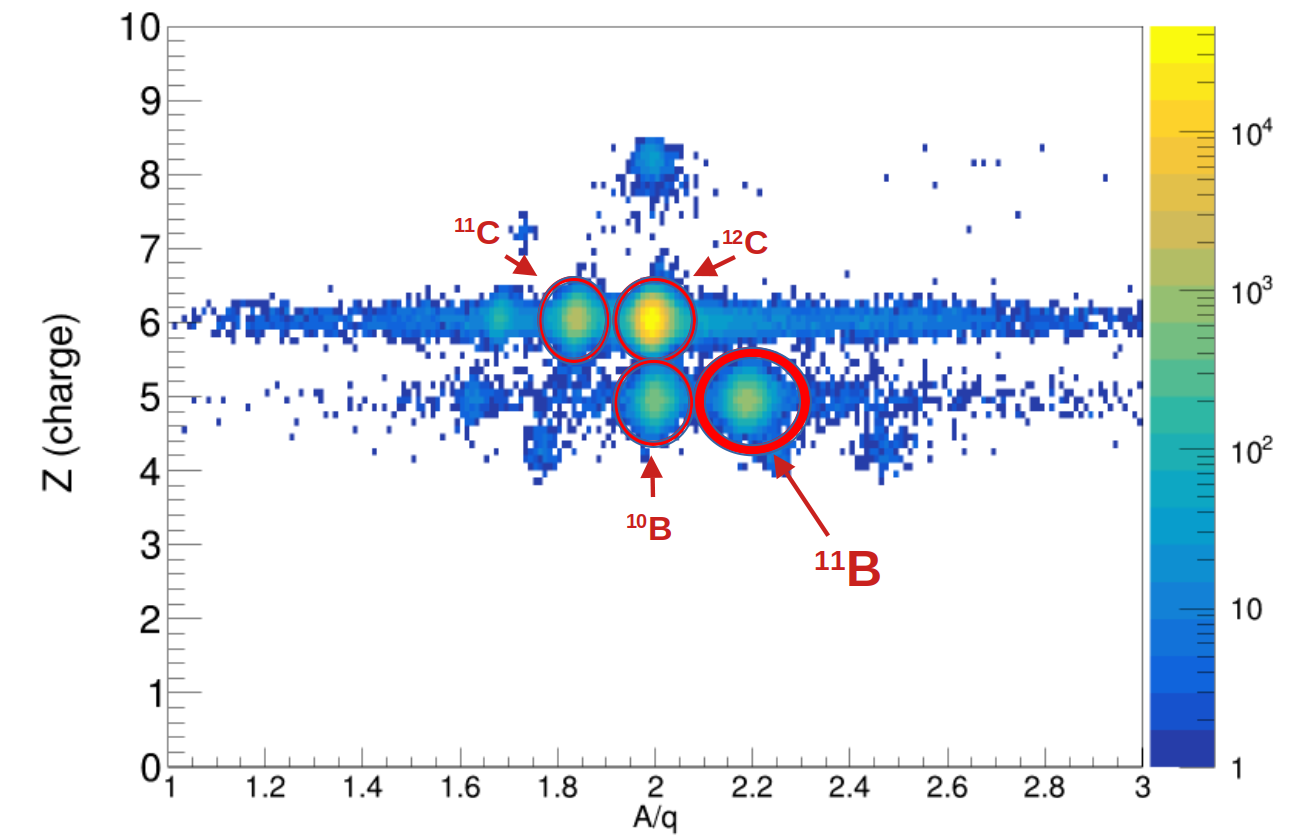
\includegraphics[width=\textwidth,height=12cm,keepaspectratio=true]{Figures/a_over_q_vs_q_plot.png}
    \caption{
	Fragment identification is performed using the correlation between the atomic number $Z$ and the mass-to-charge ratio $\frac{A}{q}$. For the quasi-free scattering (QFS) analysis of the reaction $^{12}C(p,2p)^{11}B$, the fragment of interest is $^{11}B$, which is emphasized with a bold red circle.
    }
    \label{fig:a_q_vs_q}
\end{figure}
For this qualitative analysis, the upper charge bound of $^{11}B$ was determined by locating the intersection point of the Gaussian-fitted distributions corresponding to the $Z=5$ and $Z=6$ peaks. The lower bound was set by applying an offset of minus one unit.\newline
A similar approach was employed to select the specific boron isotope $^{11}B$. The charge selection was performed using the previously defined boundary cuts. To isolate the $^{11}B$ isotopes, the lower bound was determined by identifying the intersection point of the Gaussian-fitted distributions corresponding to the $^{10}B$ and $^{11}B$ peaks. The upper bound was established by measuring the distance from this intersection point to the peak of $^{11}B$.

\subsection{QFS-Protons}\label{sec:qfs_protons}
Following the identification of the fragments through precise flight path reconstruction and time measurement, as detailed in the previous subsection, and the subsequent selection of the $^{11}B$ isotope, the analysis focuses on the two correlated protons to fully characterize the quasi-free scattering channel $^{12}C(p,2p)^{11}B$.\newline
For a proper interpretation of the data, it is essential to consider the geometric acceptance of CALIFA during the S444 experiment in 2020. The central \textit{BARREL} region (Ring 3 and Ring 4), covering the polar angular range from $43^{\circ}$ to $88^{\circ}$, was fully operational. In contrast, the forward region, referred to as \textit{iPhos} ($19^{\circ}$ to $43^{\circ}$), was only partially equipped, with a coverage of approximately $35\%$. The forward endcap, known as \textit{CEPA}, was not installed, and the backward barrel remained unoccupied. The corresponding geometry is illustrated in figure \ref{fig:qfs_reac_and_geo}.\newline
\begin{figure}[htpb]
	\begin{subfigure}[t]{.4\linewidth}
    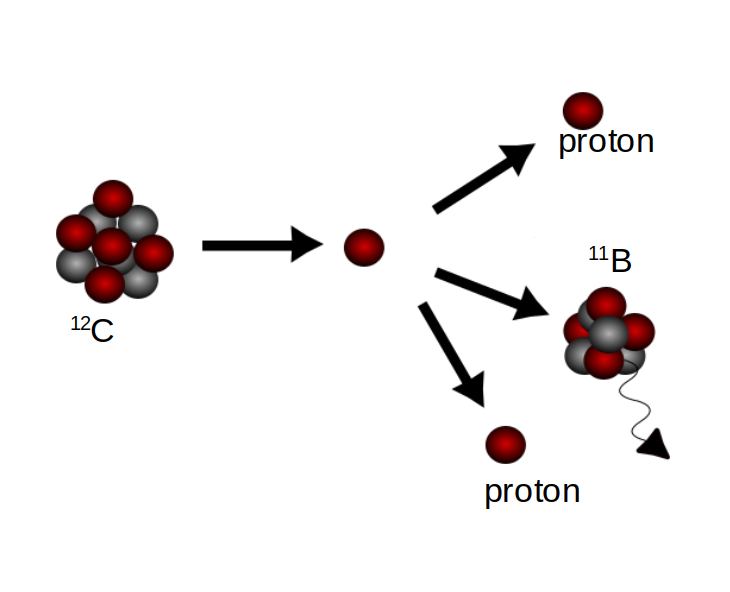
\includegraphics[width=\textwidth]{Figures/reaction_qfs_model.png}
	\caption{Quasi-free scattering channel $^{12}C(p,2p)^{11}B$}
	\end{subfigure}
	\begin{subfigure}[t]{.4\linewidth}
    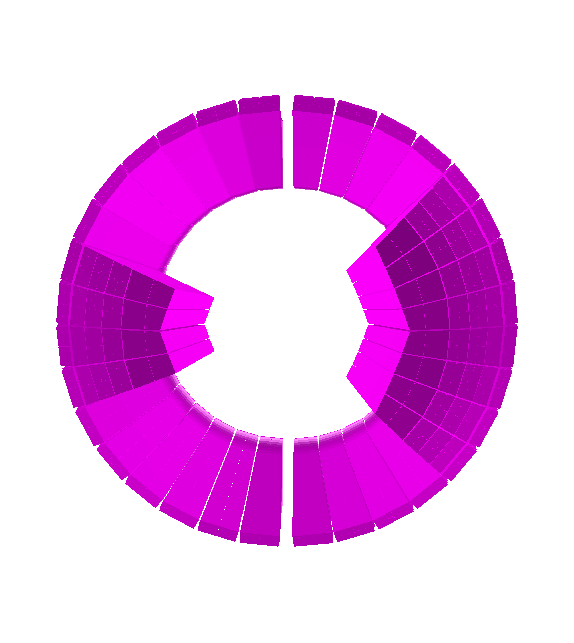
\includegraphics[width=\textwidth]{Figures/CALIFA2020Front.png}
	\caption{Simulated front view of the CALIFA calorimeter in 2020.}
	\end{subfigure}
    \caption{Tagging the $^{12}C(p,2p)^{11}B$ channel with only partly filled CALIFA calorimeter for the detection of the two correlated protons.}%
    \label{fig:qfs_reac_and_geo}%
\end{figure}
For the proton selection and the application of reasonable cuts it is important to understand the processing steps of the raw \textit{mapped} level data to the \textit{cal} level and finally \textit{hit} level data. The \textit{mapped} level data has following structure for each CALIFA hit:
For an accurate proton selection and the application of appropriate cuts, it is crucial to understand the data processing steps from the raw \textit{mapped}-level to the \textit{cal}-level and finally to the \textit{hit}-level. The \textit{mapped}-level data for each CALIFA hit is structured as follows:
\begin{itemize}
\item[$\blacksquare$] CrystalID: each crystal channel gets assigned a unique ID. Gamma range channels are in the range up to 2550, proton range ones from 2550 up to ..
\item[$\blacksquare$] Uncalibrated Energy
\item[$\blacksquare$] Slow Component $N_s$, extracted from the signal shape, see \cite{winkel2011implementierung}, section 2.
\item[$\blacksquare$] Fast Component $N_f$, extracted from the signal shape, see \cite{winkel2011implementierung}, section 2.
\item[$\blacksquare$] WRTS: White Rabbit Time Stamp\cite{serrano2013white}, interpolated from FEBEX inner clock.
\item[$\blacksquare$] Time over Threshold, optionally activated for $\gamma$-range channels to reconstruct energies beyond range.
\end{itemize}

The \textit{cal}-level data is structured as in the \textit{mapped}-level, however with calibrated energy by applying the calibration parameters from calibration run to each crystal channel.\newline
For the calibration runs a $^{22}Na$ (with peaks at $511keV$ and $1275keV$) or a $^{60}Co$ (with peaks at $1173keV$ and $1332keV$) source is used. For each crystal channel a linear fit on the two photopeaks is performed. Using this fitting function, the uncalibrated energy, expressed in energy channels, can be converted into calibrated energy values.\newline
For the final \textit{hit}-level data, the energy-calibrated hits from the \textit{cal}-level are merged into clusters. High-energy proton hits ($E_{hit} > 15 MeV$) and low-energy $\gamma$ hits are first listed and sorted in descending energy order. Clusters are then formed using a cone-shaped approach, where each cluster is centered around the highest-energy hit with a half-opening angle of $\theta_c = 14.3^{\circ}$. All hits within this angular region are merged into the cluster. This process is iteratively repeated until both the high- and low-energy lists are empty. To improve the signal-to-noise ratio in this analysis, hits with energy values below the threshold of $E_{thr} = 100keV$ are discarded during clustering.\newline
The resulting correlations in azimuthal and polar angles,with the only cut to have at least two high energy clusters with energy larger 15 MeV, with respect to the simulated \textit{p2p}-simulations are shown in figure \ref{fig:azimuth_corr} and figure \ref{fig:polar_corr} accordingly.\newline
\begin{figure}[htpb]
	\begin{subfigure}[t]{.75\linewidth}
    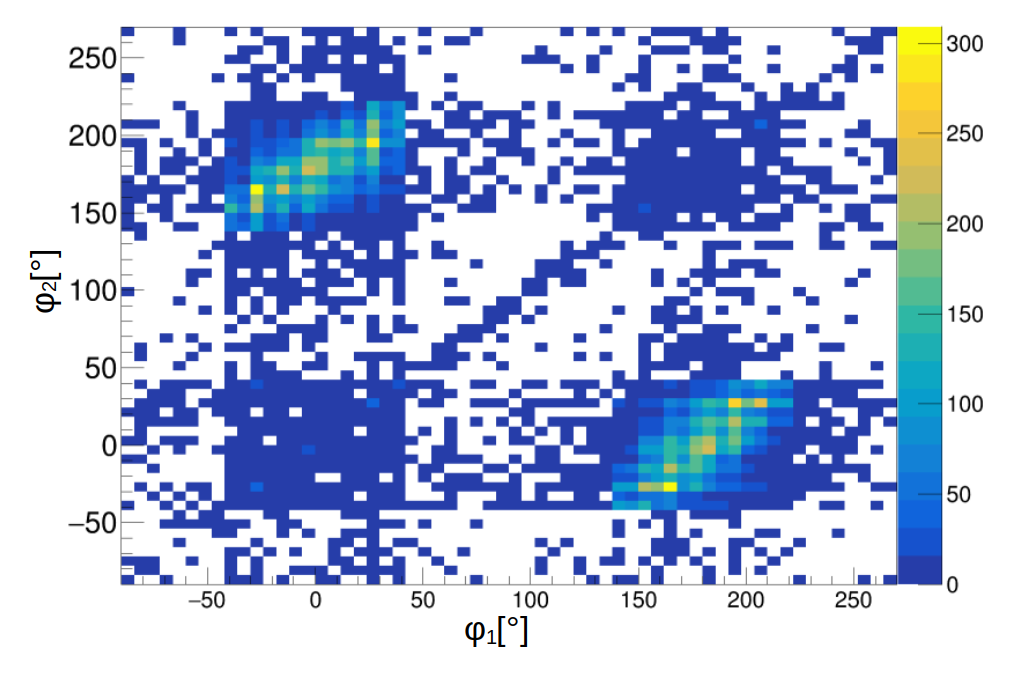
\includegraphics[width=\textwidth]{Figures/phi12_califa.png}
	\caption{Correlation from S444 experimental data}
	\end{subfigure}
	\begin{subfigure}[t]{.75\linewidth}
    \includegraphics[width=\textwidth]{Figures/phi12_sim.png}
	\caption{Simulated data using based on QFS kinematical code by Leonid Chulkov, GSI.}
	\end{subfigure}
    \caption{Azimuthal angular correlation $\varphi_1$ versus $\varphi_2$ of the two clusters with highest energy in CALIFA }
    \label{fig:azimuth_corr}
\end{figure}
From the azimuthal correlation plot in Figure \ref{fig:azimuth_corr}, the geometric acceptance limitations of CALIFA become evident. In the so-called \textit{iPhos} region, CALIFA was instrumented only within the azimuthal ranges of $\pm 45^{\circ}$ and $157.5^{\circ}$ to $202.5^{\circ}$. Due to relativistic kinematics, both protons undergo a forward boost, leading to their predominant detection in the iPhos array. Consequently, any acceptance loss in this region has a substantial impact on the overall detection efficiency.\newline
Moreover, the correlation plot exhibits a distinct correlation line at $\varphi_1 \approx \varphi_2$. This feature primarily arises from inaccuracies in cluster reconstruction, where proton cluster hits fall outside the predefined cone size of the reconstruction algorithm, resulting in the erroneous identification of two separate hits. This effect is particularly pronounced in the \textit{iPhos} region as it is the primary detection region for the protons. Such misidentified events are systematically excluded in analyses focusing on the clean $^{12}C(p,2p)^{11}B$ channel.\newline
\begin{figure}[htpb]
	\begin{subfigure}[t]{.75\linewidth}
    \includegraphics[width=\textwidth]{Figures/theta12_califa.png}
	\caption{Correlation from S444 experimental data}
	\end{subfigure}
	\begin{subfigure}[t]{.75\linewidth}
    \includegraphics[width=\textwidth]{Figures/theta12_sim.png}
	\caption{Simulated data using based on QFS kinematical code by Leonid Chulkov, GSI.}
	\end{subfigure}
    \caption{Polar angular correlation $\theta_1$ versus $\theta_2$ of the two clusters with highest energy in CALIFA }
    \label{fig:polar_corr}
\end{figure}
The polar angular correlation in figure \ref{fig:polar_corr} shows as expected a strong anti-correlation between the two proton clusters. For beam energies up to approximately $500 AMeV$ the anti-correlation line is expected to be uniformly distributed over the polar range as the momentum transfer $t = -Q^2$, which defines the angular distributions $\theta_{1/2}$, does not effect the cross section in this energy regime\footnote{At higher beam energies, parameterizations of the cross section as a function of $t$ often take the form $\frac{d\sigma}{dt} = C e^{bt}$, where $C$ and $b$ are empirically determined parameters.}.\newline
Moreover in figure \ref{fig:polar_corr} the two off-diagonal lines should be noted. This artifact arises from wrong cluster reconstruction where proton cluster hits fall outside the predefined cone size of the reconstruction algorithm, resulting in the erroneous identification of two separate hits. As the resulting clusters are in close proximity, they exhibit a systematic offset from the diagonal in the polar angular correlation plot.\newline
The information of azimuthal and polar angles of the two protons can merged in the opening angle of the two reconstructed protons via the geometric formula:
\begin{equation}\label{eq:opang}
\theta_{p2p} = acos\left( \sin(\theta_1) \sin(\theta_2) \cos(\varphi_2 - \varphi_1) + \cos(\theta_1) \cos(\theta_2) \right)
\end{equation}

\begin{figure}[htpb]
	\begin{subfigure}[t]{.43\linewidth}
    \includegraphics[width=\textwidth]{Figures/opang.png}
	\caption{Opening angle distribution from S444 experimental data}
	\end{subfigure}
	\begin{subfigure}[t]{.47\linewidth}
    \includegraphics[width=\textwidth]{Figures/opang_sim.png}
	\caption{Simulated opening angle $\theta_{p2p}$ based on QFS kinematical code by Leonid Chulkov, GSI.}
	\end{subfigure}
    \caption{Reconstruction of the opening angle $\theta_{p2p}$ as in equation \ref{eq:opang} from the two clusters with highest energy in CALIFA }
    \label{fig:opang}
\end{figure}

Figure \ref{fig:opang} presents the opening angle $\theta_{p2p}$ for the reconstructed protons. In both the simulated and experimental data, the distribution exhibits a peak at approximately $81^{\circ}$. While the simulated distribution shows a strict upper limit around $82^{\circ}$, the experimental data features a pronounced tail extending toward larger values. This effect is primarily attributed to final-state interactions (FSI) and can be significantly reduced by applying appropriate selection criteria to the polar and azimuthal angular correlations of the two reconstructed high-energy hits.\newline
Herefore in the next considerations only events with following criteria are selected:
\begin{itemize}
\item $\theta_1 + \theta_1 < 90^{\circ}$
\item $\Delta \varphi < 180 \pm 40^{\circ}$
\end{itemize}

\subsubsection{Missing Momentum $\mathbf{p_{miss}}$ Reconstruction}\label{sec:p_miss}

As discussed in Section \ref{sec:qfs_theo}, the momentum of the knocked-out proton inside the $^{12}C$ nucleus can be reconstructed, assuming higher-order perturbations are negligible, as described by Equation \ref{eq:miss_mom}. For this reconstruction, the momenta of the two detected protons, $\mathbf{p_{1/2}}$, and the initial target proton, $\mathbf{p_{0}}$ (which is approximately zero in the laboratory frame), must be known and transformed into the center-of-mass frame of the $^{12}C$ nucleus. The resulting distribution of the missing momentum, $\mathbf{p_{miss}}$, obtained from experimental data, is presented in Figure \ref{fig:p_miss}.\newline
\begin{figure}[htpb]
    \centering
    % Large subfigure
    \begin{subfigure}[b]{0.9\textwidth}
        \centering
        \includegraphics[width=\textwidth]{Figures/p_miss_tot.png} % Replace with your image file
        \caption{Reconstructed absolulte value of $\mathbf{p_{miss}}$.}
        \label{fig:p_miss_tot}
    \end{subfigure}

    % Row of three smaller subfigures
    \begin{subfigure}[b]{0.3\textwidth}
        \centering
        \includegraphics[width=\textwidth]{Figures/p_miss_x.png} % Replace with your image file
        \caption{Reconstructed\newline x-component of $\mathbf{p_{miss}}$.}
        \label{fig:p_miss_x}
    \end{subfigure}
    \begin{subfigure}[b]{0.3\textwidth}
        \centering
        \includegraphics[width=\textwidth]{Figures/p_miss_y.png} % Replace with your image file
        \caption{Reconstructed\newline y-component of $\mathbf{p_{miss}}$.}
        \label{fig:p_miss_y}
    \end{subfigure}
    \begin{subfigure}[b]{0.3\textwidth}
        \centering
        \includegraphics[width=\textwidth]{Figures/p_miss_z.png} % Replace with your image file
        \caption{Reconstructed\newline z-component of $\mathbf{p_{miss}}$.}
        \label{fig:p_miss_z}
    \end{subfigure}

    \caption{Reconstructed $\mathbf{p_{miss}}$ and its components in the $^{12}C$ rest frame}
    \label{fig:p_miss}
\end{figure}

Compared to previous experimental results, such as those reported in Ref. \cite{moniz1971nuclear}, where the measured Fermi momentum for $^{12}C$ was determined to be $221 \mp 5$ MeV/c, corresponding to a mean internal proton momentum of $171$ MeV/c, the reconstructed mean value in the present analysis is found to be $156$ MeV/c.\newline
While this value is slightly lower than the reference, it is important to consider the specific experimental conditions. The geometric acceptance of CALIFA, particularly in the forward region, was not fully instrumented, which may introduce some distortions in the reconstructed $\mathbf{p_{miss}}$ distribution. Nevertheless, the obtained results remain consistent within the expected systematic uncertainties.\newline
Furthermore, the beam energy, assumed to be constant at $400, A\text{MeV}$, plays a crucial role in transforming the reconstructed proton momenta into the center-of-mass frame of the $^{12}C$ nucleus. Small variations in the actual beam energy could have a non-negligible impact on the missing momentum reconstruction. Since no precise event-by-event beam energy information was available for this analysis, a constant value of $400$ AMeV was used.\newline
Additionally, as shown in Figure \ref{fig:p_miss_z}, the distribution of the z-component of $\mathbf{p_{miss}}$ exhibits a slight asymmetry, with a tail extending toward lower values. Since the z-component is particularly sensitive to deviations in the mean beam energy, this effect further contributes to the shift of the mean $\mathbf{p_{miss}}$ value toward lower values. Future studies with improved acceptance corrections and access to event-wise beam energy measurements could further refine the results and enhance the accuracy of the $\mathbf{p_{miss}}$ reconstruction.


\subsubsection{Correlations between $^{11}B$ Fragment and the reconstructed inner Proton }
%In subsection \ref{sec:p_miss} we reconstructed the momentum of the inner proton $\mathbf{p_{miss}}$. Herefore only data from the CALIFA calorimeter was necessary. As next step the reconstructed inner proton momentum $\mathbf{p_{miss}}$ can be correlated with the reconstructed $^{11}B$ momentum in the $^{12}C$ rest frame. The momenta of the two constituents of the $^{12}C$, the reconstruced proton and the $^{11}B$, should add up to zero since this is the definition of the rest frame. That means that the momentum vectors of the inner proton and the $^{11}B$ accordingly should point to opposite directions. Which again means for the cosine of the angle $\gamma$ between the two constituents should be approximately -1. This is also what we receive from data, as shown in figure \ref{fig:cos_gamma}.\newline
%Moreover figure \ref{fig:x_corr_p_miss_11b} and \ref{fig:y_corr_p_miss_11b} show the correlation between the x and y momentum of the inner proton to the accoring component of the $^{11}B$ accordingly. In both cases a strong anti-correlation is visible. While the correlation plot for the y component is relatively sharp, the one for the x component is quite blurred. This really comes from the geometric dependent resolutions in the subdetectors:\newline
%For the x component it has to be considered that only the side halves of CALIFA are filled in the \textit{iPhos} region ($\varphi_{1/2}$ in the region $\pm 45^{\circ}$ and $157.5^{\circ}$ to $202.5^{\circ}$). The angular resolution in $\varphi$ is only moderate ($\approx \frac{6^{\circ}}{sqrt{12}}$ and the x component reconstruction is proportional to $\cos(\varphi)$ with an only slowly changing derivative ($\sin(\varphi)$) for $\varphi \approx 0$. Moreover the x component of the $^{11}B$ fragment has to be reconstructed from the position resolutions right after the target with a small lever arm compared to the reconstruction of the y component of the $^{11}B$ fragment which is reconstructed from the y information in MWCP3 after GLAD, since the y component should not be affected by the GLAD magnet. 
%
In Subsection \ref{sec:p_miss}, the momentum of the inner proton, $\mathbf{p_{miss}}$, was reconstructed using data exclusively from the CALIFA calorimeter. As a next step, this reconstructed momentum can be correlated with the momentum of the $^{11}B$ fragment in the rest frame of the $^{12}C$ nucleus.\newline

Since the total momentum in the rest frame must be zero by definition, the momentum vectors of the inner proton and the $^{11}B$ fragment should be directed oppositely. Consequently, the cosine of the angle $\gamma$ between these two constituents should be approximately $-1$, which is confirmed by the experimental data, as shown in Figure \ref{fig:cos_gamma}.\newline

Furthermore, Figures \ref{fig:x_corr_p_miss_11b} and \ref{fig:y_corr_p_miss_11b} illustrate the correlation between the x- and y-components of $\mathbf{p_{miss}}$ and the corresponding components of the $^{11}B$ fragment. A strong anti-correlation is observed in both cases. While the correlation in the y-component is relatively sharp, the x-component exhibits a more blurred distribution.\newline

This effect arises from the geometry-dependent resolution of the subdetectors:
\begin{itemize}
\item[--]For the x-component, it is important to consider that only the lateral halves of CALIFA were instrumented in the \textit{iPhos} region ($\varphi_{1/2}$ within $\pm 45^{\circ}$ and $157.5^{\circ}$ to $202.5^{\circ}$). The azimuthal resolution is moderate ($\approx \frac{6^{\circ}}{\sqrt{12}}$), and since the x-component is reconstructed as $\propto \cos(\varphi)$, the derivative $\sin(\varphi)$ remains small for $\varphi \approx 0$, leading to lower sensitivity in this region.
\item[--] The x-component of the $^{11}B$ fragment is reconstructed from position measurements immediately after the target, where the lever arm for momentum reconstruction is relatively short.
\item[--]In contrast, the y-component of the $^{11}B$ fragment is determined from its position in MWPC3 after GLAD, where the larger lever arm improves resolution. Moreover, the y-component remains largely unaffected by the GLAD magnet, further enhancing its reconstruction accuracy.
\end{itemize}

\begin{figure}[!htb]
    \centering
    % Large subfigure on the left
    \begin{subfigure}[b]{0.9\textwidth}
        \centering
        \includegraphics[width=\textwidth]{Figures/cos_angle_2p_11b.png} % Replace with actual image
        \caption{Cosine of the angle $\gamma$ between inner proton and $^{11}B$.}
        \label{fig:cos_gamma}
    \end{subfigure}

    \vspace{0.3cm} % Adjust vertical spacing

    % Row for two smaller subfigures
    \begin{subfigure}[b]{0.39\textwidth}
        \centering
        \includegraphics[width=\textwidth]{Figures/p_x_2p_11b.png} % Replace with actual image
        \caption{x-component correlation between inner proton and $^{11}B$.}
        \label{fig:x_corr_p_miss_11b}
    \end{subfigure}
    \hspace{0.2cm} % Adjust horizontal spacing
    \begin{subfigure}[b]{0.39\textwidth}
        \centering
        \includegraphics[width=\textwidth]{Figures/p_y_2p_11b.png} % Replace with actual image
        \caption{y-component correlation between inner proton and $^{11}B$.}
        \label{fig:y_corr_p_miss_11b}
    \end{subfigure}

    %% Small subfigures stacked on the right
    %\begin{subfigure}[b]{0.9\textwidth}
    %    \centering
    %    \begin{subfigure}[b]{0.9\textwidth}
    %        \centering
    %        \includegraphics[width=0.45\textwidth]{Figures/p_x_2p_11b.png} % Replace with actual image
    %        \caption{x-component correlation between inner proton and $^{11}B$.}
    %        \label{fig:x_corr_p_miss_11b}
    %    \end{subfigure}
    %    \vspace{0.2cm}
    %    \begin{subfigure}[b]{0.9\textwidth}
    %        \centering
    %        \includegraphics[width=0.45\textwidth]{Figures/p_y_2p_11b.png} % Replace with actual image
    %        \caption{y-component correlation between inner proton and $^{11}B$.}
    %        \label{fig:y_corr_p_miss_11b}
    %    \end{subfigure}
    %\end{subfigure}
    
    \caption{Correlation plots between inner proton and $^{11}B$ in the $^{12}C$ rest frame.}
    \label{fig:corr_p_miss_11b}
\end{figure}

TODO:->Maybe also correlations between fragment and proton pair, see Chulkov.


\subsubsection{Proton Separation Energy $S_p$}
The proton separation energy $S_p$ of $^{12}C$ from the reaction channel $^{12}C(p,2p)^{11}B$ is defined by the masses and energies of the initial and final state particles in the $^{12}C$ rest frame. One can write the full energy conservation in the rest frame of $^{12}C$:
\begin{equation}
M_{^{12}C} + \gamma \cdot m_p = E_1^* + E_2^* + (M_{^{11}B} + E_{ex})  + T_{^{11}B^*}
\end{equation}
where $E_1^*$ and $E_2^*$ are total energies of the two protons in the $^{12}C$ rest frame, $E_{ex}$ is residual excitation in $^{11}B$ and $T_{^{11}B^*}$ the kinetic energy of the $^{11}B$ in the $^{12}C$ rest frame.\newline
Using this equation, one can express the total binding energy $B$ of the knocked out nucleon:
\begin{equation}
B = S_p - E_{ex} = M_{^{12}C} - M_{^{11}B} - E_{ex} - m_p = E_1^* + E_2^* + T_{^{11}B^*} - \gamma \cdot m_p - m_p
\end{equation}
Using Lorentz transformation from lab to 12C rest frame one can obtain for $E_1^*/E_2^*$:
\begin{align*}
E_{1/2}^* &=  \gamma \cdot m_p + \gamma \cdot T_{1/2} - \beta \cdot \gamma \cdot p_{1/2} \cdot cos(\theta_{1/2})
\end{align*}
The kinetic energy of the $^{11}B$ in the $^{12}C$ rest frame can be written as:
\begin{align*}
T_{^{11}B^*} &= \frac{p_i^2}{2 \cdot M_{^{11}B}}
\end{align*}
with $p_i$ the inner momentum of the proton knocked out of the $^{12}C$ projectile, see equation \ref{eq:miss_mom}.
Putting this in the previous equation one finally gets for the binding energy $B$:
\begin{equation}
B = (\gamma - 1)\cdot m_p + \gamma \cdot (T_1+T_2) - \beta \cdot \gamma \cdot(p_1*cos(\theta_1) + p_2*cos(\theta_2)) + T_{^{11}B}
\end{equation}\label{eq:sep_energy}
For $E_{ex} = 0$, i.e. the fragment $^{11}B$ in the ground state, the binding energy $B$ is equal to the one proton separation energy $S_p$\footnote{Since the $^{11}B$ fragment predominantly remains in its ground state---implying that, in most cases, the outermost protons are removed---the binding energy $B$ and the proton separation energy $S_p$ are used interchangeably, also due to the limited energy resolution.}. \newline
As for the S444 experiment no target detector tracking system was available. Consequently the energies as well as the azimutal ($\varphi$) and polar($\theta$) angles of the two correlated protons had to be fully reconstructed using the CALIFA calorimeter. The calorimeter provided an energy resolution $\frac{\Delta E}{E}(@100MeV) \lesssim 1 \%$, along with angular resolutions of approximately  $\Delta \varphi \approx \frac{6^{\circ}}{\sqrt{12}}$, and $\Delta \theta \approx \frac{2^{\circ}}{\sqrt{12}}$.
The best way to visualize the separation energy $S_p$ id to plot it against the summed energy of the two protons in the $^{12}C$ rest frame as shown in figure \ref{fig:sep_energy}. Two vertical lines are visible. They correspond to the two QFS-reaction types within the $CH_2$ target: the proton within the $^{12}C$ projectile can either scatter on the hydrogen (proton-like) part of on the carbon part of the plastic target. For the first case only the separation energy $S_p$ as derived in equation \ref{eq:sep_energy} is necessary to remove the proton of the projectile within the $^{12}C$ nucleus. In the second case the QFS-reaction is between two protons both bound within a carbon nucleus -- the projectile carbon and the target carbon part. Herefore more energy is needed to free both protons from their nuclear bond. This corresponds to the left vertical line in figure \ref{fig:sep_energy}. It should be noted that the reconstructed one-proton separation energy $S_p$ is shifted with respect to the mean value of $\approx 16 MeV$. For a precise measurement the accurate position of the target and the reaction vertex would be needed, as well as a precise measurement of the kinetic energy of the incoming $^{12}C$ would be required (for the actual measurements the beam energy value was set to $400 AMeV$). 
\begin{figure}[htpb]
    \centering
    \includegraphics[width=\textwidth,height=10cm,keepaspectratio=true]{Figures/sep_energy_vs_sum_energy.png}
    \caption{
	Sum of the kinetic energies of the two correlated protons ($T_1/T_2$) versus the one proton separation energy $S_p$. Since this energy is needed to solve the proton from the nucleus' core, it's valuehas conventionally a negative sign.  	 
    }
    \label{fig:sep_energy}
\end{figure}

\subsection{Reconstruction of excited$ ^{11}$B states}
In order to achieve a complete kinematic reconstruction of the reaction products, the use of the CALIFA detector as a $\gamma$-ray spectrometer in the low-energy regime (down to $E_\gamma \geq 100\,\mathrm{keV}$) is essential. This is particularly relevant for reactions such as $^{12}\mathrm{C}(p,2p)^{11}\mathrm{B}$ in quasi-free scattering (QFS) kinematics. In such cases, it is possible to simultaneously identify and measure the energy of the two correlated protons (as demonstrated in previous sections) as well as detect $\gamma$-rays emitted during the de-excitation of $^{11}\mathrm{B}$ from excited states to its ground state ($3/2^-$).

$\gamma$-ray spectroscopy serves as a sensitive probe for investigating the population of low-lying discrete nuclear states. In the case of exotic nuclei, this allows exploration of previously uncharted excited states. For well-known nuclei such as $^{11}\mathrm{B}$, it provides an opportunity to test theoretical shell-model predictions and extract spectroscopic factors with high precision. The established level scheme of $^{11}\mathrm{B}$ is illustrated in Figure~\ref{fig:11B_levels}.
\begin{figure}[htpb]
    \centering
    \includegraphics[width=\textwidth,height=8cm,keepaspectratio=true]{Figures/levelschemaplot.png}
    \caption{
Level scheme of $^{11}\mathrm{B}$ taken from~\cite{iaea_nuclide_chart}.
    }
    \label{fig:11B_levels}
\end{figure}

Assuming the ground-state proton configuration of $^{12}\mathrm{C}$ as $(s_{1/2})^2(p_{3/2})^4$, the removal of a single proton from the $p$-shell is expected to result in a hole state with quantum numbers corresponding to either $3/2^-$ or $1/2^-$. The population of higher angular momentum states is strongly suppressed due to the absence of significant contributions from indirect two-step processes and the limiting influence of ground-state correlations in $^{12}\mathrm{C}$~\cite{van1988weak}.

Some excited states of $^{11}\mathrm{B}$, such as the $5/2^-$ state with a known transition energy of 4.4~MeV, are not expected to be populated under QFS conditions. This state arises from the coupling of angular momenta of multiple unpaired nucleons (e.g., two nucleons in the $p_{3/2}$ orbital coupled to $J_{12} = 2$, and a third nucleon in $p_{1/2}$ with $J_3 = 1/2$). The population of such states via a QFS reaction would contradict the fundamental mechanism of QFS, which involves the interaction of the probe (typically a proton) with a single nucleon, while the remaining $A-1$ nucleons act as spectators.

As the $^{11}\mathrm{B}$ fragments produced in the reaction carry nearly the full beam energy and move predominantly in the forward direction, the emitted $\gamma$-rays from their de-excitation experience relativistic Doppler shifts. Therefore, Doppler correction must be applied to the measured $\gamma$-ray energies. Following standard textbooks (e.g.,~\cite{krane1987}), the relation between the observed $\gamma$-ray energy in the laboratory frame and the rest-frame energy of the emitting nucleus is given by:

\begin{equation}
    E_\gamma = E_0 \cdot \gamma \cdot (1 - \beta \cos \theta)
	\label{eq:doppler}
\end{equation}

where $E_0$ is the intrinsic $\gamma$-ray energy in the rest frame of $^{11}\mathrm{B}$ (approximately the same as the rest frame of the incoming $^{12}\mathrm{C}$), $\gamma = 1/\sqrt{1 - \beta^2}$ is the Lorentz factor, $\beta = v/c$ is the velocity of the $^{11}\mathrm{B}$ fragment normalized to the speed of light, and $\theta$ is the polar angle of the emitted $\gamma$-ray with respect to the beam axis in the laboratory frame\footnote{Since the excited state $1/2^-$ of $^{11}\mathrm{B}$ has a lifetime $T_{1/2} = 3.8$fs (which corresponds to a width of $\Gamma = 0.117$eV, see level scheme in Fig.~\ref{fig:11B_levels}) it is an immediate transition already occurring in the target region.}.\newline
The high granularity of the CALIFA calorimeter enables a precise determination of the emission angle $\theta$ of detected $\gamma$-rays. For each $\gamma$-ray event, the angle $\theta$ is defined by the position of the individual crystal within the $\gamma$-cluster that recorded the maximum deposited energy. This crystal is assumed to represent the most probable direction of the primary $\gamma$-ray emission. The angle is then used--relative to the known target position--to perform the Doppler correction and reconstruct the rest-frame $\gamma$-ray energy $E_0$, according to the relativistic transformation described in Eq.~\eqref{eq:doppler}.
\begin{figure}[htpb]
    \centering
    \includegraphics[width=\textwidth,keepaspectratio=true]{Figures/gamma_spec_12c_p2p_11b.png}
    \caption{
Doppler-corrected $\gamma$-ray spectrum in coincidence with the $^{12}\mathrm{C}(p,2p)^{11}\mathrm{B}$ quasi-free scattering reaction. The prominent peak at $E_{\gamma} \approx 2.1\,\mathrm{MeV}$ corresponds to the de-excitation of the $^{11}\mathrm{B}$ nucleus from its first excited state ($1/2^-$) to the ground state. This peak is fitted with a Gaussian function (blue), while the underlying background is described by an exponential distribution (green). A broader and less well-defined structure is observed at $E_{\gamma} \approx 5\,\mathrm{MeV}$, associated with the de-excitation of the $3/2^-$ state.
    }
    \label{fig:gamma_spec_12c_p2p_11b}
\end{figure}
The resulting Doppler-corrected $\gamma$-ray spectrum is presented in Figure~\ref{fig:gamma_spec_12c_p2p_11b}, which was obtained after applying the following reaction selection criteria:
\begin{itemize}
  \item Identification of the $^{11}\mathrm{B}$ fragment via time-of-flight measurements between the START detector and the TOFW (Sofia), as detailed in Section~\ref{sec:frag_ident}.
  \item Detection of two high-energy hits corresponding to protons, each with an energy deposition $E_{\text{hit}} > 30\,\mathrm{MeV}$.
\end{itemize}
In Figure~\ref{fig:gamma_spec_12c_p2p_11b}, both peaks associated with the de-excitation of the $^{11}\mathrm{B}$ nucleus from the $1/2^-$ and $3/2^-$ excited states are visible. From the fit to the $1/2^-$ peak, an energy resolution of approximately $0.24\,\mathrm{MeV}$ (FWHM) is extracted.

According to the detector specifications, the expected crystal-wise relative energy resolution is given by \(\Delta E / E = \frac{6\%}{\sqrt{E/\mathrm{MeV}}}\), which for a $2.1\,\mathrm{MeV}$ $\gamma$-ray corresponds to an ideal resolution of about $0.09\,\mathrm{MeV}$ (FWHM). The observed deviation from this expected value is non-negligible and can be attributed to several experimental and geometrical effects.

First, the Doppler correction relies on the reconstructed polar angle $\theta$ of the $\gamma$-ray, derived from the position of the crystal with the highest energy deposition within the detected cluster. However, this may not correspond to the actual primary interaction point of the photon within the scintillator. This spatial uncertainty becomes increasingly relevant for large opening angles, leading to additional broadening of the reconstructed energy peak.

Second, mechanical factors such as slight tilts or misalignments of the CALIFA detector halves, as well as minor displacements of individual crystals within the carbon alveolar frame, may further contribute to the degradation of energy resolution.

The broader and less well-defined peak at $E_{\gamma} \approx 5\,\mathrm{MeV}$, associated with the $3/2^-$ state, was not fitted due to its complex structure. This broadening is likely a result of reduced cluster reconstruction efficiency for higher-energy $\gamma$-rays. In particular, for photon energies exceeding the pair production threshold (\(E_{\gamma} > 2 m_e c^2 \approx 1.022\,\mathrm{MeV}\)), electron-positron pair production becomes a significant interaction mechanism. Above \(E_{\gamma} \gtrsim 6\,\mathrm{MeV}\), it becomes dominant. These interactions can result in spatially separated energy depositions or partial energy loss due to annihilation photons escaping detection. Consequently, this can impair both the accuracy of cluster reconstruction and the effectiveness of Doppler correction, leading to a smeared peak structure.

As anticipated, no enhancement is observed around $4.4\,\mathrm{MeV}$, which would correspond to the population of the $5/2^-$ state. This is consistent with the quasi-free scattering mechanism, which does not favor the population of such states involving complex multi-nucleon configurations.

It should be emphasized that this experiment represents the first measurement campaign using CALIFA in its final mechanical configuration. The successful reconstruction of Doppler-corrected $\gamma$-ray spectra in coincidence with the $^{12}\mathrm{C}(p,2p)^{11}\mathrm{B}$ reaction serves as a proof of concept, demonstrating the capability of CALIFA as a key instrument for performing correlated measurements of $\gamma$-rays and light charged particles. These results contribute significantly to the overarching goal of achieving full kinematic reconstruction of nuclear reactions under investigation.


\subsection{Fission via Quasi-Free Scattering reaction}\label{sec:fission_qfs}
In 2021, the S455 experiment conducted at the R$^3$B experiment marked a significant advancement in experimental nuclear physics through the realization of an unprecedented fission study employing quasi-free scattering as a reaction mechanism. This approach induces fission via particle-hole excitations, which can span excitation energies from a few MeV up to several tens of MeV.\newline
Since the discovery of the nuclear fission by O. Hahn and F. Stra{\ss}mann 1939~\cite{hahn1939nachweis} and the first interpretations of the underlying process by Lise Meitner and R. O. Frisch~\cite{meitner1939disintegration} and the theoretical approach of Bohr and Wheeler~\cite{bohr1939phys} with help of the liquid drop model numerous fission experiments were carried out for better understanding of fission as consequence of a dynamic instability of the considered nucleus.\newline
To induce fission an activation energy $T_a$ has to be supplied to overcome the Coulomb wall. The final energy released inform of kinetetic energy of the fission products $T_f$ is given by:
\[
Q = (m_i -m_f)c^2 = T_f - T_a
\]
where $m_i$ is the initial mass of the fissile nucleus and $m_f$ the sum of the masses of the fission products. Figure X shows the potential curve for the fission process into two fission fragments.\newline
In case of low fission barriers $T_a$ \textit{spontaneous fission}(s.f.) may occur. For many other nuclei a higher potential wall is expected  where no spontaneous fission is observed. In that case a relatively small energy $T_a$ needs to be supplied to \textit{induce fission}.
From previous fission experiments fission yields for a large range of exotic nuclei were measured together with the mass/charge distribution of the (two) fission fragments. It has been observed that there are distinct regions of symmetric mass distribution and as well as asymmetric regions which cannot be understood by liquid drop model approximations. Moreover many different processes associated with fission have shown that the fission barrier does not always have a single maximum as predicted by the liquid drop model~\cite{bassani2005encyclopedia}. It follows that, within the framework of theoretical models, the description must generally combine concepts from both the liquid-drop model and the shell model giving high importance to the fine structure of the topography of the potential-energy surface (PES) as shownn in Figure~\ref{fig:drop_shell_model}, implemented in scission models which focuses on the specific configuration of the fissioning nucleus just before it splits into fragments, considering factors like potential energy and shell effects~\cite{pacsca2016possible,andreev2012mass,moller2012calculated}.\newline

\begin{figure}[htpb]
    \centering
    \includegraphics[width=\textwidth,keepaspectratio=true]{Figures/liquid_drop.png}
    \caption{
    Most probable fission paths (red arrows) in the a) liquid drop model which postulates symmetric fission fragment masses. b) includes shell effects introducing asymmetry in the fragment's mass distribution. Figure from~\cite{popescu2021review}. 
    }
    \label{fig:drop_shell_model}
\end{figure}

However, when microscopic effects—such as nuclear shell corrections and pairing interactions—are taken into account, the PES becomes substantially more complex and requires higher-resolution experimental techniques for validation.\newline
To test these more nuanced theoretical predictions, a detailed and differential mapping of the PES is necessary. Fission induced via QFS reactions offers a promising experimental approach for this purpose. In QFS-induced fission, the projectile interacts with an individual nucleon within the target nucleus, leading to localized and controlled excitation of the residual system. This allows for event-by-event measurement of the fission process, enabling a direct correlation between the excitation energy and the resulting fission fragment charge and mass distributions, as well as the fission probabilities.\newline
Such differential data facilitate a more precise determination of the temperature dependence of the fission process and the underlying fission barrier heights for exotic, neutron-rich heavy nuclei. By systematically analyzing these correlations, QFS-induced fission can provide critical constraints on theoretical models of the PES and improve our understanding of fission dynamics far from stability.\newline
In the S455 experiment, as proof of principle, for fission via quasi-free scattering the reaction $^{238}U(p,2pf)$ was analyzed, with an intermediate excited nucleus Protactinum (Pa*) which undergoes fission. An overview of the reaction mechanism is shown in Figure~\ref{fig:drop_shell_model}.\newline 
\begin{figure}[htpb]
    \centering
    \includegraphics[width=\textwidth,keepaspectratio=true]{Figures/overview_exp_2021_s455.pdf}
    \caption{
    Overview of reaction mechanism $^{238}U$(p,2pf) in inverse kinematics.
    }
    \label{fig:drop_shell_model}
\end{figure}
The realization of the proposed experiment required a finely tuned  setup was needed for a complete identification of the fission fragments and the determination of the neutrons emitted in coincidence. Moreover a  precise measurement of the momentum of the knockout protons was required for a full charcterization of the fissioning process.\newline
Central detector for the simultaneous charge measurement of the fission fragments is the TWIN MUSIC thanks to its four-section geometry (for more details see: Section~\ref{sec:ionisation_chambers}). %TODO find charge resolution of TWIN
However the energy/charge calibration employs many fine-tuning steps to retrieve the final charges of the fission products:
\begin{itemize}
\item Anode- and section wise calibration
%TODO: more; maybe also some plots you have

\end{itemize}
The final calibration of the TWIN MUSIC was carried out by our colleagues from University Spain,Valencia,Santiago.\newline
The key detector for the identification of the quasi-free scattering part of the reaction was the CALIFA calorimeter. For this experiment the CALIFA DAQ was operated for the first time in multi-event readout mode since high CALIFA event rates were expected and from the experience from the S444 experiment, where CALIFA was operated in a fully self triggered mode, which slowed down the event-building rate and capabilities of the full R3B DAQ\footnote{For more details about the CALIFA DAQ readout modes see~\cite{pklenze}, Section 5.2}.\newline
However, for offline analyis this configuration posed several data unwrapping steps to correctly assign the hits within the asynchronous multi-event readout blocks to the according recorded events. 



%
%Over the past decades, Coulomb-induced fission reactions in inverse kinematics have served as a powerful tool to investigate fission dynamics and the nuclear structure of both stable and unstable heavy nuclei at large deformations. These reactions, however, provide only averaged information over many fission events, thereby limiting their ability to resolve the detailed topography of the potential-energy surface (PES). Consequently, they offer only indirect access to the fission barrier through measurements of integrated fission yields, making it difficult to probe finer aspects of fission dynamics.\newline
%
%
%Coulomb-induced fission has confirmed the broad features predicted by macroscopic models such as the liquid-drop model, which typically exhibits a single, smooth rise in the PES leading to fission, as illustrated in Figure 1.
%
%-> shortly explain the challenges behind, idea should be in the theory part. Also mention that this was complementary experiment to Coulex Exp, where nature paper was submitted
%-> mention that TUM Munich group was strongly involved
%-> Charge reconstruction is done, mention the papers and publications
%-> One really interesting aspect would have been to pick out specific reaction channels, eg. with one fission fragment being a thin isotope and look at the gamma spectrum. 
%-> the issue there is of course that precise thin isotope cannot be selected yet. But from CALIFA side this was motivation to improve the clustering algorithm, especially for fission reactions, where you have lot more hits in CALIFA. And there especially looking at low energy hits from gammas, which can be quite sparse.
%-> This should then be the introduction for the next section about clustering.
\newpage

\section{Machine Learning for the Cluster Reconstruction in the CALIFA Calorimeter at R$^3$B}

This study on improving cluster reconstruction in CALIFA using machine learning techniques was initiated in the context of data analysis for the S455 experiment, \textit{``Fission via Quasi-Free Scattering Reaction: $^{238}$U$(p,2p)X$''} (see Section~\ref{sec:fission_qfs}). The R$^3$B setup is designed to enable complete kinematic reconstruction of nuclear reactions. In the case of quasi-free scattering (QFS)-induced fission, as studied in S455, this implies that, in addition to reconstructing both heavy and light fission fragments via the dedicated SOFIA setup and detecting neutrons with the large-area NeuLAND detector, it is also possible to identify the two correlated protons from the QFS process. Furthermore, CALIFA can be used to detect the gamma rays emitted during the de-excitation of the fission fragments.\newline
This capability enables precise measurements of the evolution of fission probabilities as a function of excitation energy ($E^*$), as well as the determination of fission barrier heights. These observables are particularly relevant for the study of short-lived, exotic nuclei, for which experimental data are scarce.\newline
The S455 experiment, performed with a stable $^{238}$U beam, served as a pilot study and proof of principle for this novel experimental approach. A key objective was to tag specific isotopes and analyze the associated gamma-ray spectra measured with CALIFA. For light actinides such as uranium, fission is predominantly characterized by asymmetric mass splitting, a consequence of shell effects~\cite{sartori2013nuclear}, which results in a strong population of tin isotopes ($Z = 50$). These isotopes are of particular interest for gamma spectroscopy due to their well-known structure and high-lying excited states. Accordingly, a selection on $Z = 50$ fragments was applied, accounting for sufficient production cross-section with the presence of prominent gamma transitions. Notably, $^{132}$Sn exhibits a $2^+$ state at 4.041~MeV~\cite{schopper2013excited}, well above CALIFA's gamma detection threshold of approximately 200~keV, and should therefore be clearly identifiable.\newline
Initial attempts to reconstruct gamma spectra via Doppler correction for $Z = 50$ fragments, however, yielded unsatisfactory results. The resulting spectra displayed broad distributions with no discernible peaks. Several factors contribute to the difficulty of accurate gamma energy reconstruction in this context, amongst others:\newline
\textbf{High Background from Delta Electrons:} In heavy-ion fission experiments, numerous delta electrons are generated due to interactions between the beam particles and atomic electrons in the target and surrounding materials. These electrons create a significant number of spurious hits in CALIFA, which interfere with gamma cluster reconstruction and degrade the energy resolution.\newline
\textbf{High-Energy Gamma Emission:} The de-excitation gamma rays from fission fragments often possess very high energies, especially in the laboratory frame at beam energies of 540~AMeV, where $E_{\text{lab}} > 10$~MeV. This is well above the pair production threshold (1.022~MeV), making pair production the dominant interaction mechanism. Consequently, gamma-ray interactions lead to more widely distributed and sparse detector hits, further complicating the clustering and energy reconstruction process.\newline
These challenges, along with the difficulty in extracting meaningful gamma spectra, motivated a collaboration with the \textit{Origins Data Science Lab (ODSL)} to explore advanced machine learning techniques for improving gamma cluster reconstruction in CALIFA.\newline
This section is structured as follows:
\begin{itemize}
    \setlength{\itemsep}{5pt}
    \item First, the standard clustering model used in the R3B setup is reviewed, highlighting the specific challenges of relativistic gamma spectroscopy.
    \item Next, the simulation framework developed for evaluating and comparing the performance of different clustering algorithms is introduced, along with the performance metrics used.
    \item The agglomerative clustering model, an unsupervised learning approach that incorporates hit time information in CALIFA, is then presented.
    \item This is followed by a description of the Edge Detection Neural Network, developed to improve clustering performance, particularly in the presence of complex hit patterns at the edges of clusters.
    \item Finally, the performance of the proposed models is assessed, including a comparison with selected hand-labeled event examples, where the neural network-based model demonstrates superior results.
\end{itemize}

\subsection{Data Simulation and Selection}

\subsection{Agglomerative Clustering Model}

\subsection{"Edge Model" - Graphical NN}

\subsubsection{Combination of both methods}


\subsection{Results}



%\section{Results and Discussion}

\newpage
\appendix
\begin{appendices}
\section{appendix-test}
foo test appencdix of qfs
\section {second stuff I want to add}\label{appendix_first}
hello here to add, end.
\end{appendices}

%\include{Introduction}
%\newpage\null\thispagestyle{empty}\newpage
%\include{GlauberModel}
%\newpage\null\thispagestyle{empty}\newpage
%\include{ExperimentalSetup}
%\newpage
%\include{Analysis}
%\newpage\null\thispagestyle{empty}\newpage
%\include{Results}
%\newpage\null\thispagestyle{empty}\newpage
%\newpage\null\thispagestyle{empty}\newpage
%
%
%\appendix
%\include{Appendix}
%\newpage\null\thispagestyle{empty}\newpage
\newpage\null\thispagestyle{empty}\newpage
\bibliographystyle{ieeetr}
\bibliography{main}
%\newpage\null\thispagestyle{empty}\newpage
%\listoffigures
%\newpage
%\listoftables
%\newpage\null\thispagestyle{empty}\newpage
%\include{Danksagung}
\end{document}
